\documentclass[journal=jctcce,manuscript=article]{achemso}
%DIF LATEXDIFF DIFFERENCE FILE
%DIF DEL si.tex             Thu Jan 30 16:55:00 2020
%DIF ADD diff2/si_mod.tex   Thu Jan 30 16:54:51 2020
\setkeys{acs}{articletitle=true}

\usepackage{amsmath,amssymb}

\usepackage{graphicx}
\usepackage{color}
\usepackage{caption}
\usepackage{longtable}
\usepackage{graphicx}
\usepackage{amsmath}
\usepackage{float}
\usepackage{hyperref}
\usepackage{braket}
\renewcommand{\thepage}{S\arabic{page}}
\newcommand{\rowgroup}[1]{\hspace{-1em}#1}
\usepackage{array}
\newcolumntype{R}{>{$}r<{$}}

\DeclareCaptionLabelFormat{myformat}{#1~S#2}
\captionsetup{labelformat=myformat}

\newcommand{\filipp}[1]{{\color{red} #1}}

\author{Brian D. Nguyen}
\author{Guo P. Chen}
\author{Matthew M. Agee}
\author{Asbj{\"o}rn M. Burow}
\author{Matthew P. Tang}
\author{Filipp Furche}
\affiliation{Department of Chemistry, University of California, Irvine,
    1102 Natural Sciences II, Irvine, CA 92697-2025, USA}
\email{filipp.furche@uci.edu}

\title{Supporting Information: Divergence of Many-Body Perturbation Theory
  for Noncovalent Interactions of Large Molecules}
%DIF PREAMBLE EXTENSION ADDED BY LATEXDIFF
%DIF UNDERLINE PREAMBLE %DIF PREAMBLE
\RequirePackage[normalem]{ulem} %DIF PREAMBLE
\RequirePackage{color}\definecolor{RED}{rgb}{1,0,0}\definecolor{BLUE}{rgb}{0,0,1} %DIF PREAMBLE
\providecommand{\DIFaddtex}[1]{{\protect\color{blue}\uwave{#1}}} %DIF PREAMBLE
\providecommand{\DIFdeltex}[1]{{\protect\color{red}\sout{#1}}}                      %DIF PREAMBLE
%DIF SAFE PREAMBLE %DIF PREAMBLE
\providecommand{\DIFaddbegin}{} %DIF PREAMBLE
\providecommand{\DIFaddend}{} %DIF PREAMBLE
\providecommand{\DIFdelbegin}{} %DIF PREAMBLE
\providecommand{\DIFdelend}{} %DIF PREAMBLE
%DIF FLOATSAFE PREAMBLE %DIF PREAMBLE
\providecommand{\DIFaddFL}[1]{\DIFadd{#1}} %DIF PREAMBLE
\providecommand{\DIFdelFL}[1]{\DIFdel{#1}} %DIF PREAMBLE
\providecommand{\DIFaddbeginFL}{} %DIF PREAMBLE
\providecommand{\DIFaddendFL}{} %DIF PREAMBLE
\providecommand{\DIFdelbeginFL}{} %DIF PREAMBLE
\providecommand{\DIFdelendFL}{} %DIF PREAMBLE
%DIF HYPERREF PREAMBLE %DIF PREAMBLE
\providecommand{\DIFadd}[1]{\texorpdfstring{\DIFaddtex{#1}}{#1}} %DIF PREAMBLE
\providecommand{\DIFdel}[1]{\texorpdfstring{\DIFdeltex{#1}}{}} %DIF PREAMBLE
\newcommand{\DIFscaledelfig}{0.5}
%DIF HIGHLIGHTGRAPHICS PREAMBLE %DIF PREAMBLE
\RequirePackage{settobox} %DIF PREAMBLE
\RequirePackage{letltxmacro} %DIF PREAMBLE
\newsavebox{\DIFdelgraphicsbox} %DIF PREAMBLE
\newlength{\DIFdelgraphicswidth} %DIF PREAMBLE
\newlength{\DIFdelgraphicsheight} %DIF PREAMBLE
% store original definition of \includegraphics %DIF PREAMBLE
\LetLtxMacro{\DIFOincludegraphics}{\includegraphics} %DIF PREAMBLE
\newcommand{\DIFaddincludegraphics}[2][]{{\color{blue}\fbox{\DIFOincludegraphics[#1]{#2}}}} %DIF PREAMBLE
\newcommand{\DIFdelincludegraphics}[2][]{% %DIF PREAMBLE
\sbox{\DIFdelgraphicsbox}{\DIFOincludegraphics[#1]{#2}}% %DIF PREAMBLE
\settoboxwidth{\DIFdelgraphicswidth}{\DIFdelgraphicsbox} %DIF PREAMBLE
\settoboxtotalheight{\DIFdelgraphicsheight}{\DIFdelgraphicsbox} %DIF PREAMBLE
\scalebox{\DIFscaledelfig}{% %DIF PREAMBLE
\parbox[b]{\DIFdelgraphicswidth}{\usebox{\DIFdelgraphicsbox}\\[-\baselineskip] \rule{\DIFdelgraphicswidth}{0em}}\llap{\resizebox{\DIFdelgraphicswidth}{\DIFdelgraphicsheight}{% %DIF PREAMBLE
\setlength{\unitlength}{\DIFdelgraphicswidth}% %DIF PREAMBLE
\begin{picture}(1,1)% %DIF PREAMBLE
\thicklines\linethickness{2pt} %DIF PREAMBLE
{\color[rgb]{1,0,0}\put(0,0){\framebox(1,1){}}}% %DIF PREAMBLE
{\color[rgb]{1,0,0}\put(0,0){\line( 1,1){1}}}% %DIF PREAMBLE
{\color[rgb]{1,0,0}\put(0,1){\line(1,-1){1}}}% %DIF PREAMBLE
\end{picture}% %DIF PREAMBLE
}\hspace*{3pt}}} %DIF PREAMBLE
} %DIF PREAMBLE
\LetLtxMacro{\DIFOaddbegin}{\DIFaddbegin} %DIF PREAMBLE
\LetLtxMacro{\DIFOaddend}{\DIFaddend} %DIF PREAMBLE
\LetLtxMacro{\DIFOdelbegin}{\DIFdelbegin} %DIF PREAMBLE
\LetLtxMacro{\DIFOdelend}{\DIFdelend} %DIF PREAMBLE
\DeclareRobustCommand{\DIFaddbegin}{\DIFOaddbegin \let\includegraphics\DIFaddincludegraphics} %DIF PREAMBLE
\DeclareRobustCommand{\DIFaddend}{\DIFOaddend \let\includegraphics\DIFOincludegraphics} %DIF PREAMBLE
\DeclareRobustCommand{\DIFdelbegin}{\DIFOdelbegin \let\includegraphics\DIFdelincludegraphics} %DIF PREAMBLE
\DeclareRobustCommand{\DIFdelend}{\DIFOaddend \let\includegraphics\DIFOincludegraphics} %DIF PREAMBLE
\LetLtxMacro{\DIFOaddbeginFL}{\DIFaddbeginFL} %DIF PREAMBLE
\LetLtxMacro{\DIFOaddendFL}{\DIFaddendFL} %DIF PREAMBLE
\LetLtxMacro{\DIFOdelbeginFL}{\DIFdelbeginFL} %DIF PREAMBLE
\LetLtxMacro{\DIFOdelendFL}{\DIFdelendFL} %DIF PREAMBLE
\DeclareRobustCommand{\DIFaddbeginFL}{\DIFOaddbeginFL \let\includegraphics\DIFaddincludegraphics} %DIF PREAMBLE
\DeclareRobustCommand{\DIFaddendFL}{\DIFOaddendFL \let\includegraphics\DIFOincludegraphics} %DIF PREAMBLE
\DeclareRobustCommand{\DIFdelbeginFL}{\DIFOdelbeginFL \let\includegraphics\DIFdelincludegraphics} %DIF PREAMBLE
\DeclareRobustCommand{\DIFdelendFL}{\DIFOaddendFL \let\includegraphics\DIFOincludegraphics} %DIF PREAMBLE
%DIF END PREAMBLE EXTENSION ADDED BY LATEXDIFF

\begin{document}

\maketitle

\tableofcontents
\newpage

\section{RPA Basis Set Convergence Study}

To investigate the effect of the basis set incompleteness on RPA interaction
energies, a basis set convergence study for the correlation contribution
to the interaction energy was carried out for the
pincer complex with 2,4,7-trinitro-9-fluorenone as the guest from
S30L (compound number 5)\cite{Sure15JChemTheoryComput}, see
Figure \ref{fig:extrapol}. The 50\% counterpoise corrected 3-4 and 4-5
extrapolated results agreed within 0.20 kcal/mol, validating the
use of 3-4 extrapolated RPA correlation energies with 50\% counterpoise
correction.

\begin{figure}[H]
  \centering
  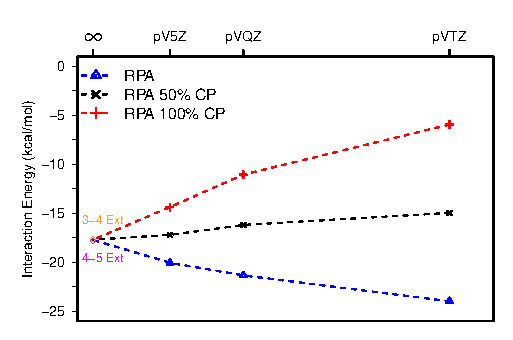
\includegraphics{extrapol.eps}
  \caption{Basis set convergence of the RPA interaction energy using a
    PBE KS reference for compound number 5 of S30L\cite{Sure15JChemTheoryComput}
    is reported. The energy expectation value of the KS determinant was computed
    using def2-QZVP\cite{Weigend03JChemPhys119p12753} 
    basis sets. $X$ denotes the cardinal number of Dunning's correlation
    consistent polarized cc-pVXZ (X=T,Q,5) basis
    sets\cite{Dunning89JChemPhys90p1007,doi:10.1063/1.464303}. All RPA
    correlation energies were computed within the frozen core
    approximation.
    %\filipp{This figure is really confusing: Does ``3-4'' mean
    %  $1/X^3 = 0$? If so, please label with $\infty$ instead and remove
    %  ``$1/X^3$'' y label. Also, please indicate the y intercept of the
    %  3-4 and 4-5 extrapolations and label them separately.}
     } \label{fig:extrapol}. 
\end{figure}

\section{S30L-CI: Charged Species with Counterions}

\begin{figure}[H]
  \centering
  \includegraphics{s30l-ci.eps}
  \caption{RPA(PBE) interaction energy errors ($\Delta E^{\text{RPA}}$)
    for S30L complexes with 
    counterions\cite{Sure15JChemTheoryComput}.}
  \label{fig:s30cirpa}
\end{figure}

\begin{figure}[H]
  \centering
  \includegraphics{mp2-ci.eps}
  \caption{MP2 interaction energy errors ($\Delta E^{\text{MP2}}$) for S30L complexes with
    counterions\cite{Sure15JChemTheoryComput}.}
  \label{fig:s30cimp2}
\end{figure}

To investigate the effect of counterions in MP2 and RPA calculations of
interaction energies of charged species, calculations were carried out for the
S30L-CI compounds, see Figures \ref{fig:s30cirpa} and \ref{fig:s30cimp2}.
The poor basis set convergence observed for complexes 29 and 30 is due to
large BSSE, which is ascribed to the fact that the sodium basis sets are
optimized for neutral atoms. Due to these basis set artifacts, counterions
were excluded from the benchmark calculations.

\section{HOMO-LUMO Gap Effect on Interaction Energies}

\begin{figure}[H]
  \centering
  \includegraphics{homo_lumo_compare.eps}
  \caption{Percentage errors of interaction energy ($\Delta E$) for
    the S66,\cite{doi:10.1021/ct2002946,doi:10.1021/ct200523a}
    L7,\cite{doi:10.1021/ct400036b} and S30L\cite{Sure15JChemTheoryComput}
    benchmark vs. the HF HOMO-LUMO gap.} 
\end{figure}

\section{ROT34 RPA Rotational Constants}

\LTcapwidth=\textwidth
\begin{spacing}{1}
\begin{longtable}{llRRR}
  \caption{Rotational constants (B$_e$) of RPA(PBE) optimized ROT34
    structures\cite{C3CP52293H,Risthaus14JComputChem35p1509} 
    using def2-TZVP\cite{Weigend05PhysChemChemPhys7p3297} and 
    def2-QZVP\cite{Weigend03JChemPhys119p12753} basis sets.} \\
    \hline
    Molecule & B$_{\text{e}}$    & \text{B}_{\text{ref}} & \text{def2-TZVP} & \text{def2-QZVP} \\
    \hline
    Ethynyl-cyclohexane & A     & 4293.9 & 4237.76 & 4290.80 \\
          & B     & 1395.9 & 1378.84 & 1394.31 \\
          & C     & 1130.2 & 1116.87 & 1129.77 \\
    isoamyl-acetate & A     & 3322.5 & 3287.81 & 3314.13 \\
          & B     & 719.8 & 719.45 & 726.51 \\
          & C     & 698   & 697.76 & 705.11 \\
    diisopropyl-ketone & A     & 3071.1 & 3031.70 & 3064.32 \\
          & B     & 1285  & 1274.55 & 1284.71 \\
          & C     & 1248.7 & 1228.17 & 1246.54 \\
    bicyclo[2.2.2]octadiene & A     & 2755.9 & 2722.34 & 2753.63 \\
          & B     & 2675.6 & 2643.22 & 2674.30 \\
          & C     & 2653.3 & 2621.95 & 2650.23 \\
    tri-ethylamine & A     & 2336.9 & 2301.45 & 2332.23 \\
    Vitamin C & A     & 1464.2 & 1441.62 & 1454.48 \\
          & B     & 768.2 & 762.09 & 770.25 \\
          & C     & 580.6 & 575.76 & 581.27 \\
    serotonine & A     & 1165.7 & 1152.57 & 1167.84 \\
          & B     & 661.2 & 654.63 & 658.47 \\
          & C     & 454   & 449.35 & 453.95 \\
    Aspirin & A     & 1166.3 & 1135.86 & 1162.10 \\
          & B     & 767.6 & 762.53 & 767.35 \\
          & C     & 513   & 504.55 & 512.23 \\
    cassyrane & A     & 862.5 & 851.03 & 860.71 \\
          & B     & 754.2 & 748.20 & 756.04 \\
          & C     & 513.7 & 508.87 & 514.36 \\
    r-(+)-limonene & A     & 3086.2 & 3046.76 & 3082.38 \\
          & B     & 723.7 & 716.83 & 724.63 \\
          & C     & 685   & 676.34 & 684.12 \\
    (-)-lupinine & A     & 1432.1 & 1413.52 & 1429.03 \\
          & B     & 820.5 & 811.04 & 821.49 \\
          & C     & 679.4 & 670.57 & 679.15 \\
    Ac-Pro-NH 2 & A     & 1523.2 & 1486.19 & 1506.76 \\
          & B     & 1070.5 & 1065.42 & 1074.41 \\
          & C     & 719.9 & 714.47 & 720.17 \\
    \hline
  \label{tab:pbe_rot34}
\end{longtable}%

\begin{longtable}{llRRR}
  \caption{Rotational constants (B$_e$) of RPA(TPSS) optimized ROT34
    structures\cite{C3CP52293H,Risthaus14JComputChem35p1509}
    using def2-TZVP\cite{Weigend05PhysChemChemPhys7p3297}
    and def2-QZVP\cite{Weigend03JChemPhys119p12753} basis sets} \\
    \hline
    Molecule & B$_{\text{e}}$  & \text{B}_{\text{ref}} & \text{def2-TZVP} & \text{def2-QZVP} \\
    \hline
    Ethynyl-cyclohexane & A     & 4293.9 & 4250.74 & 4303.30 \\
          & B     & 1395.9 & 1381.86 & 1397.40 \\
          & C     & 1130.2 & 1119.43 & 1132.40 \\
    Isoamyl-acetate & A     & 3322.5 & 3296.85 & 3323.80 \\
          & B     & 719.8 & 720.22 & 726.80 \\
          & C     & 698   & 698.66 & 705.40 \\
    Diisopropyl-ketone & A     & 3071.1 & 3039.14 & 3071.69 \\
          & B     & 1285  & 1277.08 & 1287.39 \\
          & C     & 1248.7 & 1232.32 & 1250.71 \\
    Bicyclo[2.2.2]octadiene & A     & 2755.9 & 2729.11 & 2760.40 \\
          & B     & 2675.6 & 2650.39 & 2681.40 \\
          & C     & 2653.3 & 2627.33 & 2655.60 \\
    Tri-ethylamine & A     & 2336.9 & 2307.68 & 2338.44 \\
    Vitamin C & A     & 1464.2 & 1445.25 & 1457.90 \\
          & B     & 768.2 & 762.54 & 770.80 \\
          & C     & 580.6 & 576.26 & 581.90 \\
    Serotonine & A     & 1165.7 & 1155.01 & 1170.10 \\
          & B     & 661.2 & 655.51 & 659.50 \\
          & C     & 454   & 450.10 & 454.70 \\
    Aspirin & A     & 1166.3 & 1137.69 & 1164.60 \\
          & B     & 767.6 & 763.67 & 768.30 \\
          & C     & 513   & 505.33 & 513.20 \\
    Cassyrane & A     & 862.5 & 852.89 & 862.60 \\
          & B     & 754.2 & 750.03 & 757.90 \\
          & C     & 513.7 & 510.03 & 515.60 \\
    r-(+)-Limonene & A     & 3086.2 & 3054.13 & 3089.70 \\
          & B     & 723.7 & 718.60 & 726.40 \\
          & C     & 685   & 678.05 & 685.80 \\
    (-)-Lupinine & A     & 1432.1 & 1416.16 & 1431.80 \\
          & B     & 820.5 & 812.85 & 823.30 \\
          & C     & 679.4 & 671.76 & 680.40 \\
    Ac-Pro-NH 2 & A     & 1523.2 & 1490.93 & 1511.00 \\
          & B     & 1070.5 & 1066.61 & 1075.90 \\
    & C     & 719.9 & 715.63 & 721.40 \\
    \hline
  \label{tab:tpss_rot34}
\end{longtable}

\section{L7 Total Energies}

\subsection{RPA}

\begin{longtable}[H]{lRRR}
  \caption{RPA total energies (Hartree) using a PBE KS reference
    calculated for L7 \cite{doi:10.1021/ct400036b}. The expectation value of the KS
    determinant ($\braket{\Phi_{\text{KS}}|\hat{H}|\Phi_{\text{KS}}}$)
     was computed using def2-QZVP\cite{Weigend03JChemPhys119p12753}
     basis sets, and RPA correlation energies ($E^{\text{C RPA}}$)
     were computed using Dunning's correlation-consistent basis sets
     \cite{Dunning89JChemPhys90p1007,doi:10.1063/1.464303} within the
     frozen core approximation.} \\
    \hline
    Complex & \braket{\Phi_{\text{KS}}|\hat{H}|\Phi_{\text{KS}}} &
    \text{E}^{\text{C RPA}}\text{/cc-pVTZ} & \text{E}^{\text{C
        RPA}}\text{/cc-pVQZ} \\ 
    \hline
    c2c2pd &       &       &  \\
    Supermol & -1832.10194 & -11.44473 & -12.26832 \\
    GhostA &       & -5.69823 & -6.10858 \\
    GhostB &       & -5.69823 & -6.10858 \\
    FragA & -916.06378 & -5.69242 & -6.10541 \\
    FragB & -916.06378 & -5.69242 & -6.10541 \\
    c3a   &       &       &  \\
    Supermol & -2520.54229 & -15.29536 & -16.41449 \\
    GhostA &       & -2.70719 & -2.91536 \\
    GhostB &       & -12.55437 & -13.46283 \\
    FragA & -464.60158 & -2.70259 & -2.91231 \\
    FragB & -2055.95638 & -12.54976 & -13.46041 \\
    c3gc  &       &       &  \\
    Supermol & -2988.13608 & -17.93856 & -19.26997 \\
    GhostA &       & -5.32062 & -5.74074 \\
    GhostB &       & -12.55785 & -13.46463 \\
    FragA & -932.20947 & -5.31160 & -5.73479 \\
    FragB & -2055.95623 & -12.54983 & -13.46054 \\
    cbh   &       &       &  \\
    Supermol & -1407.76620 & -10.67835 & -11.39482 \\
    GhostA &       & -5.32577 & -5.68293 \\
    GhostB &       & -5.32575 & -5.68290 \\
    FragA & -703.89120 & -5.32345 & -5.68175 \\
    FragB & -703.89123 & -5.32342 & -5.68172 \\
    gcgc  &       &       &  \\
    Supermol & -1864.45573 & -10.59006 & -11.43897 \\
    GhostA &       & -5.27724 & -5.70008 \\
    GhostB &       & -5.27723 & -5.70007 \\
    FragA & -932.23892 & -5.27170 & -5.69698 \\
    FragB & -932.23893 & -5.27169 & -5.69696 \\
    ggg   &       &       &  \\
    Supermol & -1618.42588 & -9.15944 & -9.89025 \\
    GhostA &       & -3.04366 & -3.28647 \\
    GhostB &       & -6.10143 & -6.58833 \\
    FragA & -539.49068 & -3.04155 & -3.28518 \\
    FragB & -1078.94909 & -6.09956 & -6.58716 \\
    phe   &       &       &  \\
    Supermol & -2050.50659 & -12.55229 & -13.50576 \\
    GhostA &       & -4.17245 & -4.48869 \\
    GhostB &       & -8.36625 & -9.00045 \\
    FragA & -683.49182 & -4.16886 & -4.48657 \\
    FragB & -1366.99657 & -8.36319 & -8.99862 \\
  \label{tab:pbe_l7}
\end{longtable}

\begin{longtable}[H]{lRRR}
  \caption{RPA total energies (Hartree) using a TPSS KS reference
    calculated for L7\cite{doi:10.1021/ct400036b}. The expectation value of the KS
    determinant ($\braket{\Phi_{\text{KS}}|\hat{H}|\Phi_{\text{KS}}}$)
     was computed using def2-QZVP\cite{Weigend03JChemPhys119p12753}
     basis sets, and RPA correlation energies ($E^{\text{C RPA}}$)
     were computed using Dunning's correlation-consistent basis sets
     \cite{Dunning89JChemPhys90p1007,doi:10.1063/1.464303} within the
     frozen core approximation.} \\
    \hline
    Molecule & \braket{\Phi_{\text{KS}}|\hat{H}|\Phi_{\text{KS}}} &
    E^{\text{C RPA}}\text{/cc-pVTZ} & E^{\text{C RPA}}\text{/cc-pVQZ} \\
    \hline
    c2c2pd &       &       &  \\
    Supermol & -1832.22619 & -11.21840 & -12.03318 \\
    GhostA &       & -5.58565 & -5.99157 \\
    GhostB &       & -5.58565 & -5.99157 \\
    FragA & -916.12550 & -5.57999 & -5.98843 \\
    FragB & -916.12550 & -5.57999 & -5.98843 \\
    c3a   &       &       &  \\
    Supermol & -2520.70479 & -15.00884 & -16.11625 \\
    GhostA &       & -2.65731 & -2.86297 \\
    GhostB &       & -12.31866 & -13.21797 \\
    FragA & -464.62841 & -2.65285 & -2.86002 \\
    FragB & -2056.09140 & -12.31418 & -13.21556 \\
    c3gc  &       &       &  \\
    Supermol & -2988.32515 & -17.60324 & -18.92032 \\
    GhostA &       & -5.22274 & -5.63769 \\
    GhostB &       & -12.32205 & -13.21975 \\
    FragA & -932.26226 & -5.21402 & -5.63196 \\
    FragB & -2056.09127 & -12.31424 & -13.21569 \\
    cbh   &       &       &  \\
    Supermol & -1407.89340 & -10.39751 & -11.10295 \\
    GhostA &       & -5.18644 & -5.53820 \\
    GhostB &       & -5.18642 & -5.53817 \\
    FragA & -703.95379 & -5.18421 & -5.53708 \\
    FragB & -703.95382 & -5.18418 & -5.53705 \\
    gcgc  &       &       &  \\
    Supermol & -1864.56205 & -10.39561 & -11.23408 \\
    GhostA &       & -5.18064 & -5.59834 \\
    GhostB &       & -5.18062 & -5.59832 \\
    FragA & -932.29157 & -5.17528 & -5.59534 \\
    FragB & -932.29159 & -5.17526 & -5.59532 \\
    ggg   &       &       &  \\
    Supermol & -1618.51593 & -8.99533 & -9.71722 \\
    GhostA &       & -2.98926 & -3.22914 \\
    GhostB &       & -5.99226 & -6.47325 \\
    FragA & -539.52036 & -2.98723 & -3.22790 \\
    FragB & -1079.00900 & -5.99045 & -6.47213 \\
    phe   &       &       &  \\
    Supermol & -2050.64176 & -12.28708 & -13.22815 \\
    GhostA &       & -4.08461 & -4.39679 \\
    GhostB &       & -8.18961 & -8.81560 \\
    FragA & -683.53637 & -4.08116 & -4.39475 \\
    FragB & -1367.08652 & -8.18667 & -8.81384
\end{longtable}

%\subsection{RIAXK}
%
%\begin{longtable}[H]{lRRR}
%  \caption{The beyond-RPA Perturbative corrections with the approximate
%    exchange kernal (RIAXK) total energies (Hartree) using a PBE KS reference
%    calculated for L7\cite{doi:10.1021/ct400036b}. The expectation value of the KS
%    determinant ($\braket{\Phi_{\text{KS}}|\hat{H}|\Phi_{\text{KS}}}$)
%     was computed using def2-QZVP\cite{Weigend03JChemPhys119p12753}
%     basis sets, and RPA correlation energies ($E^{\text{C RIAXK}}$)
%     were computed using Dunning's correlation-consistent basis sets
%     \cite{Dunning89JChemPhys90p1007,doi:10.1063/1.464303} within the
%     frozen core approximation.} \\
%    \hline
%    Molecule & \braket{\Phi_{\text{KS}}|\hat{H}|\Phi_{\text{KS}}}
%    & E^{\text{C RIAXK}}\text{/cc-pVTZ} & E^{\text{C RIAXK}}\text{/cc-pVQZ} \\
%    \hline
%     c2c2pd   &                &        &  \\
%     Supermol & -1832.10193  &-8.34300  & -8.84938 \\
%     GhostA   &   	     &-4.14725  & \\
%     GhostB   &   	     &-4.14725  & \\
%     FragA    &  -916.06378  &-4.14327  & -4.39702\\
%     FragB    &  -916.06378  &-4.14327  & -4.39702\\
%     c3a      &   	     &          & \\
%     Supermol & -2520.54228  &-11.20416 & -11.89417\\
%     GhostA   &   	     &-1.96895  & \\
%     GhostB   &   	     &-9.20088  & \\
%     FragA    &  -464.60158  &-1.96561  & -2.09550\\
%     FragB    & -2055.95637  &-9.19779  & -9.75836\\
%     c3gc     &   	     &          & \\
%     Supermol & -2988.13607  &-13.13384 & -13.95614\\
%     GhostA   &   	     &-3.86937  & \\
%     GhostB   &   	     &-9.20325  & \\
%     FragA    & -932.20947  &-3.86271   & -4.12535\\
%     FragB    & -2055.95623  &-9.19785  & -9.75849\\
%     cbh      &   	     &          & \\
%     Supermol & -1407.76620  &-7.46164  & -7.89597\\
%     GhostA   &   	     &-3.71651  & \\
%     GhostB   &   	     &-3.71649  & \\
%     FragA    &  -703.89119  &-3.71484  & -3.93196\\
%     FragB    &  -703.89123  &-3.71482  & -3.93193\\
%     gcgc     &   	     &-         & \\
%     Supermol & -1864.45573  &-7.70232  & -8.22940\\
%     GhostA   &   	     &-3.83307  & \\
%     GhostB   &   	     &-3.83306  & \\
%     FragA    &  -932.23892  &-3.82900  & -4.09287\\
%     FragB    &  -932.23893  &-3.82900  & -4.09286\\
%     ggg      &   	     &          & \\
%     Supermol & -1618.42588  &-6.67497  & -7.12921\\
%     GhostA   &   	     &-2.21533  & \\
%     GhostB   &   	     &-4.44524  & \\
%     FragA    &  -539.49067  &-2.21376  & -2.36506\\
%     FragB    & -1078.94909  &-4.44389  & -4.74692\\
%     phe      &   	     &          & \\
%     Supermol & -2050.50658  &-9.02738  & -9.61516\\
%     GhostA   &   	     &-2.99617  & \\
%     GhostB   &              &-6.01495  & \\
%     FragA    &  -683.49182  &-2.99353  & -3.18932\\
%     FragB    & -1366.99656  &-6.01272  & -6.40440\\
%  \label{tab:riaxk_l7}%
%\end{longtable}%
%
%\subsection{SOSEX}
%
%\begin{longtable}[H]{lRR}
%  \caption{The beyond-RPA Perturbative corrections with the bare
%    second-order screened exchange (SOSEX) total energies (Hartree)
%    using a PBE KS reference calculated for L7 \cite{doi:10.1021/ct400036b}. The
%    expectation value of the KS determinant ($\braket{\Phi_{\text{KS}}|\hat{H}|\Phi_{\text{KS}}}$)
%     was computed using def2-QZVP\cite{Weigend03JChemPhys119p12753}
%     basis sets, and RPA correlation energies ($E^{\text{C SOSEX}}$)
%     were computed using Dunning's correlation-consistent basis sets
%     \cite{Dunning89JChemPhys90p1007,doi:10.1063/1.464303} within the
%     frozen core approximation.} \\
%    \hline
%    Molecule & \braket{\Phi_{\text{KS}}|\hat{H}|\Phi_{\text{KS}}} & E^{\text{C SOSEX}}\text{/cc-pVTZ} \\
%    \hline
%     c2c2pd   &               &            \\
%     Supermol &-1832.10193   &   -7.53048 \\
%     GhostA   &	             &   -3.74121 \\
%     GhostB   &	             &   -3.74121 \\
%     FragA    &-916.06378   &    -3.73755 \\
%     FragB    &-916.06378   &    -3.73755 \\
%     c3a      &              &             \\
%     Supermol &-2520.54228   &   -10.11924 \\
%     GhostA   &	             &    -1.76908 \\
%     GhostB   &	             &    -8.31592 \\
%     FragA    &-464.60158   &     -1.76605 \\
%     FragB    &-2055.95637   &    -8.31312 \\
%     c3gc     &	             &             \\
%     Supermol &-2988.13607   &   -11.85645 \\
%     GhostA   &	             &    -3.47717 \\
%     GhostB   &	             &    -8.31805 \\
%     FragA    &-932.20947   &     -3.47106 \\
%     FragB    &-2055.95623   &    -8.31313 \\
%     cbh      &	             &             \\
%     Supermol &-1407.76620   &    -6.66955 \\
%     GhostA   &	             &    -3.32055 \\
%     GhostB   &	             &    -3.32052 \\
%     FragA    &-703.89120   &     -3.31898 \\
%     FragB    &-703.89123   &     -3.31896 \\
%     gcgc     &	             &             \\
%     Supermol &-1864.45573   &    -6.93559 \\
%     GhostA   &	             &    -3.45005 \\
%     GhostB   &	             &    -3.45004 \\
%     FragA    &-932.23892   &     -3.44635 \\
%     FragB    &-932.23893   &     -3.44634 \\
%     ggg      &	             &             \\
%     Supermol &-1618.42588   &    -6.00181 \\
%     GhostA   &	             &    -1.99104 \\
%     GhostB   &	             &    -3.99696 \\
%     FragA    & -539.49068   &    -1.98964 \\
%     FragB    &-1078.94909   &    -3.99573 \\
%     phe      &	             &             \\
%     Supermol &-2050.50658   &    -8.09874 \\
%     GhostA   &	             &    -2.68571 \\
%     GhostB   &	             &    -5.39489 \\
%     FragA    &-683.49182   &     -2.68329 \\
%     FragB    &-1366.99656   &    -5.39286 \\
%  \label{tab:sosex_l7}%
%\end{longtable}%

\subsection{MP2}

\begin{longtable}[H]{lRRRRR}
  \caption{MP2 total energies (Hartree) calculated for L7.\cite{doi:10.1021/ct400036b}
    The expectation value of the HF determinant ($\braket{\Phi_{\text{HF}}|\hat{H}|\Phi_{\text{HF}}}$)
     was computed using def2-QZVP\cite{Weigend03JChemPhys119p12753}
     basis sets. MP2 opposite spin (OS) and same spin (SS) contributions
     were computed using Dunning's correlation-consistent basis sets
     \cite{Dunning89JChemPhys90p1007,doi:10.1063/1.464303} within the
     frozen core approximation.}\\
  \hline
  Molecule & \braket{\Phi_{\text{HF}}|\hat{H}|\Phi_{\text{HF}}} &
  \text{OS/cc-pVTZ} & \text{SS/cc-pVTZ} &
  \text{OS/cc-pVQZ} & \text{SS/cc-pVQZ} \\
  \hline
    c2c2pd   &                      &               &               &               &               \\
    Supermol & -1832.53892          & -5.47067      & -2.04730      & -5.86410      & -2.10916      \\
    GhostA   &                      & -2.71467      & -1.00418      & -2.91031      & -1.03422      \\
    GhostB   &                      & -2.71467      & -1.00418      & -2.91031      & -1.03422      \\
    FragA    & -916.28200           & -2.71176      & -1.00325      & -2.90883      & -1.03386      \\
    FragB    & -916.28200           & -2.71176      & -1.00325      & -2.90883      & -1.03386      \\
    c3a      &                      &               &               &               &               \\
    Supermol & -2521.14726          & -7.34454      & -2.80686      & -7.88010      & -2.89259      \\
    GhostA   &                      & -1.30037      & -0.47317      & -1.40016      & -0.48936      \\
    GhostB   &                      & -6.01712      & -2.30736      & -6.45122      & -2.37556      \\
    FragA    & -464.71264           & -1.29805      & -0.47232      & -1.39874      & -0.48893      \\
    FragB    & -2056.44903          & -6.01483      & -2.30672      & -6.45010      & -2.37534      \\
    c3gc     &                      &               &               &               &               \\
    Supermol & -2988.86611          & -8.61615      & -3.27733      & -9.25385      & -3.38076      \\
    GhostA   &                      & -2.55097      & -0.92429      & -2.75238      & -0.95727      \\
    GhostB   &                      & -6.01883      & -2.30783      & -6.45203      & -2.37572      \\
    FragA    & -932.44427           & -2.54637      & -0.92248      & -2.74963      & -0.95638      \\
    FragB    & -2056.44899          & -6.01483      & -2.30668      & -6.45013      & -2.37533      \\
    cbh      &                      &               &               &               &               \\
    Supermol & -1408.13226          & -4.92635      & -1.42224      & -5.26374      & -1.46878      \\
    GhostA   &                      & -2.45614      & -0.70421      & -2.62435      & -0.72714      \\
    GhostB   &                      & -2.45613      & -0.70420      & -2.62435      & -0.72713      \\
    FragA    & -704.07190           & -2.45522      & -0.70398      & -2.62389      & -0.72706      \\
    FragB    & -704.07192           & -2.45522      & -0.70397      & -2.62388      & -0.72705      \\
    gcgc     &                      &               &               &               &               \\
    Supermol & -1864.91452          & -5.08296      & -1.85232      & -5.49055      & -1.92074      \\
    GhostA   &                      & -2.53018      & -0.91549      & -2.73300      & -0.94890      \\
    GhostB   &                      & -2.53018      & -0.91549      & -2.73300      & -0.94890      \\
    FragA    & -932.46677           & -2.52736      & -0.91442      & -2.73155      & -0.94842      \\
    FragB    & -932.46677           & -2.52736      & -0.91442      & -2.73155      & -0.94842      \\
    ggg      &                      &               &               &               &               \\
    Supermol & -1618.81849          & -4.41740      & -1.62090      & -4.76851      & -1.68023      \\
    GhostA   &                      & -1.46580      & -0.53418      & -1.58237      & -0.55357      \\
    GhostB   &                      & -2.94184      & -1.07833      & -3.17574      & -1.11770      \\
    FragA    & -539.62086           & -1.46471      & -0.53375      & -1.58177      & -0.55336      \\
    FragB    & -1079.21034          & -2.94091      & -1.07800      & -3.17520      & -1.11753      \\
    phe      &                      &               &               &               &               \\
    Supermol & -2051.01827          & -5.95610      & -2.04333      & -6.41179      & -2.11563      \\
    GhostA   &                      & -1.98010      & -0.67389      & -2.13118      & -0.69749      \\
    GhostB   &                      & -3.96969      & -1.35934      & -4.27276      & -1.40714      \\
    FragA    & -683.65933           & -1.97838      & -0.67322      & -2.13024      & -0.69722      \\
    FragB    & -1367.33696          & -3.96821      & -1.35878      & -4.27194      & -1.40691     
\end{longtable}

\section{S30L Total Energies}

\subsection{RPA}

\begin{longtable}{lRRR}
  \caption{RPA total energies (Hartree) using a PBE KS reference
    calculated for S30L\cite{Sure15JChemTheoryComput}. The expectation value of the KS
    determinant ($\braket{\Phi_{\text{KS}}|\hat{H}|\Phi_{\text{KS}}}$)
    was computed using def2-QZVP\cite{Weigend03JChemPhys119p12753}
    basis sets, and RPA correlation energies ($E^{\text{C RPA}}$)
    were computed using Dunning's correlation-consistent basis sets
    \cite{Dunning89JChemPhys90p1007,doi:10.1063/1.464303} within the
    frozen core approximation.} \\
  \hline
  Molecule & \braket{\Phi_{\text{KS}}|\hat{H}|\Phi_{\text{KS}}} &
  E^{\text{C RPA}}\text{/cc-pVTZ} & E^{\text{C RPA}}\text{/cc-pVQZ} \\
  \hline
    \multicolumn{1}{l}{1} &       &       & \\ 
    Supermol & -2282.6035 & -14.3861 & -15.4115 \\
    MonomerA &       & -10.3682 & -11.1023 \\
    MonomerB &       & -3.9414 & -4.2351 \\
    GhostA &       & -10.3777 & -11.1071 \\
    GhostB &       & -3.9492 & -4.2396 \\
    FragA & -1608.0899 & -10.3679 & -11.102 \\
    FragB & -674.5397 & -3.9421 & -4.2357 \\
    \multicolumn{1}{l}{2} &       &       &  \\
    Supermol & -2022.2942 & -12.8822 & -13.7977 \\
    MonomerA &       & -10.3674 & -11.1016 \\
    MonomerB &       & -2.4581 & -2.6412 \\
    GhostA &       & -10.3748 & -11.1054 \\
    GhostB &       & -2.4631 & -2.6442 \\
    FragA & -1608.0899 & -10.3679 & -11.102 \\
    FragB & -414.2268 & -2.4589 & -2.6419 \\
    \multicolumn{1}{l}{3} &       &       &  \\
    Supermol & -3804.9443 & -22.0993 & -23.8082 \\
    MonomerA &       & -15.5758 & -16.7703 \\
    MonomerB &       & -6.4041 & -6.9233 \\
    GhostA &       & -15.5896 & -16.7782 \\
    GhostB &       & -6.419 & -6.9318 \\
    FragA & -2622.5691 & -15.6156 & -16.8085 \\
    FragB & -1182.4172 & -6.4046 & -6.9236 \\
    \multicolumn{1}{l}{4} &       &       &  \\
    Supermol & -3698.2182 & -19.3261 & -20.8244 \\
    MonomerA &       & -15.5782 & -16.7726 \\
    MonomerB &       & -3.6739 & -3.9799 \\
    GhostA &       & -15.5864 & -16.7773 \\
    GhostB &       & -3.6845 & -3.9862 \\
    FragA & -2622.5691 & -15.6156 & -16.8085 \\
    FragB & -1075.6528 & -3.6732 & -3.9792 \\
    \multicolumn{1}{l}{5} &       &       &  \\
    Supermol & -3006.0751 & -17.8185 & -19.1584 \\
    MonomerA &       & -11.3139 & -12.1376 \\
    MonomerB &       & -6.4063 & -6.9254 \\
    GhostA &       & -11.3247 & -12.1434 \\
    GhostB &       & -6.4183 & -6.9323 \\
    FragA & -1823.6917 & -11.3265 & -12.15 \\
    FragB & -1182.4156 & -6.4047 & -6.9237 \\
    \multicolumn{1}{l}{6} &       &       &  \\
    Supermol & -2498.1857 & -15.3516 & -16.4665 \\
    MonomerA &       & -11.3167 & -12.1404 \\
    MonomerB &       & -3.9431 & -4.2368 \\
    GhostA &       & -11.3273 & -12.1461 \\
    GhostB &       & -3.9526 & -4.242 \\
    FragA & -1823.6917 & -11.3265 & -12.15 \\
    FragB & -674.539 & -3.9421 & -4.2357 \\
    \multicolumn{1}{l}{7} &       &       &  \\
    Supermol & -3968.2604 & -24.8319 & -26.6149 \\
    MonomerA &       & -15.1913 & -16.2903 \\
    MonomerB &       & -9.5103 & -10.198 \\
    GhostA &       & -15.2046 & -16.2972 \\
    GhostB &       & -9.5215 & -10.2042 \\
    FragA & -2442.0869 & -15.1913 & -16.2904 \\
    FragB & -1526.2397 & -9.5119 & -10.1993 \\
    \multicolumn{1}{l}{8} &       &       &  \\
    Supermol & -4578.8194 & -28.6314 & -30.6885 \\
    MonomerA &       & -17.0864 & -18.3227 \\
    MonomerB &       & -11.4007 & -12.2257 \\
    GhostA &       & -17.101 & -18.3303 \\
    GhostB &       & -11.4131 & -12.2326 \\
    FragA & -2747.3624 & -17.0867 & -18.3229 \\
    FragB & -1831.5284 & -11.4026 & -12.2273 \\
    \multicolumn{1}{l}{9} &       &       &  \\
    Supermol & -4560.6742 & -27.845 & -29.8549 \\
    MonomerA &       & -14.2456 & -15.2733 \\
    MonomerB &       & -13.4731 & -14.4631 \\
    GhostA &       & -14.2619 & -15.2813 \\
    GhostB &       & -13.4849 & -14.4703 \\
    FragA & -2288.7357 & -14.2451 & -15.2728 \\
    FragB & -2271.9966 & -13.4731 & -14.4631 \\
    \multicolumn{1}{l}{10} &       &       &  \\
    Supermol & -4939.4274 & -30.1014 & -32.2742 \\
    MonomerA &       & -14.2465 & -15.2742 \\
    MonomerB &       & -15.72 & -16.8738 \\
    GhostA &       & -14.2635 & -15.2826 \\
    GhostB &       & -15.7331 & -16.8815 \\
    FragA & -2288.7357 & -14.2451 & -15.2728 \\
    FragB & -2650.7568 & -15.7201 & -16.8739 \\
    \multicolumn{1}{l}{11} &       &       &  \\
    Supermol & -8152.4322 & -28.3007 & -30.4264 \\
    MonomerA &       & -14.6641 & -15.81 \\
    MonomerB &       & -13.4737 & -14.4637 \\
    GhostA &       & -14.6869 & -15.8223 \\
    GhostB &       & -13.4881 & -14.4721 \\
    FragA & -5880.5281 & -14.656 & -15.8021 \\
    FragB & -2271.9933 & -13.4731 & -14.4631 \\
    \multicolumn{1}{l}{12} &       &       &  \\
    Supermol & -8531.1932 & -30.5476 & -32.8368 \\
    MonomerA &       & -14.6639 & -15.8098 \\
    MonomerB &       & -15.7203 & -16.8741 \\
    GhostA &       & -14.6869 & -15.8221 \\
    GhostB &       & -15.7348 & -16.8825 \\
    FragA & -5880.5281 & -14.656 & -15.8021 \\
    FragB & -2650.753 & -15.7201 & -16.8739 \\
    \multicolumn{1}{l}{13} &       &       &  \\
    Supermol & -5108.5081 & -31.2943 & -33.6219 \\
    MonomerA &       & -29.4022 & -31.5949 \\
    MonomerB &       & -1.8273 & -1.9648 \\
    GhostA &       & -29.4125 & -31.6008 \\
    GhostB &       & -1.8329 & -1.968 \\
    FragA & -4822.4714 & -29.4025 & -31.5951 \\
    FragB & -286.0548 & -1.8275 & -1.965 \\
    \multicolumn{1}{l}{14} &       &       &  \\
    Supermol & -5451.003 & -31.2617 & -33.5927 \\
    MonomerA &       & -29.4023 & -31.5949 \\
    MonomerB &       & -1.7845 & -1.9255 \\
    GhostA &       & -29.413 & -31.601 \\
    GhostB &       & -1.7915 & -1.9295 \\
    FragA & -4822.4714 & -29.4025 & -31.5951 \\
    FragB & -628.557 & -1.7852 & -1.926 \\
    \DIFdelbegin %DIFDELCMD < \multicolumn{1}{l}{15} %%%
\DIFdelend \DIFaddbegin \multicolumn{1}{l}{15\textsuperscript{\emph{a}}} \DIFaddend &       &       &  \\
    Supermol & -3675.2176 & -14.7326 & -16.2915 \\
    MonomerA &       & -11.9254 & -13.2872 \\
    MonomerB &       & -2.7639 & -2.9561 \\
    GhostA &       & -11.9343 & -13.2967 \\
    GhostB &       & -2.7639 & -2.9575 \\
    FragA & -3290.7594 & -11.9046 & -13.2837 \\
    FragB & -384.4778 & -2.7635 & -2.9558 \\
    \DIFdelbegin %DIFDELCMD < \multicolumn{1}{l}{16} %%%
\DIFdelend \DIFaddbegin \multicolumn{1}{l}{16\textsuperscript{\emph{a}}} \DIFaddend &       &       &  \\
    Supermol & -3843.8773 & -15.7507 & -17.3854 \\
    MonomerA &       & -11.929 & -13.2915 \\
    MonomerB &       & -3.7657 & -4.0321 \\
    GhostA &       & -11.9415 & -13.3046 \\
    GhostB &       & -3.769 & -4.0338 \\
    FragA & -3290.7594 & -11.9046 & -13.2837 \\
    FragB & -553.1469 & -3.7632 & -4.0297 \\
    \multicolumn{1}{l}{17} &       &       &  \\
    Supermol & -3272.8435 & -20.563 & -22.0772 \\
    MonomerA &       & -18.1627 & -19.4879 \\
    MonomerB &       & -2.3431 & -2.5332 \\
    GhostA &       & -18.1705 & -19.492 \\
    GhostB &       & -2.352 & -2.5384 \\
    FragA & -2859.1414 & -18.1665 & -19.4917 \\
    FragB & -413.6998 & -2.3417 & -2.5316 \\
    \multicolumn{1}{l}{18} &       &       &  \\
    Supermol & -3238.4198 & -20.3635 & -21.8577 \\
    MonomerA &       & -18.1623 & -19.4875 \\
    MonomerB &       & -2.1467 & -2.3162 \\
    GhostA &       & -18.1686 & -19.4909 \\
    GhostB &       & -2.154 & -2.3206 \\
    FragA & -2859.1414 & -18.1665 & -19.4917 \\
    FragB & -379.2953 & -2.1448 & -2.3142 \\
    \multicolumn{1}{l}{19} &       &       &  \\
    Supermol & -4522.1939 & -25.7142 & -27.8068 \\
    MonomerA &       & -23.8758 & -25.8382 \\
    MonomerB &       & -1.7969 & -1.9291 \\
    GhostA &       & -23.8835 & -25.8426 \\
    GhostB &       & -1.8012 & -1.9315 \\
    FragA & -4252.1351 & -23.874 & -25.8364 \\
    FragB & -270.0728 & -1.7973 & -1.9295 \\
    \multicolumn{1}{l}{20} &       &       &  \\
    Supermol & -4639.2815 & -26.6214 & -28.772 \\
    MonomerA &       & -23.876 & -25.8383 \\
    MonomerB &       & -2.6842 & -2.8753 \\
    GhostA &       & -23.8868 & -25.8446 \\
    GhostB &       & -2.6897 & -2.8783 \\
    FragA & -4252.1351 & -23.874 & -25.8364 \\
    FragB & -387.174 & -2.6848 & -2.8758 \\
    \multicolumn{1}{l}{21} &       &       &  \\
    Supermol & -4651.5444 & -26.8731 & -28.9764 \\
    MonomerA &       & -23.6662 & -25.5499 \\
    MonomerB &       & -3.1325 & -3.3558 \\
    GhostA &       & -23.6793 & -25.5576 \\
    GhostB &       & -3.138 & -3.3589 \\
    FragA & -4188.6034 & -23.6676 & -25.5511 \\
    FragB & -462.9564 & -3.1333 & -3.3565 \\
    \multicolumn{1}{l}{22} &       &       &  \\
    Supermol & -2888.8396 & -18.0939 & -19.4487 \\
    MonomerA &       & -7.817 & -8.3914 \\
    MonomerB &       & -10.2398 & -11.0197 \\
    GhostA &       & -7.8214 & -8.3939 \\
    GhostB &       & -10.2466 & -11.0238 \\
    FragA & -1219.5393 & -7.8113 & -8.3859 \\
    FragB & -1669.2876 & -10.2373 & -11.0172 \\
    \multicolumn{1}{l}{23} &       &       &  \\
    Supermol & -2327.7731 & -14.5653 & -15.6303 \\
    MonomerA &       & -8.7772 & -9.4075 \\
    MonomerB &       & -5.761 & -6.1951 \\
    GhostA &       & -8.7828 & -9.4107 \\
    GhostB &       & -5.7629 & -6.1964 \\
    FragA & -1370.3733 & -8.7754 & -9.4056 \\
    FragB & -957.3327 & -5.7563 & -6.1906 \\
    \multicolumn{1}{l}{24} &       &       &  \\
    Supermol & -5075.5677 & -30.0687 & -32.3714 \\
    MonomerA &       & -23.6717 & -25.5549 \\
    MonomerB &       & -6.2815 & -6.7065 \\
    GhostA &       & -23.6987 & -25.5703 \\
    GhostB &       & -6.2896 & -6.7108 \\
    FragA & -4188.6033 & -23.6676 & -25.5511 \\
    FragB & -886.8502 & -6.2823 & -6.7069 \\
    \multicolumn{1}{l}{25} &       &       &  \\
    Supermol & -3205.8668 & -20.375 & -21.8285 \\
    MonomerA &       & -15.9204 & -17.061 \\
    MonomerB &       & -4.3762 & -4.6909 \\
    GhostA &       & -15.9277 & -17.0654 \\
    GhostB &       & -4.3836 & -4.6951 \\
    FragA & -2517.1538 & -15.9191 & -17.0594 \\
    FragB & -688.744 & -4.3758 & -4.6905 \\
    \multicolumn{1}{l}{26} &       &       &  \\
    Supermol & -3205.8714 & -20.3744 & -21.8279 \\
    MonomerA &       & -15.9206 & -17.0612 \\
    MonomerB &       & -4.3756 & -4.6902 \\
    GhostA &       & -15.9279 & -17.0655 \\
    GhostB &       & -4.3829 & -4.6944 \\
    FragA & -2517.1538 & -15.9191 & -17.0594 \\
    FragB & -688.7489 & -4.3752 & -4.6899 \\
    \multicolumn{1}{l}{27} &       &       &  \\
    Supermol & -3803.0579 & -21.8872 & -23.6068 \\
    MonomerA &       & -20.2933 & -21.9071 \\
    MonomerB &       & -1.5519 & -1.6584 \\
    GhostA &       & -20.304 & -21.9132 \\
    GhostB &       & -1.5546 & -1.6599 \\
    FragA & -3590.2294 & -20.2923 & -21.9063 \\
    FragB & -212.7372 & -1.552 & -1.6585 \\
    \multicolumn{1}{l}{28} &       &       &  \\
    Supermol & -3764.0188 & -21.5865 & -23.2867 \\
    MonomerA &       & -20.2944 & -21.908 \\
    MonomerB &       & -1.2597 & -1.3466 \\
    GhostA &       & -20.3031 & -21.9131 \\
    GhostB &       & -1.2618 & -1.3477 \\
    FragA & -3590.2294 & -20.2923 & -21.9063 \\
    FragB & -173.6958 & -1.2598 & -1.3466 \\
    \multicolumn{1}{l}{29} &       &       &  \\
    Supermol & -2629.559 & -16.7232 & -17.9518 \\
    MonomerA &       & -15.4126 & -16.5345 \\
    MonomerB &       & -1.256 & -1.3658 \\
    GhostA &       & -15.4178 & -16.5374 \\
    GhostB &       & -1.2718 & -1.3753 \\
    FragA & -2402.2278 & -15.4152 & -16.5371 \\
    FragB & -227.2886 & -1.2563 & -1.3658 \\
    \multicolumn{1}{l}{30} &       &       &  \\
    Supermol & -2820.0934 & -17.8965 & -19.2102 \\
    MonomerA &       & -15.4093 & -16.5312 \\
    MonomerB &       & -2.4265 & -2.6206 \\
    GhostA &       & -15.4153 & -16.5345 \\
    GhostB &       & -2.4406 & -2.629 \\
    FragA & -2402.2278 & -15.4152 & -16.5371 \\
    FragB & -417.8351 & -2.4258 & -2.6198 \\
    23-ci &       &       &  \\
    Supermol & -2787.4024 & -14.9403 & -16.0463 \\
    MonomerA &       & -8.7768 & -9.4071 \\
    MonomerB &       & -6.0929 & -6.5724 \\
    GhostA &       & -8.7833 & -9.411 \\
    GhostB &       & -6.0981 & -6.5756 \\
    FragA & -1370.3715 & -8.7771 & -9.4073 \\
    FragB & -1416.9879 & -6.0941 & -6.5722 \\
    24-ci &       &       &  \\
    Supermol & -5994.888 & -30.7526 & -33.146 \\
    MonomerA &       & -23.6759 & -25.5593 \\
    MonomerB &       & -6.956 & -7.4718 \\
    GhostA &       & -23.7023 & -25.5744 \\
    GhostB &       & -6.9643 & -7.4765 \\
    FragA & -4188.6033 & -23.6676 & -25.5511 \\
    FragB & -1806.2926 & -6.9579 & -7.4735 \\
    25-ci &       &       &  \\
    Supermol & -5044.808 & -21.8282 & -23.4514 \\
    MonomerA &       & -17.3695 & -18.679 \\
    MonomerB &       & -4.3761 & -4.6908 \\
    GhostA &       & -17.3788 & -18.6846 \\
    GhostB &       & -4.385 & -4.6957 \\
    FragA & -4356.1013 & -17.3626 & -18.6726 \\
    FragB & -688.7431 & -4.3768 & -4.6914 \\
    26-ci &       &       &  \\
    Supermol & -5044.812 & -21.8281 & -23.4513 \\
    MonomerA &       & -17.3699 & -18.6794 \\
    MonomerB &       & -4.3756 & -4.6902 \\
    GhostA &       & -17.3792 & -18.6847 \\
    GhostB &       & -4.3843 & -4.695 \\
    FragA & -4356.1013 & -17.3626 & -18.6726 \\
    FragB & -688.748 & -4.3763 & -4.6909 \\
    27-ci &       &       &  \\
    Supermol & -4262.6861 & -22.2332 & -23.9975 \\
    MonomerA &       & -20.2966 & -21.9104 \\
    MonomerB &       & -1.8886 & -2.04 \\
    GhostA &       & -20.307 & -21.9165 \\
    GhostB &       & -1.8918 & -2.042 \\
    FragA & -3590.2075 & -20.2973 & -21.911 \\
    FragB & -672.4669 & -1.8893 & -2.0406 \\
    28-ci &       &       &  \\
    Supermol & -4223.6435 & -21.9351 & -23.68 \\
    MonomerA &       & -20.2979 & -21.9116 \\
    MonomerB &       & -1.5966 & -1.7284 \\
    GhostA &       & -20.3066 & -21.9167 \\
    GhostB &       & -1.5994 & -1.7301 \\
    FragA & -3590.2075 & -20.2973 & -21.911 \\
    FragB & -633.4264 & -1.5971 & -1.7288 \\
    29-ci &       &       &  \\
    Supermol & -2791.4094 & -16.7624 & -18.0883 \\
    MonomerA &       & -15.4134 & -16.5353 \\
    MonomerB &       & -1.284 & -1.3951 \\
    GhostA &       & -15.423 & -16.5401 \\
    GhostB &       & -1.3082 & -1.511 \\
    FragA & -2402.2265 & -15.4159 & -16.5377 \\
    FragB & -389.1573 & -1.283 & -1.3937 \\
    30-ci &       &       &  \\
    Supermol & -2981.9388 & -17.9415 & -19.3564 \\
    MonomerA &       & -15.413 & -16.5347 \\
    MonomerB &       & -2.4517 & -2.6488 \\
    GhostA &       & -15.4249 & -16.5407 \\
    GhostB &       & -2.4763 & -2.7688 \\
    FragA & -2402.2265 & -15.4159 & -16.5377 \\
    FragB & -579.6974 & -2.4493 & -2.6471 \\
  \hline
\end{longtable}
\DIFaddbegin \vspace{-0.3cm}
\DIFadd{\textsuperscript{\emph{a}} Halogen atoms used correlation consistent
small core relativistic pseudopotentials.\mbox{%DIFAUXCMD
\cite{doi:10.1063/1.1622924,doi:10.1021/jp065887l}
}\hspace{0pt}%DIFAUXCMD
}\DIFaddend 

\begin{longtable}{lRRR}
  \caption{RPA total energies (Hartree) using a TPSS KS reference
    calculated for S30L\cite{Sure15JChemTheoryComput}. The expectation value of the KS
    determinant ($\braket{\Phi_{\text{KS}}|\hat{H}|\Phi_{\text{KS}}}$)
    was computed using def2-QZVP\cite{Weigend03JChemPhys119p12753}
    basis sets, and RPA correlation energies ($E^{\text{C RPA}}$)
    were computed using Dunning's correlation-consistent basis sets
    \cite{Dunning89JChemPhys90p1007,doi:10.1063/1.464303} within the
    frozen core approximation.} \\
  \hline
  Molecule & \braket{\Phi_{\text{KS}}|\hat{H}|\Phi_{\text{KS}}} &
  E^{\text{C RPA}}\text{/cc-pVTZ} & E^{\text{C RPA}}\text{/cc-pVQZ} \\
  \hline
    \multicolumn{1}{l}{1} &       &       &  \\
    Supermol & -2282.7577 & -14.0966 & -15.1104 \\
    MonomerA &       & -10.1548 & -10.8809 \\
    MonomerB &       & -3.8679 & -4.1579 \\
    GhostA &       & -10.164 & -10.8856 \\
    GhostB &       & -3.8755 & -4.1622 \\
    FragA & -1608.202 & -10.1544 & -10.8806 \\
    FragB & -674.5798 & -3.8685 & -4.1584 \\
    \multicolumn{1}{l}{2} &       &       &  \\
    Supermol & -2022.4327 & -12.6193 & -13.5246 \\
    MonomerA &       & -10.154 & -10.8802 \\
    MonomerB &       & -2.4103 & -2.5911 \\
    GhostA &       & -10.1612 & -10.8839 \\
    GhostB &       & -2.4152 & -2.594 \\
    FragA & -1608.202 & -10.1544 & -10.8806 \\
    FragB & -414.2519 & -2.411 & -2.5917 \\
    \multicolumn{1}{l}{3} &       &       &  \\
    Supermol & -3805.1744 & -21.6698 & -23.3581 \\
    MonomerA &       & -15.2622 & -16.4422 \\
    MonomerB &       & -6.2922 & -6.8051 \\
    GhostA &       & -15.2756 & -16.4499 \\
    GhostB &       & -6.3066 & -6.8134 \\
    FragA & -2622.7338 & -15.3007 & -16.4791 \\
    FragB & -1182.4802 & -6.2926 & -6.8053 \\
    \multicolumn{1}{l}{4} &       &       &  \\
    Supermol & -3698.4198 & -18.9469 & -20.4269 \\
    MonomerA &       & -15.2646 & -16.4444 \\
    MonomerB &       & -3.6112 & -3.9133 \\
    GhostA &       & -15.2726 & -16.449 \\
    GhostB &       & -3.6214 & -3.9195 \\
    FragA & -2622.7338 & -15.3007 & -16.4791 \\
    FragB & -1075.6883 & -3.6105 & -3.9126 \\
    \multicolumn{1}{l}{5} &       &       &  \\
    Supermol & -3006.2649 & -17.4748 & -18.7989 \\
    MonomerA &       & -11.0855 & -11.8994 \\
    MonomerB &       & -6.2942 & -6.8069 \\
    GhostA &       & -11.0959 & -11.9052 \\
    GhostB &       & -6.3059 & -6.8138 \\
    FragA & -1823.8147 & -11.0976 & -11.9114 \\
    FragB & -1182.4801 & -6.2927 & -6.8053 \\
    \multicolumn{1}{l}{6} &       &       &  \\
    Supermol & -2498.3511 & -15.047 & -16.1487 \\
    MonomerA &       & -11.0882 & -11.9022 \\
    MonomerB &       & -3.8696 & -4.1596 \\
    GhostA &       & -11.0984 & -11.9078 \\
    GhostB &       & -3.8788 & -4.1647 \\
    FragA & -1823.8147 & -11.0976 & -11.9114 \\
    FragB & -674.5798 & -3.8685 & -4.1584 \\
    \multicolumn{1}{l}{7} &       &       &  \\
    Supermol & -3968.5285 & -24.3333 & -26.0948 \\
    MonomerA &       & -14.8866 & -15.9722 \\
    MonomerB &       & -9.32 & -9.9993 \\
    GhostA &       & -14.8994 & -15.9789 \\
    GhostB &       & -9.331 & -10.0054 \\
    FragA & -2442.2507 & -14.8866 & -15.9722 \\
    FragB & -1526.342 & -9.3215 & -10.0006 \\
    \multicolumn{1}{l}{8} &       &       &  \\
    Supermol & -4579.1286 & -28.0562 & -30.0886 \\
    MonomerA &       & -16.7436 & -17.9647 \\
    MonomerB &       & -11.1724 & -11.9873 \\
    GhostA &       & -16.7577 & -17.9722 \\
    GhostB &       & -11.1845 & -11.994 \\
    FragA & -2747.5468 & -16.7438 & -17.9649 \\
    FragB & -1831.6512 & -11.1741 & -11.9887 \\
    \multicolumn{1}{l}{9} &       &       &  \\
    Supermol & -4560.9642 & -27.3461 & -29.3378 \\
    MonomerA &       & -13.9668 & -14.9835 \\
    MonomerB &       & -13.2556 & -14.2378 \\
    GhostA &       & -13.9827 & -14.9914 \\
    GhostB &       & -13.2671 & -14.2449 \\
    FragA & -2288.8868 & -13.9664 & -14.9831 \\
    FragB & -2272.1332 & -13.2556 & -14.2378 \\
    \multicolumn{1}{l}{10} &       &       &  \\
    Supermol & -4939.7405 & -29.5655 & -31.719 \\
    MonomerA &       & -13.9677 & -14.9844 \\
    MonomerB &       & -15.4659 & -16.6107 \\
    GhostA &       & -13.9842 & -14.9927 \\
    GhostB &       & -15.4787 & -16.6183 \\
    FragA & -2288.8868 & -13.9664 & -14.9831 \\
    FragB & -2650.9162 & -15.466 & -16.6107 \\
    \multicolumn{1}{l}{11} &       &       &  \\
    Supermol & -8152.7465 & -27.7993 & -29.9051 \\
    MonomerA &       & -14.3842 & -15.5172 \\
    MonomerB &       & -13.2561 & -14.2383 \\
    GhostA &       & -14.4063 & -15.5292 \\
    GhostB &       & -13.2703 & -14.2467 \\
    FragA & -5880.6996 & -14.3763 & -15.5094 \\
    FragB & -2272.1332 & -13.2556 & -14.2378 \\
    \multicolumn{1}{l}{12} &       &       &  \\
    Supermol & -8531.5304 & -30.0099 & -32.2779 \\
    MonomerA &       & -14.3839 & -15.5169 \\
    MonomerB &       & -15.4662 & -16.611 \\
    GhostA &       & -14.4063 & -15.5291 \\
    GhostB &       & -15.4804 & -16.6193 \\
    FragA & -5880.6996 & -14.3763 & -15.5094 \\
    FragB & -2650.9162 & -15.466 & -16.6107 \\
    \multicolumn{1}{l}{13} &       &       &  \\
    Supermol & -5108.8535 & -30.644 & -32.9427 \\
    MonomerA &       & -28.7981 & -30.9638 \\
    MonomerB &       & -1.7844 & -1.9199 \\
    GhostA &       & -28.808 & -30.9696 \\
    GhostB &       & -1.7898 & -1.923 \\
    FragA & -4822.7941 & -28.7983 & -30.9639 \\
    FragB & -286.0757 & -1.7846 & -1.9201 \\
    \multicolumn{1}{l}{14} &       &       &  \\
    Supermol & -5451.3495 & -30.6123 & -32.9145 \\
    MonomerA &       & -28.7982 & -30.9638 \\
    MonomerB &       & -1.7427 & -1.8816 \\
    GhostA &       & -28.8085 & -30.9698 \\
    GhostB &       & -1.7494 & -1.8855 \\
    FragA & -4822.7941 & -28.7983 & -30.9639 \\
    FragB & -628.5787 & -1.7433 & -1.8821 \\
    \DIFdelbegin %DIFDELCMD < \multicolumn{1}{l}{15} %%%
\DIFdelend \DIFaddbegin \multicolumn{1}{l}{15\textsuperscript{\emph{a}}} \DIFaddend &       &       &  \\
    Supermol & -3675.3661 & -14.469 & -16.0082 \\
    MonomerA &       & -11.7343 & -13.2872 \\
    MonomerB &       & -2.6931 & -2.8823 \\
    GhostA &       & -11.743 & -13.2967 \\
    GhostB &       & -2.6957 & -2.8836 \\
    FragA & -3290.8741 & -11.7196 & -13.0762 \\
    FragB & -384.5102 & -2.6928 & -2.882 \\
    \DIFdelbegin %DIFDELCMD < \multicolumn{1}{l}{16} %%%
\DIFdelend \DIFaddbegin \multicolumn{1}{l}{16\textsuperscript{\emph{a}}} \DIFaddend &       &       &  \\
    Supermol & -3844.0374 & -15.4694 & -17.0837 \\
    MonomerA &       & -11.7378 & -13.0838 \\
    MonomerB &       & -3.6769 & -3.9396 \\
    GhostA &       & -11.75 & -13.0967 \\
    GhostB &       & -3.6801 & -3.9412 \\
    FragA & -3290.8741 & -11.7196 & -13.0762 \\
    FragB & -553.191 & -3.6745 & -3.9373 \\
    \multicolumn{1}{l}{17} &       &       &  \\
    Supermol & -3273.0642 & -20.1286 & -21.624 \\
    MonomerA &       & -17.7763 & -19.0849 \\
    MonomerB &       & -2.2967 & -2.4843 \\
    GhostA &       & -17.7838 & -19.0889 \\
    GhostB &       & -2.3052 & -2.4893 \\
    FragA & -2859.3368 & -17.7799 & -19.0887 \\
    FragB & -413.7239 & -2.2953 & -2.4827 \\
    \multicolumn{1}{l}{18} &       &       &  \\
    Supermol & -3238.6407 & -19.9319 & -21.4074 \\
    MonomerA &       & -17.7758 & -19.0845 \\
    MonomerB &       & -2.1038 & -2.271 \\
    GhostA &       & -17.7819 & -19.0879 \\
    GhostB &       & -2.1108 & -2.2753 \\
    FragA & -2859.3368 & -17.7799 & -19.0887 \\
    FragB & -379.3183 & -2.1018 & -2.2691 \\
    \multicolumn{1}{l}{19} &       &       &  \\
    Supermol & -4522.4723 & -25.182 & -27.246 \\
    MonomerA &       & -23.3888 & -25.3244 \\
    MonomerB &       & -1.7545 & -1.8848 \\
    GhostA &       & -23.396 & -25.3285 \\
    GhostB &       & -1.7586 & -1.8871 \\
    FragA & -4252.3918 & -23.3869 & -25.3225 \\
    FragB & -270.0927 & -1.7549 & -1.8852 \\
    \multicolumn{1}{l}{20} &       &       &  \\
    Supermol & -4639.5714 & -26.0652 & -28.1863 \\
    MonomerA &       & -23.3889 & -25.3244 \\
    MonomerB &       & -2.6187 & -2.807 \\
    GhostA &       & -23.3991 & -25.3304 \\
    GhostB &       & -2.6239 & -2.8099 \\
    FragA & -4252.3918 & -23.3869 & -25.3225 \\
    FragB & -387.2046 & -2.6193 & -2.8075 \\
    \multicolumn{1}{l}{21} &       &       &  \\
    Supermol & -4651.8367 & -26.3396 & -28.4183 \\
    MonomerA &       & -23.2089 & -25.071 \\
    MonomerB &       & -3.0604 & -3.2807 \\
    GhostA &       & -23.2215 & -25.0784 \\
    GhostB &       & -3.0657 & -3.2837 \\
    FragA & -4188.8657 & -23.2101 & -25.0721 \\
    FragB & -462.9909 & -3.0611 & -3.2814 \\
    \multicolumn{1}{l}{22} &       &       &  \\
    Supermol & -2889.0389 & -17.6989 & -19.0355 \\
    MonomerA &       & -7.6441 & -8.2109 \\
    MonomerB &       & -10.019 & -10.7885 \\
    GhostA &       & -7.6484 & -8.2134 \\
    GhostB &       & -10.0256 & -10.7925 \\
    FragA & -1219.6255 & -7.6385 & -8.2056 \\
    FragB & -1669.4021 & -10.0166 & -10.786 \\
    \multicolumn{1}{l}{23} &       &       &  \\
    Supermol & -2327.9289 & -14.2681 & -15.3202 \\
    MonomerA &       & -8.5918 & -9.2142 \\
    MonomerB &       & -5.6505 & -6.0795 \\
    GhostA &       & -8.5972 & -9.2174 \\
    GhostB &       & -5.6524 & -6.0808 \\
    FragA & -1370.4698 & -8.59 & -9.2123 \\
    FragB & -957.3908 & -5.6459 & -6.075 \\
    \multicolumn{1}{l}{24} &       &       &  \\
    Supermol & -5075.9061 & -29.4517 & -31.727 \\
    MonomerA &       & -23.2138 & -25.0754 \\
    MonomerB &       & -6.1285 & -6.5477 \\
    GhostA &       & -23.2397 & -25.0902 \\
    GhostB &       & -6.1364 & -6.5519 \\
    FragA & -4188.8657 & -23.2101 & -25.0721 \\
    FragB & -886.9231 & -6.1289 & -6.5478 \\
    \multicolumn{1}{l}{25} &       &       &  \\
    Supermol & -3206.0928 & -19.9428 & -21.3789 \\
    MonomerA &       & -15.5815 & -16.7065 \\
    MonomerB &       & -4.2852 & -4.5961 \\
    GhostA &       & -15.5886 & -16.7126 \\
    GhostB &       & -4.2925 & -4.6003 \\
    FragA & -2517.331 & -15.5801 & -16.7065 \\
    FragB & -688.7919 & -4.2848 & -4.5958 \\
    \multicolumn{1}{l}{26} &       &       &  \\
    Supermol & -3206.0974 & -19.9422 & -21.3782 \\
    MonomerA &       & -15.5817 & -16.7084 \\
    MonomerB &       & -4.2846 & -4.5956 \\
    GhostA &       & -15.5888 & -16.7127 \\
    GhostB &       & -4.2918 & -4.5997 \\
    FragA & -2517.331 & -15.5801 & -16.7065 \\
    FragB & -688.7967 & -4.2843 & -4.5953 \\
    \multicolumn{1}{l}{27} &       &       &  \\
    Supermol & -3803.2948 & -21.4517 & -23.151 \\
    MonomerA &       & -19.9009 & -21.4961 \\
    MonomerB &       & -1.5117 & -1.6166 \\
    GhostA &       & -19.911 & -21.502 \\
    GhostB &       & -1.5143 & -1.618 \\
    FragA & -3590.4481 & -19.9 & -21.4955 \\
    FragB & -212.7536 & -1.5118 & -1.6166 \\
    \multicolumn{1}{l}{28} &       &       &  \\
    Supermol & -3764.2519 & -21.1591 & -22.8394 \\
    MonomerA &       & -19.9019 & -21.497 \\
    MonomerB &       & -1.2271 & -1.3126 \\
    GhostA &       & -19.9102 & -21.5019 \\
    GhostB &       & -1.2292 & -1.3137 \\
    FragA & -3590.4481 & -19.9 & -21.4955 \\
    FragB & -173.7089 & -1.2271 & -1.3125 \\
    \multicolumn{1}{l}{29} &       &       &  \\
    Supermol & -2629.739 & -16.3666 & -17.5797 \\
    MonomerA &       & -15.0825 & -16.1904 \\
    MonomerB &       & -1.2309 & -1.339 \\
    GhostA &       & -15.0875 & -16.1931 \\
    GhostB &       & -1.2458 & -1.348 \\
    FragA & -2402.397 & -15.0851 & -16.193 \\
    FragB & -227.3018 & -1.2311 & -1.339 \\
    \multicolumn{1}{l}{30} &       &       &  \\
    Supermol & -2820.2861 & -17.5165 & -18.8137 \\
    MonomerA &       & -15.0795 & -16.1873 \\
    MonomerB &       & -2.3778 & -2.5695 \\
    GhostA &       & -15.0852 & -16.1905 \\
    GhostB &       & -2.3914 & -2.5776 \\
    FragA & -2402.397 & -15.0851 & -16.193 \\
    FragB & -417.8611 & -2.3774 & -2.5689 \\
    23-ci &       &       &  \\
    Supermol & -2787.5656 & -14.6316 & -15.7221 \\
    MonomerA &       & -8.5914 & -9.2138 \\
    MonomerB &       & -5.9743 & -6.4482 \\
    GhostA &       & -8.5977 & -9.2177 \\
    GhostB &       & -5.9794 & -6.4513 \\
    FragA & -1370.4679 & -8.5917 & -9.214 \\
    FragB & -1417.0538 & -5.9733 & -6.4462 \\
    24-ci &       &       &  \\
    Supermol & -5995.2364 & -30.1211 & -32.4856 \\
    MonomerA &       & -23.2179 & -25.0795 \\
    MonomerB &       & -6.7883 & -7.297 \\
    GhostA &       & -23.2431 & -25.0941 \\
    GhostB &       & -6.7965 & -7.3015 \\
    FragA & -4188.8657 & -23.2101 & -25.0721 \\
    FragB & -1806.3753 & -6.7901 & -7.2986 \\
    25-ci &       &       &  \\
    Supermol & -5045.0654 & -21.3533 & -22.9583 \\
    MonomerA &       & -16.9773 & -18.2832 \\
    MonomerB &       & -4.2852 & -4.5961 \\
    GhostA &       & -16.9855 & -18.2887 \\
    GhostB &       & -4.2938 & -4.6009 \\
    FragA & -4356.3098 & -16.9805 & -18.2761 \\
    FragB & -688.7911 & -4.2858 & -4.5967 \\
    26-ci &       &       &  \\
    Supermol & -5045.0654 & -21.3531 & -22.9581 \\
    MonomerA &       & -16.9781 & -18.2907 \\
    MonomerB &       & -4.2846 & -4.5956 \\
    GhostA &       & -16.9972 & -18.289 \\
    GhostB &       & -4.2932 & -4.6003 \\
    FragA & -4356.3098 & -16.9805 & -18.2761 \\
    FragB & -688.7959 & -4.2853 & -4.5961 \\
    27-ci &       &       &  \\
    Supermol & -4262.9343 & -21.7903 & -23.5336 \\
    MonomerA &       & -19.9039 & -21.4991 \\
    MonomerB &       & -1.8414 & -1.9905 \\
    GhostA &       & -19.9138 & -21.5049 \\
    GhostB &       & -1.8445 & -1.9923 \\
    FragA & -3590.4329 & -19.9045 & -21.4995 \\
    FragB & -672.4882 & -1.8421 & -1.9911 \\
    28-ci &       &       &  \\
    Supermol & -4223.888 & -21.5004 & -23.2246 \\
    MonomerA &       & -19.9051 & -21.5051 \\
    MonomerB &       & -1.557 & -1.6867 \\
    GhostA &       & -19.9135 & -21.5051 \\
    GhostB &       & -1.5597 & -1.6883 \\
    FragA & -3590.4329 & -19.9045 & -21.4995 \\
    FragB & -633.4443 & -1.5576 & -1.6871 \\
    29-ci &       &       &  \\
    Supermol & -2791.592 & -16.4041 & -17.7133 \\
    MonomerA &       & -15.0832 & -16.191 \\
    MonomerB &       & -1.2567 & -1.3664 \\
    GhostA &       & -15.0923 & -16.1956 \\
    GhostB &       & -1.2804 & -1.4807 \\
    FragA & -2402.3922 & -15.0858 & -16.1936 \\
    FragB & -389.1739 & -1.2555 & -1.365 \\
    30-ci &       &       &  \\
    Supermol & -2982.1343 & -17.5594 & -18.9566 \\
    MonomerA &       & -15.0831 & -16.1907 \\
    MonomerB &       & -2.4015 & -2.5963 \\
    GhostA &       & -15.0944 & -16.1965 \\
    GhostB &       & -2.4255 & -2.7145 \\
    FragA & -2402.3922 & -15.0858 & -16.1936 \\
    FragB & -579.7264 & -2.399 & -2.5945
  \label{tab:s30l_tpss}
\end{longtable}
\DIFaddbegin \vspace{-0.3cm}
\DIFadd{\textsuperscript{\emph{a}} Halogen atoms used correlation consistent
small core relativistic pseudopotentials.\mbox{%DIFAUXCMD
\cite{doi:10.1063/1.1622924,doi:10.1021/jp065887l}
}\hspace{0pt}%DIFAUXCMD
}\DIFaddend 

\subsection{MP2}

\begin{longtable}{lRRRRR}
  \caption{MP2 total energies (Hartree) calculated for S30L\cite{Sure15JChemTheoryComput}.
    The expectation value of the HF determinant ($\braket{\Phi_{\text{HF}}|\hat{H}|\Phi_{\text{HF}}}$)
    was computed using def2-QZVP\cite{Weigend03JChemPhys119p12753}
    basis sets. MP2 opposite spin (OS) and same spin (SS) contributions
    were computed using Dunning's correlation-consistent basis sets
    \cite{Dunning89JChemPhys90p1007,doi:10.1063/1.464303} within the
    frozen core approximation.} \\
  \hline
  \centering
  Molecule & \braket{\Phi_{\text{HF}}|\hat{H}|\Phi_{\text{HF}}} & \text{OS/cc-pVTZ} &
  \text{SS/cc-pVTZ} & \text{OS/cc-pVQZ} & \text{SS/cc-pVQZ} \\
  \hline
    \multicolumn{1}{l}{1} &       &       &       &       &  \\
    Supermol & -2283.1732 & -6.8786 & -2.4833 & -7.3682 & -2.5593 \\
    MonomerA &       & -4.9231 & -1.7556 & -5.2734 & -1.8091 \\
    MonomerB &       & -1.9048 & -0.6802 & -2.0448 & -0.7021 \\
    GhostA &       & -4.9277 & -1.7570 & -5.2756 & -1.8097 \\
    GhostB &       & -1.9085 & -0.6813 & -2.0468 & -0.7025 \\
    FragA & -1608.4822 & -4.9230 & -1.7562 & -5.2732 & -1.8097 \\
    FragB & -674.7117 & -1.8978 & -0.6854 & -2.0449 & -0.7017 \\
    \multicolumn{1}{l}{2} &       &       &       &       &  \\
    Supermol & -2022.7857 & -6.1438 & -2.209 & -6.5807 & -2.2764 \\
    MonomerA &       & -4.9227 & -1.7555 & -5.2729 & -1.8091 \\
    MonomerB &       & -1.1823 & -0.4186 & -1.2695 & -0.4320 \\
    GhostA &       & -4.9263 & -1.7567 & -5.2746 & -1.8095 \\
    GhostB &       & -1.1847 & -0.4193 & -1.2708 & -0.4323 \\
    FragA & -1608.4822 & -4.9230 & -1.7562 & -5.2732 & -1.8097 \\
    FragB & -414.3233 & -1.1826 & -0.4186 & -1.2698 & -0.4320 \\
    \multicolumn{1}{l}{3} &       &       &       &       &  \\
    Supermol & -3805.9309 & -10.5964 & -3.8333 & -11.4163 & -3.9690 \\
    MonomerA &       & -7.4030 & -2.6048 & -7.9758 & -2.6969 \\
    MonomerB &       & -3.1169 & -1.1629 & -3.3632 & -1.2079 \\
    GhostA &       & -7.4098 & -2.6071 & -7.9794 & -2.6978 \\
    GhostB &       & -3.1240 & -1.1653 & -3.3699 & -1.2069 \\
    FragA & -2623.2608 & -7.4277 & -2.6260 & -7.9997 & -2.7181 \\
    FragB & -1182.7041 & -3.1175 & -1.1625 & -3.3666 & -1.2056 \\
    \multicolumn{1}{l}{4} &       &       &       &       &  \\
    Supermol & -3699.0782 & -9.2390 & -3.3133 & -9.9570 & -3.4311 \\
    MonomerA &       & -7.4044 & -2.6060 & -7.9772 & -2.6981 \\
    MonomerB &       & -1.7863 & -0.6647 & -1.9324 & -0.6897 \\
    GhostA &       & -7.4085 & -2.6074 & -7.9794 & -2.6986 \\
    GhostB &       & -1.7914 & -0.6666 & -1.9352 & -0.6904 \\
    FragA & -2623.2608 & -7.4277 & -2.6260 & -7.9997 & -2.7181 \\
    FragB & -1075.8177 & -1.7861 & -0.6646 & -1.9321 & -0.6895 \\
    \multicolumn{1}{l}{5} &       &       &       &       &  \\
    Supermol & -3006.8128 & -8.5742 & -3.1760 & -9.2155 & -3.2814 \\
    MonomerA &       & -5.3879 & -1.9518 & -5.7809 & -2.0132 \\
    MonomerB &       & -3.1187 & -1.1631 & -3.3678 & -1.2062 \\
    GhostA &       & -5.3931 & -1.9536 & -5.7836 & -2.0139 \\
    GhostB &       & -3.1246 & -1.1651 & -3.3710 & -1.2070 \\
    FragA & -1824.0094 & -5.3952 & -1.9587 & -5.7882 & -2.0201 \\
    FragB & -1182.7041 & -3.1176 & -1.1625 & -3.3667 & -1.2056 \\
    \multicolumn{1}{l}{6} &       &       &       &       &  \\
    Supermol & -2498.8072 & -7.3595 & -2.6923 & -7.8920 & -2.7765 \\
    MonomerA &       & -5.3895 & -1.9538 & -5.7826 & -2.0151 \\
    MonomerB &       & -1.9058 & -0.6807 & -2.0458 & -0.7026 \\
    GhostA &       & -5.3947 & -1.9555 & -5.7852 & -2.0158 \\
    GhostB &       & -1.9103 & -0.6820 & -2.0482 & -0.7031 \\
    FragA & -1824.0094 & -5.3952 & -1.9587 & -5.7882 & -2.0201 \\
    FragB & -674.7118 & -1.9049 & -0.6799 & -2.0449 & -0.7017 \\
    \multicolumn{1}{l}{7} &       &       &       &       &  \\
    Supermol & -3969.2617 & -11.8662 & -4.3150 & -12.7158 & -4.4476 \\
    MonomerA &       & -7.2392 & -2.6028 & -7.7622 & -2.6831 \\
    MonomerB &       & -4.5338 & -1.6327 & -4.8612 & -1.6832 \\
    GhostA &       & -7.2456 & -2.6048 & -7.7654 & -2.6838 \\
    GhostB &       & -4.5394 & -1.6345 & -4.8642 & -1.6839 \\
    FragA & -2442.7002 & -7.2391 & -2.6029 & -7.7622 & -2.6832 \\
    FragB & -1526.6255 & -4.5346 & -1.6324 & -4.8618 & -1.6829 \\
    \multicolumn{1}{l}{8} &       &       &       &       &  \\
    Supermol & -4579.9717 & -13.6794 & -4.9708 & -14.6596 & -5.1235 \\
    MonomerA &       & -8.1417 & -2.9270 & -8.7301 & -3.0173 \\
    MonomerB &       & -5.4341 & -1.9553 & -5.8268 & -2.0157 \\
    GhostA &       & -8.1488 & -2.9293 & -8.7336 & -3.0182 \\
    GhostB &       & -5.4402 & -1.9573 & -5.8300 & -2.0165 \\
    FragA & -2748.0524 & -8.1418 & -2.9271 & -8.7301 & -3.0174 \\
    FragB & -1831.9888 & -5.4349 & -1.9550 & -5.8274 & -2.0154 \\
    \multicolumn{1}{l}{9} &       &       &       &       &  \\
    Supermol & -4561.7874 & -13.4604 & -5.3011 & -14.4254 & -5.4591 \\
    MonomerA &       & -6.8006 & -2.5276 & -7.2915 & -2.6046 \\
    MonomerB &       & -6.5568 & -2.6850 & -7.0341 & -2.7661 \\
    GhostA &       & -6.8086 & -2.5300 & -7.2952 & -2.6055 \\
    GhostB &       & -6.5631 & -2.6871 & -7.0377 & -2.7669 \\
    FragA & -2289.2876 & -6.8008 & -2.5279 & -7.2917 & -2.6048 \\
    FragB & -2272.5560 & -6.5567 & -2.6849 & -7.0340 & -2.7660 \\
    \multicolumn{1}{l}{10} &       &       &       &       &  \\
    Supermol & -4940.6352 & -14.5654 & -5.7708 & -15.6087 & -5.9419 \\
    MonomerA &       & -6.8011 & -2.5281 & -7.2920 & -2.6050 \\
    MonomerB &       & -7.6544 & -3.1484 & -8.1426 & -3.3141 \\
    GhostA &       & -6.8094 & -2.5306 & -7.2959 & -2.6059 \\
    GhostB &       & -7.6614 & -3.1506 & -8.2143 & -3.2434 \\
    FragA & -2289.2876 & -6.8008 & -2.5279 & -7.2917 & -2.6048 \\
    FragB & -2651.4094 & -7.6546 & -3.1486 & -8.2107 & -3.2428 \\
    \multicolumn{1}{l}{11} &       &       &       &       &  \\
    Supermol & -8153.6663 & -13.642 & -5.4078 & -14.6579 & -5.5743 \\
    MonomerA &       & -6.9543 & -2.611 & -7.4972 & -2.6966 \\
    MonomerB &       & -6.5570 & -2.685 & -7.0343 & -2.7660 \\
    GhostA &       & -6.9655 & -2.6145 & -7.5028 & -2.6980 \\
    GhostB &       & -6.5647 & -2.6875 & -7.0385 & -2.7670 \\
    FragA & -5881.1947 & -6.9500 & -2.6062 & -7.4929 & -2.6917 \\
    FragB & -2272.5560 & -6.5567 & -2.6849 & -7.0340 & -2.7660 \\
    \multicolumn{1}{l}{12} &       &       &       &       &  \\
    Supermol & -8532.5200 & -14.7409 & -5.8721 & -15.8354 & -6.0516 \\
    MonomerA &       & -6.9541 & -2.6107 & -7.4969 & -2.6963 \\
    MonomerB &       & -7.6547 & -3.1486 & -8.2108 & -3.2428 \\
    GhostA &       & -6.9653 & -2.6143 & -7.5026 & -2.6977 \\
    GhostB &       & -7.6624 & -3.1511 & -8.2149 & -3.2437 \\
    FragA & -5881.1947 & -6.9500 & -2.6062 & -7.4929 & -2.6917 \\
    FragB & -2651.4094 & -7.6546 & -3.1486 & -8.2107 & -3.2428 \\
    \multicolumn{1}{l}{13} &       &       &       &       &  \\
    Supermol & -5109.7866 & -14.9006 & -5.2613 & -16.0132 & -5.4388 \\
    MonomerA &       & -14.0008 & -4.9581 & -15.0489 & -5.1252 \\
    MonomerB &       & -0.8608 & -0.2691 & -0.9264 & -0.2794 \\
    GhostA &       & -14.0057 & -4.9598 & -15.0516 & -5.1258 \\
    GhostB &       & -0.8634 & -0.2701 & -0.9278 & -0.2798 \\
    FragA & -4823.6757 & -14.0008 & -4.9577 & -15.0489 & -5.1248 \\
    FragB & -286.1240 & -0.8609 & -0.2692 & -0.9265 & -0.2795 \\
    \multicolumn{1}{l}{14} &       &       &       &       &  \\
    Supermol & -5452.2859 & -14.8801 & -5.2601 & -15.9939 & -5.4377 \\
    MonomerA &       & -14.0008 & -4.9580 & -15.0489 & -5.1251 \\
    MonomerB &       & -0.8323 & -0.2610 & -0.8989 & -0.2710 \\
    GhostA &       & -14.006 & -4.9598 & -15.0517 & -5.1258 \\
    GhostB &       & -0.8354 & -0.2620 & -0.9006 &  -0.2714 \\
    FragA & -4823.6757 & -14.0008 & -4.9577 & -15.0489 & -5.1248 \\
    FragB & -628.6310 & -0.8326 & -0.2611 & -0.8991 & -0.2710 \\
    \DIFdelbegin %DIFDELCMD < \multicolumn{1}{l}{15} %%%
\DIFdelend \DIFaddbegin \multicolumn{1}{l}{15\textsuperscript{\emph{a}}} \DIFaddend &       &       &       &       &  \\
    Supermol & -3675.8389 & -7.1101 & -2.6135 & -7.8642 & -2.7957 \\
    MonomerA &       & -5.8033 & -2.2147 & -6.4640 & -2.3817 \\
    MonomerB &       & -1.2850 & -0.3790 & -1.3760 & -0.3923 \\
    GhostA &       & -5.8075 & -2.2165 & -6.4688 & -2.3841 \\
    GhostB &       & -1.2864 & -0.3796 & -1.3767 & -0.3926 \\
    FragA & -3291.2692 & -5.8020 & -2.2151 & -6.4631 & -2.3822 \\
    FragB & -384.5764 & -1.2848 & -0.3792 & -1.3758 & -0.3925 \\
    \DIFdelbegin %DIFDELCMD < \multicolumn{1}{l}{16} %%%
\DIFdelend \DIFaddbegin \multicolumn{1}{l}{16\textsuperscript{\emph{a}}} \DIFaddend &       &       &       &       &  \\
    Supermol & -3844.5452 & -7.6011 & -2.8066 & -8.3923 & -2.9957 \\
    MonomerA &       & -5.8063 & -2.2171 & -6.4676 & -2.3844 \\
    MonomerB &       & -1.7655 & -0.5629 & -1.8923 & -0.5823 \\
    GhostA &       & -5.8122 & -2.2197 & -6.4742 & -2.3877 \\
    GhostB &       & -1.7672 & -0.5636 & -1.8931 & -0.5825 \\
    FragA & -3291.2692 & -5.8020 & -2.2151 & -6.4631 & -2.3822 \\
    FragB & -553.2909 & -1.7641 & -0.5627 & -1.8909 & -0.5821 \\
    \multicolumn{1}{l}{17} &       &       &       &       &  \\
    Supermol & -3273.6667 & -9.7559 & -3.3937 & -10.4787 & -3.5071 \\
    MonomerA &       & -8.6054 & -2.9757 & -9.2372 & -3.0739 \\
    MonomerB &       & -1.1201 & -0.3858 & -1.2104 & -0.4015 \\
    GhostA &       & -8.6090 & -2.9769 & -9.2391 & -3.0744 \\
    GhostB &       & -1.1243 & -0.3874 & -1.2136 & -0.4015 \\
    FragA & -2859.8559 & -8.6079 & -2.9789 & -9.2399 & -3.0771 \\
    FragB & -413.8019 & -1.1194 & -0.3852 & -1.2106 & -0.4002 \\
    \multicolumn{1}{l}{18} &       &       &       &       &  \\
    Supermol & -3239.2419 & -9.6597 & -3.3578 & -10.3727 & -3.4694 \\
    MonomerA &       & -8.6051 & -2.9757 & -9.2370 & -3.0739 \\
    MonomerB &       & -1.0259 & -0.3524 & -1.1044 & -0.3698 \\
    GhostA &       & -8.6081 & -2.9767 & -9.2385 & -3.0743 \\
    GhostB &       & -1.0293 & -0.3536 & -1.1090 & -0.3659 \\
    FragA & -2859.8559 & -8.6079 & -2.9789 & -9.2399 & -3.0771 \\
    FragB & -379.3914 & -1.0247 & -0.3516 & -1.1058 & -0.3646 \\
    \multicolumn{1}{l}{19} &       &       &       &       &  \\
    Supermol & -4523.2575 & -12.3228 & -4.2257 & -13.3277 & -4.3936 \\
    MonomerA &       & -11.4596 & -3.9487 & -12.4028 & -4.1076 \\
    MonomerB &       & -0.8434 & -0.2593 & -0.9062 & -0.2687 \\
    GhostA &       & -11.4631 & -3.9503 & -12.4046 & -4.1082 \\
    GhostB &       & -0.8453 & -0.2600 & -0.9072 & -0.2690 \\
    FragA & -4253.1288 & -11.4586 & -3.9480 & -12.4018 & -4.1069 \\
    FragB & -270.1359 & -0.8435 & -0.2594 & -0.9063 & -0.2688 \\
    \multicolumn{1}{l}{20} &       &       &       &       &  \\
    Supermol & -4640.3802 & -12.7425 & -4.3558 & -13.7747 & -4.5275 \\
    MonomerA &       & -11.4596 & -3.9485 & -12.4028 & -4.1074 \\
    MonomerB &       & -1.2533 & -0.3811 & -1.3439 & -0.3944 \\
    GhostA &       & -11.4645 & -3.9507 & -12.4054 & -4.1083 \\
    GhostB &       & -1.2557 & -0.3820 & -1.3452 & -0.3947 \\
    FragA & -4253.1288 & -11.4586 & -3.9480 & -12.4018 & -4.1069 \\
    FragB & -387.2694 & -1.2535 & -0.3811 & -1.3441 & -0.3944 \\
    \multicolumn{1}{l}{21} &       &       &       &       &  \\
    Supermol & -4652.7449 & -12.8584 & -4.6234 & -13.8676 & -4.7907 \\
    MonomerA &       & -11.3481 & -4.1191 & -12.2529 & -4.2708 \\
    MonomerB &       & -1.4700 & -0.4694 & -1.5763 & -0.4853 \\
    GhostA &       & -11.3544 & -4.1215 & -12.2563 & -4.2717 \\
    GhostB &       & -1.4724 & -0.4701 & -1.5776 & -0.4856 \\
    FragA & -4189.6903 & -11.3487 & -4.1190 & -12.2534 & -4.2706 \\
    FragB & -463.0703 & -1.4704 & -0.4694 & -1.5766 & -0.4853 \\
    \multicolumn{1}{l}{22} &       &       &       &       &  \\
    Supermol & -2889.5748 & -8.5562 & -2.8693 & -9.2025 & -2.9711 \\
    MonomerA &       & -3.6833 & -1.2181 & -3.9567 & -1.2600 \\
    MonomerB &       & -4.8587 & -1.6332 & -5.2314 & -1.6928 \\
    GhostA &       & -3.6854 & -1.2187 & -3.9579 & -1.2602 \\
    GhostB &       & -4.8618 & -1.6344 & -5.2331 & -1.6933 \\
    FragA & -1219.8475 & -3.6799 & -1.2164 & -3.9535 & -1.2583 \\
    FragB & -1669.7043 & -4.8573 & -1.6322 & -5.2299 & -1.6918 \\
    \multicolumn{1}{l}{23} &       &       &       &       &  \\
    Supermol & -2328.3563 & -6.9165 & -2.4576 & -7.4247 & -2.5371 \\
    MonomerA &       & -4.1569 & -1.4537 & -4.4571 & -1.4999 \\
    MonomerB &       & -2.7516 & -0.9908 & -2.9572 & -1.0254 \\
    GhostA &       & -4.1597 & -1.4546 & -4.4586 & -1.5003 \\
    GhostB &       & -2.7526 & -0.9911 & -2.9599 & -1.0242 \\
    FragA & -1370.7151 & -4.1559 & -1.4526 & -4.4561 & -1.4988 \\
    FragB & -957.5638 & -2.7489 & -0.9891 & -2.9566 & -1.0223 \\
    \multicolumn{1}{l}{24} &       &       &       &       &  \\
    Supermol & -5076.8987 & -14.3456 & -5.0989 & -15.4495 & -5.2793 \\
    MonomerA &       & -11.3509 & -4.1188 & -12.2554 & -4.2704 \\
    MonomerB &       & -2.9337 & -0.9224 & -3.1286 & -0.9598 \\
    GhostA &       & -11.3633 & -4.1235 & -12.2620 & -4.2721 \\
    GhostB &       & -2.9374 & -0.9233 & -3.1376 & -0.9520 \\
    FragA & -4189.6903 & -11.3487 & -4.1190 & -12.2534 & -4.2706 \\
    FragB & -887.0851 & -2.9338 & -0.9211 & -3.1355 & -0.9503 \\
    \multicolumn{1}{l}{25} &       &       &       &       &  \\
    Supermol & -3206.6575 & -9.6653 & -3.4391 & -10.3586 & -3.5454 \\
    MonomerA &       & -7.5344 & -2.6503 & -8.0781 & -2.7328 \\
    MonomerB &       & -2.0737 & -0.7387 & -2.2236 & -0.7616 \\
    GhostA &       & -7.5381 & -2.6515 & -8.0802 & -2.7333 \\
    GhostB &       & -2.0774 & -0.7399 & -2.2255 & -0.7621 \\
    FragA & -2517.7760 & -7.5326 & -2.6475 & -8.0761 & -2.7299 \\
    FragB & -688.9108 & -2.0735 & -0.7387 & -2.2234 & -0.7616 \\
    \multicolumn{1}{l}{26} &       &       &       &       &  \\
    Supermol & -3206.6614 & -9.6655 & -3.4404 & -10.3587 & -3.5467 \\
    MonomerA &       & -7.5345 & -2.6504 & -8.0782 & -2.7329 \\
    MonomerB &       & -2.0738 & -0.7400 & -2.2236 & -0.7629 \\
    GhostA &       & -7.5381 & -2.6516 & -8.0802 & -2.7334 \\
    GhostB &       & -2.0774 & -0.7412 & -2.2256 & -0.7634 \\
    FragA & -2517.776 & -7.5326 & -2.6475 & -8.0761 & -2.7299 \\
    FragB & -688.9149 & -2.0736 & -0.7400 & -2.2235 & -0.7629 \\
    \multicolumn{1}{l}{27} &       &       &       &       &  \\
    Supermol & -3804.0385 & -10.4712 & -3.7566 & -11.2963 & -3.8933 \\
    MonomerA &       & -9.7319 & -3.533 & -10.5069 & -3.6629 \\
    MonomerB &       & -0.7183 & -0.2013 & -0.7681 & -0.2083 \\
    GhostA &       & -9.7368 & -3.5349 & -10.5096 & -3.6635 \\
    GhostB &       & -0.7194 & -0.2016 & -0.7692 & -0.2082 \\
    FragA & -3591.1556 & -9.731 & -3.5323 & -10.5062 & -3.6622 \\
    FragB & -212.7875 & -0.7182 & -0.2011 & -0.7680 & -0.2081 \\
    \multicolumn{1}{l}{28} &       &       &       &       &  \\
    Supermol & -3764.9883 & -10.332 & -3.7131 & -11.1479 & -3.8486 \\
    MonomerA &       & -9.7325 & -3.5334 & -10.5075 & -3.6632 \\
    MonomerB &       & -0.5833 & -0.1620 & -0.6244 & -0.1674 \\
    GhostA &       & -9.7365 & -3.5349 & -10.5097 & -3.6637 \\
    GhostB &       & -0.5842 & -0.1622 & -0.6249 & -0.1675 \\
    FragA & -3591.1556 & -9.7310 & -3.5323 & -10.5062 & -3.6622 \\
    FragB & -173.7361 & -0.5832 & -0.1618 & -0.6238 & -0.1674 \\
    \multicolumn{1}{l}{29} &       &       &       &       &  \\
    Supermol & -2630.2121 & -7.9509 & -2.7382 & -8.5370 & -2.8308 \\
    MonomerA &       & -7.319 & -2.5033 & -7.8539 & -2.5869 \\
    MonomerB &       & -0.6046 & -0.2069 & -0.6575 & -0.2194 \\
    GhostA &       & -7.3215 & -2.5041 & -7.8552 & -2.5872 \\
    GhostB &       & -0.6113 & -0.2110 & -0.6615 & -0.2177 \\
    FragA & -2402.8170 & -7.3227 & -2.5099 & -7.8576 & -2.5934 \\
    FragB & -227.3430 & -0.6047 & -0.2068 & -0.6574 & -0.2161 \\
    \multicolumn{1}{l}{30} &       &       &       &       &  \\
    Supermol & -2820.7916 & -8.5114 & -2.9486 & -9.1323 & -3.0516 \\
    MonomerA &       & -7.3173 & -2.5014 & -7.8521 & -2.5850 \\
    MonomerB &       & -1.1597 & -0.4125 & -1.2530 & -0.4282 \\
    GhostA &       & -7.3201 & -2.5024 & -7.8536 & -2.5853 \\
    GhostB &       & -1.1655 & -0.170 & -1.2568 & -0.4293 \\
    FragA & -2402.8170 & -7.3227 & -2.5099 & -7.8576 & -2.5934 \\
    FragB & -417.9364 & -1.1598 & -0.4124 & -1.2529 & -0.4280 \\
    23-ci &       &       &       &       &  \\
    Supermol & -2788.0238 & -7.0770 & -2.5168 & -7.606 & -2.6000 \\
    MonomerA &       & -4.1568 & -1.4537 & -4.457 & -1.4999 \\
    MonomerB &       & -2.9014 & -1.0426 & -3.1299 & -1.0793 \\
    GhostA &       & -4.1599 & -1.4547 & -4.4588 & -1.5003 \\
    GhostB &       & -2.9038 & -1.0435 & -3.1313 & -1.0797 \\
    FragA & -1370.7133 & -4.1570 & -1.4532 & -4.4571 & -1.4994 \\
    FragB & -1417.2429 & -2.8998 & -1.0409 & -3.1284 & -1.0775 \\
    24-ci &       &       &       &       &  \\
    Supermol & -5996.2540 & -14.6605 & -5.2098 & -15.8055 & -5.3968 \\
    MonomerA &       & -11.3525 & -4.1188 & -12.2572 & -4.2705 \\
    MonomerB &       & -3.2419 & -1.0320 & -3.4851 & -1.0678 \\
    GhostA &       & -11.3647 & -4.1234 & -12.2636 & -4.2721 \\
    GhostB &       & -3.2456 & -1.0329 & -3.4872 & -1.0682 \\
    FragA & -4189.6903 & -11.3487 & -4.1190 & -12.2534 & -4.2706 \\
    FragB & -1806.562 & -3.2427 & -1.0320 & -3.4858 & -1.0678 \\
    25-ci &       &       &       &       &  \\
    Supermol & -5045.7413 & -10.2950 & -3.6730 & -11.0703 & -3.7925 \\
    MonomerA &       & -8.1539 & -2.8757 & -8.7801 & -2.9713 \\
    MonomerB &       & -2.0737 & -0.7387 & -2.2235 & -0.7617 \\
    GhostA &       & -8.1584 & -2.8772 & -8.7825 & -2.9719 \\
    GhostB &       & -2.0781 & -0.7401 & -2.2258 & -0.7622 \\
    FragA & -4356.8688 & -8.1530 & -2.8741 & -8.7790 & -2.9696 \\
    FragB & -688.9101 & -2.0740 & -0.7387 & -2.2238 & -0.7616 \\
    26-ci &       &       &       &       &  \\
    Supermol & -5045.7448 & -10.2952 & -3.6744 & -11.0706 & -3.7939 \\
    MonomerA &       & -8.1539 & -2.8757 & -8.7800 & -2.9713 \\
    MonomerB &       & -2.0738 & -0.7400 & -2.2236 & -0.7630 \\
    GhostA &       & -8.1584 & -2.8772 & -8.7825 & -2.9719 \\
    GhostB &       & -2.0781 & -0.7414 & -2.2259 & -0.7635 \\
    FragA & -4356.8688 & -8.1530 & -2.8741 & -8.7790 & -2.9696 \\
    FragB & -688.9143 & -2.0741 & -0.7400 & -2.2239 & -0.7629 \\
    27-ci &       &       &       &       &  \\
    Supermol & -4263.6901 & -10.6313 & -3.8125 & -11.4766 & -3.9525 \\
    MonomerA &       & -9.7331 & -3.5325 & -10.5083 & -3.6624 \\
    MonomerB &       & -0.8727 & -0.2558 & -0.9434 & -0.2657 \\
    GhostA &       & -9.7380 & -3.5343 & -10.5109 & -3.6630 \\
    GhostB &       & -0.8740 & -0.2562 & -0.9442 & -0.2659 \\
    FragA & -3591.1412 & -9.7334 & -3.5322 & -10.5085 & -3.6620 \\
    FragB & -672.5329 & -0.8731 & -0.2562 & -0.9437 & -0.2660 \\
    28-ci &       &       &       &       &  \\
    Supermol & -4224.6369 & -10.4934 & -3.7701 & -11.3296 & -3.9088 \\
    MonomerA &       & -9.7339 & -3.5328 & -10.5090 & -3.6627 \\
    MonomerB &       & -0.7379 & -0.2165 & -0.7993 & -0.2251 \\
    GhostA &       & -9.7379 & -3.5343 & -10.5112 & -3.6633 \\
    GhostB &       & -0.7390 & -0.2168 & -0.8000  & -0.2253 \\
    FragA & -3591.1412 & -9.7334 & -3.5322 & -10.5085 & -3.662 \\
    FragB & -633.4824 & -0.7382 & -0.2169 & -0.7995 & -0.2254 \\
    29-ci &       &       &       &       &  \\
    Supermol & -2792.0695 & -7.9638 & -2.7393 & -8.6028 & -2.8527 \\
    MonomerA &       & -7.3180 & -2.5012 & -7.8529 & -2.5847 \\
    MonomerB &       & -0.6133 & -0.2094 & -0.6667 & -0.2187 \\
    GhostA &       & -7.3225 & -2.5026 & -7.8550 & -2.5852 \\
    GhostB &       & -0.6246 & -0.2136 & -0.7281 & -0.2426 \\
    FragA & -2402.8159 & -7.3230 & -2.5098 & -7.8579 & -2.5933 \\
    FragB & -389.2207 & -0.6130 & -0.2090 & -0.6662 & -0.2182 \\
    30-ci &       &       &       &       &  \\
    Supermol & -2982.6433 & -8.5286 & -2.9526 & -9.2105 & -3.0735 \\
    MonomerA &       & -7.3198 & -2.5027 & -7.8545 & -2.5862 \\
    MonomerB &       & -1.1688 & -0.4148 & -1.2632 & -0.4306 \\
    GhostA &       & -7.3252 & -2.5046 & -7.8572 & -2.5868 \\
    GhostB &       & -1.1802 & -0.4190 & -1.3269 & -0.4554 \\
    FragA & -2402.8159 & -7.3230 & -2.5098 & -7.8579 & -2.5933 \\
    FragB & -579.8055 & -1.1676 & -0.4141 & -1.2623 & -0.4300 \\
  \hline 
\end{longtable}
\DIFdelbegin %DIFDELCMD < 

%DIFDELCMD < %%%
\DIFdelend \DIFaddbegin \vspace{-0.3cm}
\DIFadd{\textsuperscript{\emph{a}} Halogen atoms used correlation consistent
small core relativistic pseudopotentials.\mbox{%DIFAUXCMD
\cite{doi:10.1063/1.1622924,doi:10.1021/jp065887l}
}\hspace{0pt}%DIFAUXCMD
}\DIFaddend \section{S66 Total Energies}

\subsection{RPA}

\begin{longtable}{lRRR}
  \caption{RPA total energies (Hartree) using a PBE KS reference
    calculated for S66\cite{doi:10.1021/ct2002946,doi:10.1021/ct200523a}. The expectation value of the KS
    determinant ($\braket{\Phi_{\text{KS}}|\hat{H}|\Phi_{\text{KS}}}$)
    was computed using def2-QZVP\cite{Weigend03JChemPhys119p12753}
    basis sets, and RPA correlation energies ($E^{\text{C RPA}}$)
    were computed using Dunning's correlation-consistent basis sets
    \cite{Dunning89JChemPhys90p1007,doi:10.1063/1.464303} within the
    frozen core approximation.}\\
    \hline
    Molecule & \braket{\Phi_{\text{KS}}|\hat{H}|\Phi_{\text{KS}}} &
    E^{\text{C RPA}}\text{/cc-pVTZ} & E^{\text{C RPA}}\text{/cc-pVQZ} \\
    \hline
    \multicolumn{1}{l}{1} &       &       &  \\
    Supermol & -152.1177 & -0.8097 & -0.8855 \\
    MonomerA & -76.0565 & -0.4035 & -0.4414 \\
    MonomerB & -76.0567 & -0.4033 & -0.4412 \\
    GhostA &       & -0.4039 & -0.4417 \\
    GhostB &       & -0.4048 & -0.4421 \\
    \multicolumn{1}{l}{2} &       &       &  \\
    Supermol & -191.1393 & -1.1016 & -1.1963 \\
    MonomerA & -76.0565 & -0.4036 & -0.4415 \\
    MonomerB & -115.0785 & -0.6942 & -0.751 \\
    GhostA &       & -0.4043 & -0.442 \\
    GhostB &       & -0.6956 & -0.7517 \\
    \multicolumn{1}{l}{3} &       &       &  \\
    Supermol & -171.3038 & -1.0843 & -1.1719 \\
    MonomerA & -76.0561 & -0.4038 & -0.4418 \\
    MonomerB & -95.2422 & -0.6761 & -0.7256 \\
    GhostA &       & -0.4046 & -0.4423 \\
    GhostB &       & -0.6774 & -0.7263 \\
    \multicolumn{1}{l}{4} &       &       &  \\
    Supermol & -323.1228 & -1.9359 & -2.0924 \\
    MonomerA & -76.0562 & -0.4038 & -0.4417 \\
    MonomerB & -247.0593 & -1.528 & -1.6462 \\
    GhostA &       & -0.4047 & -0.4423 \\
    GhostB &       & -1.5294 & -1.647 \\
    \multicolumn{1}{l}{5} &       &       &  \\
    Supermol & -230.1609 & -1.3933 & -1.5066 \\
    MonomerA & -115.0783 & -0.6944 & -0.7511 \\
    MonomerB & -115.0786 & -0.6942 & -0.751 \\
    GhostA &       & -0.6952 & -0.7516 \\
    GhostB &       & -0.6957 & -0.7518 \\
    \multicolumn{1}{l}{6} &       &       &  \\
    Supermol & -210.3246 & -1.3772 & -1.4834 \\
    MonomerA & -115.0778 & -0.6947 & -0.7514 \\
    MonomerB & -95.2422 & -0.6761 & -0.7256 \\
    GhostA &       & -0.6955 & -0.7519 \\
    GhostB &       & -0.6776 & -0.7264 \\
    \multicolumn{1}{l}{7} &       &       &  \\
    Supermol & -362.144 & -2.2284 & -2.4032 \\
    MonomerA & -115.078 & -0.6946 & -0.7513 \\
    MonomerB & -247.0601 & -1.5274 & -1.6456 \\
    GhostA &       & -0.696 & -0.7521 \\
    GhostB &       & -1.529 & -1.6465 \\
    \multicolumn{1}{l}{8} &       &       &  \\
    Supermol & -191.1393 & -1.1012 & -1.1956 \\
    MonomerA & -115.0784 & -0.6943 & -0.751 \\
    MonomerB & -76.0568 & -0.4033 & -0.4412 \\
    GhostA &       & -0.6947 & -0.7513 \\
    GhostB &       & -0.4048 & -0.4422 \\
    \multicolumn{1}{l}{9} &       &       &  \\
    Supermol & -210.3211 & -1.3745 & -1.4806 \\
    MonomerA & -95.2421 & -0.6762 & -0.7257 \\
    MonomerB & -115.0786 & -0.6942 & -0.7509 \\
    GhostA &       & -0.6765 & -0.7258 \\
    GhostB &       & -0.6953 & -0.7515 \\
    \multicolumn{1}{l}{10} &       &       &  \\
    Supermol & -190.4842 & -1.3583 & -1.4572 \\
    MonomerA & -95.242 & -0.6763 & -0.7257 \\
    MonomerB & -95.2421 & -0.6762 & -0.7257 \\
    GhostA &       & -0.6769 & -0.7261 \\
    GhostB &       & -0.6772 & -0.7262 \\
    \multicolumn{1}{l}{11} &       &       &  \\
    Supermol & -342.3031 & -2.2104 & -2.3782 \\
    MonomerA & -95.242 & -0.6763 & -0.7257 \\
    MonomerB & -247.0603 & -1.5273 & -1.6456 \\
    GhostA &       & -0.6772 & -0.7262 \\
    GhostB &       & -1.5285 & -1.6462 \\
    \multicolumn{1}{l}{12} &       &       &  \\
    Supermol & -171.3036 & -1.085 & -1.1726 \\
    MonomerA & -95.2422 & -0.6761 & -0.7256 \\
    MonomerB & -76.0561 & -0.4039 & -0.4418 \\
    GhostA &       & -0.6774 & -0.7263 \\
    GhostB &       & -0.4047 & -0.4423 \\
    \multicolumn{1}{l}{13} &       &       &  \\
    Supermol & -362.143 & -2.2267 & -2.4017 \\
    MonomerA & -247.0603 & -1.5272 & -1.6454 \\
    MonomerB & -115.0786 & -0.6942 & -0.7509 \\
    GhostA &       & -1.5277 & -1.6457 \\
    GhostB &       & -0.6957 & -0.7518 \\
    \multicolumn{1}{l}{14} &       &       &  \\
    Supermol & -342.306 & -2.211 & -2.3787 \\
    MonomerA & -247.0599 & -1.5275 & -1.6457 \\
    MonomerB & -95.2421 & -0.6762 & -0.7257 \\
    GhostA &       & -1.5281 & -1.6461 \\
    GhostB &       & -0.6777 & -0.7265 \\
    \multicolumn{1}{l}{15} &       &       &  \\
    Supermol & -494.1242 & -3.0633 & -3.2998 \\
    MonomerA & -247.059 & -1.5283 & -1.6465 \\
    MonomerB & -247.0594 & -1.5279 & -1.6461 \\
    GhostA &       & -1.529 & -1.6469 \\
    GhostB &       & -1.5296 & -1.6471 \\
    \multicolumn{1}{l}{16} &       &       &  \\
    Supermol & -323.1207 & -1.9348 & -2.0908 \\
    MonomerA & -247.0593 & -1.528 & -1.6462 \\
    MonomerB & -76.0568 & -0.4033 & -0.4412 \\
    GhostA &       & -1.5283 & -1.6464 \\
    GhostB &       & -0.4048 & -0.4422 \\
    \multicolumn{1}{l}{17} &       &       &  \\
    Supermol & -825.117 & -4.5376 & -4.9107 \\
    MonomerA & -412.5496 & -2.2645 & -2.451 \\
    MonomerB & -412.5499 & -2.2644 & -2.4508 \\
    GhostA &       & -2.2667 & -2.4523 \\
    GhostB &       & -2.2663 & -2.452 \\
    \multicolumn{1}{l}{18} &       &       &  \\
    Supermol & -322.799 & -1.9583 & -2.1102 \\
    MonomerA & -76.0562 & -0.4039 & -0.4418 \\
    MonomerB & -246.7377 & -1.5498 & -1.6635 \\
    GhostA &       & -0.4048 & -0.4425 \\
    GhostB &       & -1.5509 & -1.6642 \\
    \multicolumn{1}{l}{19} &       &       &  \\
    Supermol & -361.8203 & -2.2507 & -2.4211 \\
    MonomerA & -115.0778 & -0.6947 & -0.7514 \\
    MonomerB & -246.7377 & -1.5498 & -1.6635 \\
    GhostA &       & -0.6957 & -0.752 \\
    GhostB &       & -1.551 & -1.6642 \\
    \multicolumn{1}{l}{20} &       &       &  \\
    Supermol & -455.7565 & -2.5178 & -2.7286 \\
    MonomerA & -227.868 & -1.2544 & -1.3597 \\
    MonomerB & -227.868 & -1.2544 & -1.3597 \\
    GhostA &       & -1.2568 & -1.3611 \\
    GhostB &       & -1.2568 & -1.3612 \\
    \multicolumn{1}{l}{21} &       &       &  \\
    Supermol & -416.0714 & -2.4766 & -2.6744 \\
    MonomerA & -208.0274 & -1.2341 & -1.3329 \\
    MonomerB & -208.0274 & -1.2341 & -1.3329 \\
    GhostA &       & -1.236 & -1.334 \\
    GhostB &       & -1.236 & -1.334 \\
    \multicolumn{1}{l}{22} &       &       &  \\
    Supermol & -640.4391 & -3.5269 & -3.819 \\
    MonomerA & -227.868 & -1.2542 & -1.3596 \\
    MonomerB & -412.5495 & -2.2644 & -2.4509 \\
    GhostA &       & -1.2565 & -1.3609 \\
    GhostB &       & -2.2665 & -2.4522 \\
    \multicolumn{1}{l}{23} &       &       &  \\
    Supermol & -620.5979 & -3.5067 & -3.7922 \\
    MonomerA & -208.0272 & -1.2341 & -1.3329 \\
    MonomerB & -412.5491 & -2.2647 & -2.4512 \\
    GhostA &       & -1.2363 & -1.3342 \\
    GhostB &       & -2.2665 & -2.4523 \\
    \multicolumn{1}{l}{24} &       &       &  \\
    Supermol & -461.4785 & -3.0443 & -3.2612 \\
    MonomerA & -230.7425 & -1.517 & -1.6255 \\
    MonomerB & -230.7425 & -1.517 & -1.6255 \\
    GhostA &       & -1.5179 & -1.626 \\
    GhostB &       & -1.5179 & -1.626 \\
    \multicolumn{1}{l}{25} &       &       &  \\
    Supermol & -493.4697 & -3.1109 & -3.3382 \\
    MonomerA & -246.7376 & -1.5501 & -1.6638 \\
    MonomerB & -246.7376 & -1.5501 & -1.6638 \\
    GhostA &       & -1.5511 & -1.6643 \\
    GhostB &       & -1.5511 & -1.6643 \\
    \multicolumn{1}{l}{26} &       &       &  \\
    Supermol & -825.0997 & -4.5446 & -4.9175 \\
    MonomerA & -412.5507 & -2.2639 & -2.4504 \\
    MonomerB & -412.5507 & -2.2639 & -2.4504 \\
    GhostA &       & -2.2663 & -2.4517 \\
    GhostB &       & -2.2663 & -2.4517 \\
    \multicolumn{1}{l}{27} &       &       &  \\
    Supermol & -477.4741 & -3.0777 & -3.2999 \\
    MonomerA & -230.7424 & -1.5171 & -1.6256 \\
    MonomerB & -246.7376 & -1.55 & -1.6637 \\
    GhostA &       & -1.5181 & -1.6261 \\
    GhostB &       & -1.5509 & -1.6642 \\
    \multicolumn{1}{l}{28} &       &       &  \\
    Supermol & -643.2879 & -3.795 & -4.0898 \\
    MonomerA & -230.7424 & -1.5171 & -1.6256 \\
    MonomerB & -412.5517 & -2.2633 & -2.4498 \\
    GhostA &       & -1.5185 & -1.6263 \\
    GhostB &       & -2.2653 & -2.4509 \\
    \multicolumn{1}{l}{29} &       &       &  \\
    Supermol & -659.2849 & -3.8276 & -4.1277 \\
    MonomerA & -246.7374 & -1.5502 & -1.6639 \\
    MonomerB & -412.5515 & -2.2634 & -2.4499 \\
    GhostA &       & -1.5516 & -1.6647 \\
    GhostB &       & -2.2653 & -2.451 \\
    \multicolumn{1}{l}{30} &       &       &  \\
    Supermol & -308.7887 & -2.0986 & -2.2463 \\
    MonomerA & -230.7425 & -1.5169 & -1.6254 \\
    MonomerB & -78.0511 & -0.5754 & -0.6146 \\
    GhostA &       & -1.5175 & -1.6257 \\
    GhostB &       & -0.5758 & -0.6148 \\
    \multicolumn{1}{l}{31} &       &       &  \\
    Supermol & -490.5999 & -2.8461 & -3.0718 \\
    MonomerA & -412.5517 & -2.2633 & -2.4498 \\
    MonomerB & -78.051 & -0.5755 & -0.6147 \\
    GhostA &       & -2.2642 & -2.4503 \\
    GhostB &       & -0.5762 & -0.615 \\
    \multicolumn{1}{l}{32} &       &       &  \\
    Supermol & -489.3873 & -2.7736 & -2.9963 \\
    MonomerA & -412.5516 & -2.2633 & -2.4498 \\
    MonomerB & -76.8369 & -0.5043 & -0.5403 \\
    GhostA &       & -2.2641 & -2.4502 \\
    GhostB &       & -0.5049 & -0.5407 \\
    \multicolumn{1}{l}{33} &       &       &  \\
    Supermol & -324.7843 & -2.1318 & -2.2848 \\
    MonomerA & -246.7377 & -1.5499 & -1.6636 \\
    MonomerB & -78.051 & -0.5755 & -0.6146 \\
    GhostA &       & -1.5505 & -1.6639 \\
    GhostB &       & -0.5759 & -0.6149 \\
    \multicolumn{1}{l}{34} &       &       &  \\
    Supermol & -392.7299 & -3.0583 & -3.2624 \\
    MonomerA & -196.3685 & -1.5232 & -1.6252 \\
    MonomerB & -196.3685 & -1.5232 & -1.6252 \\
    GhostA &       & -1.5241 & -1.6256 \\
    GhostB &       & -1.5241 & -1.6256 \\
    \multicolumn{1}{l}{35} &       &       &  \\
    Supermol & -392.7318 & -3.0604 & -3.2644 \\
    MonomerA & -196.3685 & -1.5232 & -1.6252 \\
    MonomerB & -196.3684 & -1.5289 & -1.6308 \\
    GhostA &       & -1.5239 & -1.6255 \\
    GhostB &       & -1.5295 & -1.6311 \\
    \multicolumn{1}{l}{36} &       &       &  \\
    Supermol & -392.7329 & -3.0637 & -3.2676 \\
    MonomerA & -196.3684 & -1.5289 & -1.6308 \\
    MonomerB & -196.3684 & -1.5289 & -1.6308 \\
    GhostA &       & -1.5293 & -1.631 \\
    GhostB &       & -1.5293 & -1.631 \\
    \multicolumn{1}{l}{37} &       &       &  \\
    Supermol & -391.558 & -2.9915 & -3.1922 \\
    MonomerA & -195.1947 & -1.4546 & -1.5533 \\
    MonomerB & -196.3684 & -1.5289 & -1.6308 \\
    GhostA &       & -1.4552 & -1.5536 \\
    GhostB &       & -1.5295 & -1.6311 \\
    \multicolumn{1}{l}{38} &       &       &  \\
    Supermol & -390.3835 & -2.9186 & -3.1162 \\
    MonomerA & -195.1946 & -1.4547 & -1.5534 \\
    MonomerB & -195.1946 & -1.4547 & -1.5534 \\
    GhostA &       & -1.4553 & -1.5537 \\
    GhostB &       & -1.4553 & -1.5537 \\
    \multicolumn{1}{l}{39} &       &       &  \\
    Supermol & -425.9317 & -2.9821 & -3.1892 \\
    MonomerA & -230.7424 & -1.5171 & -1.6256 \\
    MonomerB & -195.1945 & -1.4547 & -1.5534 \\
    GhostA &       & -1.5184 & -1.6263 \\
    GhostB &       & -1.4554 & -1.5537 \\
    \multicolumn{1}{l}{40} &       &       &  \\
    Supermol & -427.1068 & -3.0541 & -3.2644 \\
    MonomerA & -230.7424 & -1.5171 & -1.6255 \\
    MonomerB & -196.3683 & -1.529 & -1.6309 \\
    GhostA &       & -1.5182 & -1.6261 \\
    GhostB &       & -1.5294 & -1.6311 \\
    \multicolumn{1}{l}{41} &       &       &  \\
    Supermol & -608.9132 & -3.801 & -4.0893 \\
    MonomerA & -412.5517 & -2.2634 & -2.4499 \\
    MonomerB & -196.3684 & -1.5233 & -1.6253 \\
    GhostA &       & -2.2658 & -2.4513 \\
    GhostB &       & -1.5242 & -1.6257 \\
    \multicolumn{1}{l}{42} &       &       &  \\
    Supermol & -607.74 & -3.7307 & -4.0157 \\
    MonomerA & -412.5517 & -2.2634 & -2.4499 \\
    MonomerB & -195.1946 & -1.4547 & -1.5534 \\
    GhostA &       & -2.2655 & -2.4511 \\
    GhostB &       & -1.4554 & -1.5538 \\
    \multicolumn{1}{l}{43} &       &       &  \\
    Supermol & -608.9157 & -3.8023 & -4.0906 \\
    MonomerA & -412.5517 & -2.2634 & -2.4498 \\
    MonomerB & -196.3683 & -1.529 & -1.6309 \\
    GhostA &       & -2.265 & -2.4508 \\
    GhostB &       & -1.5296 & -1.6312 \\
    \multicolumn{1}{l}{44} &       &       &  \\
    Supermol & -274.4157 & -2.1047 & -2.246 \\
    MonomerA & -78.051 & -0.5754 & -0.6146 \\
    MonomerB & -196.3685 & -1.5232 & -1.6252 \\
    GhostA &       & -0.576 & -0.6149 \\
    GhostB &       & -1.5237 & -1.6254 \\
    \multicolumn{1}{l}{45} &       &       &  \\
    Supermol & -273.2026 & -2.0322 & -2.1704 \\
    MonomerA & -76.8371 & -0.5041 & -0.5402 \\
    MonomerB & -196.3685 & -1.5232 & -1.6252 \\
    GhostA &       & -0.5046 & -0.5405 \\
    GhostB &       & -1.5236 & -1.6254 \\
    \multicolumn{1}{l}{46} &       &       &  \\
    Supermol & -443.422 & -3.063 & -3.2832 \\
    MonomerA & -247.0597 & -1.5278 & -1.6459 \\
    MonomerB & -196.3684 & -1.5233 & -1.6253 \\
    GhostA &       & -1.5293 & -1.6469 \\
    GhostB &       & -1.5241 & -1.6257 \\
    \multicolumn{1}{l}{47} &       &       &  \\
    Supermol & -461.4822 & -3.041 & -3.2579 \\
    MonomerA & -230.7424 & -1.5171 & -1.6256 \\
    MonomerB & -230.7424 & -1.5171 & -1.6256 \\
    GhostA &       & -1.5181 & -1.6261 \\
    GhostB &       & -1.5175 & -1.6258 \\
    \multicolumn{1}{l}{48} &       &       &  \\
    Supermol & -493.4731 & -3.1072 & -3.3346 \\
    MonomerA & -246.7376 & -1.5501 & -1.6638 \\
    MonomerB & -246.7375 & -1.5501 & -1.6638 \\
    GhostA &       & -1.5512 & -1.6644 \\
    GhostB &       & -1.5506 & -1.6641 \\
    \multicolumn{1}{l}{49} &       &       &  \\
    Supermol & -477.478 & -3.074 & -3.2961 \\
    MonomerA & -230.7424 & -1.5171 & -1.6256 \\
    MonomerB & -246.7376 & -1.5501 & -1.6638 \\
    GhostA &       & -1.5182 & -1.6261 \\
    GhostB &       & -1.5506 & -1.664 \\
    \multicolumn{1}{l}{50} &       &       &  \\
    Supermol & -307.5794 & -2.0254 & -2.17 \\
    MonomerA & -230.7424 & -1.5171 & -1.6256 \\
    MonomerB & -76.837 & -0.5042 & -0.5403 \\
    GhostA &       & -1.518 & -1.626 \\
    GhostB &       & -0.5045 & -0.5405 \\
    \multicolumn{1}{l}{51} &       &       &  \\
    Supermol & -153.6747 & -1.0096 & -1.0819 \\
    MonomerA & -76.8371 & -0.5041 & -0.5402 \\
    MonomerB & -76.8371 & -0.5042 & -0.5402 \\
    GhostA &       & -0.5044 & -0.5404 \\
    GhostB &       & -0.5043 & -0.5403 \\
    \multicolumn{1}{l}{52} &       &       &  \\
    Supermol & -458.6133 & -2.7775 & -2.9915 \\
    MonomerA & -230.7423 & -1.5172 & -1.6257 \\
    MonomerB & -227.8707 & -1.2537 & -1.359 \\
    GhostA &       & -1.5182 & -1.6262 \\
    GhostB &       & -1.2547 & -1.3597 \\
    \multicolumn{1}{l}{53} &       &       &  \\
    Supermol & -438.772 & -2.7563 & -2.9636 \\
    MonomerA & -230.7423 & -1.5172 & -1.6257 \\
    MonomerB & -208.0292 & -1.2332 & -1.332 \\
    GhostA &       & -1.5179 & -1.6261 \\
    GhostB &       & -1.2343 & -1.3326 \\
    \multicolumn{1}{l}{54} &       &       &  \\
    Supermol & -306.7995 & -1.9249 & -2.0715 \\
    MonomerA & -230.7424 & -1.5171 & -1.6256 \\
    MonomerB & -76.0565 & -0.4035 & -0.4414 \\
    GhostA &       & -1.5178 & -1.626 \\
    GhostB &       & -0.4046 & -0.4423 \\
    \multicolumn{1}{l}{55} &       &       &  \\
    Supermol & -345.8198 & -2.2185 & -2.3837 \\
    MonomerA & -230.7424 & -1.5172 & -1.6256 \\
    MonomerB & -115.0785 & -0.6942 & -0.7509 \\
    GhostA &       & -1.5181 & -1.6261 \\
    GhostB &       & -0.6952 & -0.7515 \\
    \multicolumn{1}{l}{56} &       &       &  \\
    Supermol & -325.9821 & -2.2002 & -2.3582 \\
    MonomerA & -230.7424 & -1.5171 & -1.6256 \\
    MonomerB & -95.2421 & -0.6763 & -0.7257 \\
    GhostA &       & -1.518 & -1.6261 \\
    GhostB &       & -0.677 & -0.7262 \\
    \multicolumn{1}{l}{57} &       &       &  \\
    Supermol & -477.8006 & -3.0541 & -3.2808 \\
    MonomerA & -230.7423 & -1.5172 & -1.6257 \\
    MonomerB & -247.0596 & -1.5278 & -1.646 \\
    GhostA &       & -1.5185 & -1.6263 \\
    GhostB &       & -1.5286 & -1.6464 \\
    \multicolumn{1}{l}{58} &       &       &  \\
    Supermol & -493.4755 & -3.1058 & -3.3333 \\
    MonomerA & -246.7374 & -1.5502 & -1.6639 \\
    MonomerB & -246.7374 & -1.5502 & -1.6639 \\
    GhostA &       & -1.5509 & -1.6643 \\
    GhostB &       & -1.5509 & -1.6643 \\
    \multicolumn{1}{l}{59} &       &       &  \\
    Supermol & -152.8967 & -0.9093 & -0.9831 \\
    MonomerA & -76.837 & -0.5043 & -0.5404 \\
    MonomerB & -76.0568 & -0.4033 & -0.4412 \\
    GhostA &       & -0.5044 & -0.5404 \\
    GhostB &       & -0.4044 & -0.4419 \\
    \multicolumn{1}{l}{60} &       &       &  \\
    Supermol & -304.7102 & -1.7618 & -1.9035 \\
    MonomerA & -76.8368 & -0.5044 & -0.5404 \\
    MonomerB & -227.8707 & -1.2537 & -1.359 \\
    GhostA &       & -0.505 & -0.5408 \\
    GhostB &       & -1.2545 & -1.3595 \\
    \multicolumn{1}{l}{61} &       &       &  \\
    Supermol & -424.2347 & -2.7855 & -2.9929 \\
    MonomerA & -196.3685 & -1.5232 & -1.6252 \\
    MonomerB & -227.8708 & -1.2536 & -1.359 \\
    GhostA &       & -1.5238 & -1.6255 \\
    GhostB &       & -1.255 & -1.3598 \\
    \multicolumn{1}{l}{62} &       &       &  \\
    Supermol & -404.3929 & -2.7662 & -2.967 \\
    MonomerA & -196.3684 & -1.5233 & -1.6253 \\
    MonomerB & -208.0294 & -1.2331 & -1.3318 \\
    GhostA &       & -1.5239 & -1.6256 \\
    GhostB &       & -1.2347 & -1.3328 \\
    \multicolumn{1}{l}{63} &       &       &  \\
    Supermol & -458.6104 & -2.7789 & -2.9927 \\
    MonomerA & -230.7424 & -1.5171 & -1.6256 \\
    MonomerB & -227.8706 & -1.2538 & -1.3592 \\
    GhostA &       & -1.5181 & -1.6261 \\
    GhostB &       & -1.2548 & -1.3597 \\
    \multicolumn{1}{l}{64} &       &       &  \\
    Supermol & -325.1091 & -2.1086 & -2.2662 \\
    MonomerA & -247.0599 & -1.5276 & -1.6458 \\
    MonomerB & -78.051 & -0.5755 & -0.6147 \\
    GhostA &       & -1.5284 & -1.6463 \\
    GhostB &       & -0.576 & -0.6149 \\
    \multicolumn{1}{l}{65} &       &       &  \\
    Supermol & -323.5775 & -2.0573 & -2.207 \\
    MonomerA & -246.7377 & -1.5499 & -1.6636 \\
    MonomerB & -76.8367 & -0.5045 & -0.5406 \\
    GhostA &       & -1.5508 & -1.6641 \\
    GhostB &       & -0.5047 & -0.5407 \\
    \multicolumn{1}{l}{66} &       &       &  \\
    Supermol & -341.9777 & -2.2335 & -2.3968 \\
    MonomerA & -95.242 & -0.6763 & -0.7257 \\
    MonomerB & -246.7376 & -1.55 & -1.6637 \\
    GhostA &       & -0.6769 & -0.7261 \\
    GhostB &       & -1.551 & -1.6643 \\
  \label{tab:s66_pbe}
\end{longtable}

\begin{longtable}{lRRR}
  \caption{RPA total energies (Hartree) using a TPPS reference
    calculated for S66\cite{doi:10.1021/ct2002946,doi:10.1021/ct200523a}. The expectation value of the KS
    determinant ($\braket{\Phi_{\text{KS}}|\hat{H}|\Phi_{\text{KS}}}$)
    was computed using def2-QZVP\cite{Weigend03JChemPhys119p12753}
    basis sets, and RPA correlation energies ($E^{\text{C RPA}}$)
    were computed using Dunning's correlation-consistent basis sets
    \cite{Dunning89JChemPhys90p1007,doi:10.1063/1.464303} within the
    frozen core approximation.}\\
  \hline
  Molecule & \braket{\Phi_{\text{KS}}|\hat{H}|\Phi_{\text{KS}}} &
  E^{\text{C RPA}}\text{/cc-pVTZ} & E^{\text{C RPA}}\text{/cc-pVQZ}  \\
  \hline
    \multicolumn{1}{l}{1} &       &       &  \\
    Supermol & -152.1232 & -0.7956 & -0.8700 \\
    MonomerA & -76.0591 & -0.3965 & -0.4338 \\
    MonomerB & -76.0594 & -0.3963 & -0.4336 \\
    GhostA &       & -0.3969 & -0.4340 \\
    GhostB &       & -0.3977 & -0.4344 \\
    \multicolumn{1}{l}{2} &       &       &  \\
    Supermol & -191.1490 & -1.0784 & -1.1715 \\
    MonomerA & -76.0591 & -0.3966 & -0.4338 \\
    MonomerB & -115.0853 & -0.6783 & -0.7341 \\
    GhostA &       & -0.3972 & -0.4343 \\
    GhostB &       & -0.6796 & -0.7348 \\
    \multicolumn{1}{l}{3} &       &       &  \\
    Supermol & -171.3133 & -1.0605 & -1.1465 \\
    MonomerA & -76.0588 & -0.3969 & -0.4341 \\
    MonomerB & -95.2488 & -0.6596 & -0.7082 \\
    GhostA &       & -0.3975 & -0.4346 \\
    GhostB &       & -0.6608 & -0.7088 \\
    \multicolumn{1}{l}{4} &       &       &  \\
    Supermol & -323.1422 & -1.8944 & -2.0485 \\
    MonomerA & -76.0588 & -0.3968 & -0.4340 \\
    MonomerB & -247.0758 & -1.4937 & -1.6102 \\
    GhostA &       & -0.3977 & -0.4346 \\
    GhostB &       & -1.4951 & -1.6110 \\
    \multicolumn{1}{l}{5} &       &       &  \\
    Supermol & -230.1748 & -1.3611 & -1.4725 \\
    MonomerA & -115.0851 & -0.6784 & -0.7342 \\
    MonomerB & -115.0854 & -0.6783 & -0.7340 \\
    GhostA &       & -0.6792 & -0.7346 \\
    GhostB &       & -0.6796 & -0.7348 \\
    \multicolumn{1}{l}{6} &       &       &  \\
    Supermol & -210.3384 & -1.3444 & -1.4487 \\
    MonomerA & -115.0846 & -0.6788 & -0.7345 \\
    MonomerB & -95.2488 & -0.6596 & -0.7082 \\
    GhostA &       & -0.6796 & -0.7350 \\
    GhostB &       & -0.6610 & -0.7089 \\
    \multicolumn{1}{l}{7} &       &       &  \\
    Supermol & -362.1677 & -2.1778 & -2.3500 \\
    MonomerA & -115.0848 & -0.6787 & -0.7344 \\
    MonomerB & -247.0765 & -1.4931 & -1.6097 \\
    GhostA &       & -0.6800 & -0.7352 \\
    GhostB &       & -1.4947 & -1.6105 \\
    \multicolumn{1}{l}{8} &       &       &  \\
    Supermol & -191.1489 & -1.0780 & -1.1709 \\
    MonomerA & -115.0852 & -0.6784 & -0.7341 \\
    MonomerB & -76.0594 & -0.3963 & -0.4336 \\
    GhostA &       & -0.6788 & -0.7344 \\
    GhostB &       & -0.3977 & -0.4344 \\
    \multicolumn{1}{l}{9} &       &       &  \\
    Supermol & -210.3348 & -1.3418 & -1.4460 \\
    MonomerA & -95.2487 & -0.6597 & -0.7082 \\
    MonomerB & -115.0854 & -0.6782 & -0.7340 \\
    GhostA &       & -0.6600 & -0.7084 \\
    GhostB &       & -0.6793 & -0.7346 \\
    \multicolumn{1}{l}{10} &       &       &  \\
    Supermol & -190.4977 & -1.3249 & -1.4220 \\
    MonomerA & -95.2486 & -0.6597 & -0.7083 \\
    MonomerB & -95.2487 & -0.6597 & -0.7082 \\
    GhostA &       & -0.6604 & -0.7087 \\
    GhostB &       & -0.6606 & -0.7087 \\
    \multicolumn{1}{l}{11} &       &       &  \\
    Supermol & -342.3266 & -2.1592 & -2.3244 \\
    MonomerA & -95.2486 & -0.6597 & -0.7083 \\
    MonomerB & -247.0767 & -1.4931 & -1.6096 \\
    GhostA &       & -0.6606 & -0.7088 \\
    GhostB &       & -1.4942 & -1.6103 \\
    \multicolumn{1}{l}{12} &       &       &  \\
    Supermol & -171.3131 & -1.0612 & -1.1471 \\
    MonomerA & -95.2488 & -0.6596 & -0.7082 \\
    MonomerB & -76.0587 & -0.3969 & -0.4341 \\
    GhostA &       & -0.6608 & -0.7088 \\
    GhostB &       & -0.3976 & -0.4346 \\
    \multicolumn{1}{l}{13} &       &       &  \\
    Supermol & -362.1665 & -2.1763 & -2.3486 \\
    MonomerA & -247.0767 & -1.4930 & -1.6095 \\
    MonomerB & -115.0854 & -0.6782 & -0.7340 \\
    GhostA &       & -1.4935 & -1.6098 \\
    GhostB &       & -0.6797 & -0.7348 \\
    \multicolumn{1}{l}{14} &       &       &  \\
    Supermol & -342.3293 & -2.1599 & -2.3249 \\
    MonomerA & -247.0763 & -1.4933 & -1.6098 \\
    MonomerB & -95.2487 & -0.6597 & -0.7083 \\
    GhostA &       & -1.4939 & -1.6101 \\
    GhostB &       & -0.6611 & -0.7090 \\
    \multicolumn{1}{l}{15} &       &       &  \\
    Supermol & -494.1574 & -2.9945 & -3.2276 \\
    MonomerA & -247.0754 & -1.4940 & -1.6105 \\
    MonomerB & -247.0758 & -1.4937 & -1.6102 \\
    GhostA &       & -1.4948 & -1.6109 \\
    GhostB &       & -1.4953 & -1.6111 \\
    \multicolumn{1}{l}{16} &       &       &  \\
    Supermol & -323.1400 & -1.8933 & -2.0470 \\
    MonomerA & -247.0758 & -1.4938 & -1.6103 \\
    MonomerB & -76.0594 & -0.3963 & -0.4335 \\
    GhostA &       & -1.4940 & -1.6105 \\
    GhostB &       & -0.3977 & -0.4344 \\
    \multicolumn{1}{l}{17} &       &       &  \\
    Supermol & -825.1633 & -4.4530 & -4.8215 \\
    MonomerA & -412.5726 & -2.2224 & -2.4065 \\
    MonomerB & -412.5729 & -2.2222 & -2.4064 \\
    GhostA &       & -2.2245 & -2.4077 \\
    GhostB &       & -2.2241 & -2.4075 \\
    \multicolumn{1}{l}{18} &       &       &  \\
    Supermol & -322.8187 & -1.9177 & -2.0674 \\
    MonomerA & -76.0588 & -0.3969 & -0.4341 \\
    MonomerB & -246.7544 & -1.5165 & -1.6287 \\
    GhostA &       & -0.3978 & -0.4347 \\
    GhostB &       & -1.5175 & -1.6293 \\
    \multicolumn{1}{l}{19} &       &       &  \\
    Supermol & -361.8441 & -2.2011 & -2.3691 \\
    MonomerA & -115.0846 & -0.6788 & -0.7345 \\
    MonomerB & -246.7544 & -1.5165 & -1.6287 \\
    GhostA &       & -0.6797 & -0.7351 \\
    GhostB &       & -1.5177 & -1.6294 \\
    \multicolumn{1}{l}{20} &       &       &  \\
    Supermol & -455.7821 & -2.4672 & -2.6751 \\
    MonomerA & -227.8807 & -1.2292 & -1.3331 \\
    MonomerB & -227.8807 & -1.2292 & -1.3331 \\
    GhostA &       & -1.2315 & -1.3344 \\
    GhostB &       & -1.2315 & -1.3345 \\
    \multicolumn{1}{l}{21} &       &       &  \\
    Supermol & -416.0966 & -2.4245 & -2.6195 \\
    MonomerA & -208.0398 & -1.2082 & -1.3055 \\
    MonomerB & -208.0398 & -1.2082 & -1.3055 \\
    GhostA &       & -1.2100 & -1.3066 \\
    GhostB &       & -1.2100 & -1.3066 \\
    \multicolumn{1}{l}{22} &       &       &  \\
    Supermol & -640.4750 & -3.4594 & -3.7476 \\
    MonomerA & -227.8807 & -1.2291 & -1.3329 \\
    MonomerB & -412.5726 & -2.2223 & -2.4064 \\
    GhostA &       & -1.2312 & -1.3342 \\
    GhostB &       & -2.2243 & -2.4077 \\
    \multicolumn{1}{l}{23} &       &       &  \\
    Supermol & -620.6336 & -3.4383 & -3.7201 \\
    MonomerA & -208.0397 & -1.2082 & -1.3056 \\
    MonomerB & -412.5722 & -2.2226 & -2.4067 \\
    GhostA &       & -1.2103 & -1.3069 \\
    GhostB &       & -2.2243 & -2.4077 \\
    \multicolumn{1}{l}{24} &       &       &  \\
    Supermol & -461.5119 & -2.9759 & -3.1899 \\
    MonomerA & -230.7591 & -1.4829 & -1.5900 \\
    MonomerB & -230.7591 & -1.4829 & -1.5900 \\
    GhostA &       & -1.4838 & -1.5905 \\
    GhostB &       & -1.4838 & -1.5905 \\
    \multicolumn{1}{l}{25} &       &       &  \\
    Supermol & -493.5033 & -3.0439 & -3.2683 \\
    MonomerA & -246.7543 & -1.5168 & -1.6289 \\
    MonomerB & -246.7543 & -1.5168 & -1.6289 \\
    GhostA &       & -1.5177 & -1.6295 \\
    GhostB &       & -1.5177 & -1.6295 \\
    \multicolumn{1}{l}{26} &       &       &  \\
    Supermol & -825.1462 & -4.4598 & -4.8279 \\
    MonomerA & -412.5738 & -2.2218 & -2.4059 \\
    MonomerB & -412.5738 & -2.2218 & -2.4059 \\
    GhostA &       & -2.2241 & -2.4072 \\
    GhostB &       & -2.2241 & -2.4072 \\
    \multicolumn{1}{l}{27} &       &       &  \\
    Supermol & -477.5076 & -3.0100 & -3.2292 \\
    MonomerA & -230.7590 & -1.4830 & -1.5900 \\
    MonomerB & -246.7543 & -1.5167 & -1.6289 \\
    GhostA &       & -1.4840 & -1.5906 \\
    GhostB &       & -1.5176 & -1.6294 \\
    \multicolumn{1}{l}{28} &       &       &  \\
    Supermol & -643.3279 & -3.7184 & -4.0094 \\
    MonomerA & -230.7590 & -1.4831 & -1.5901 \\
    MonomerB & -412.5747 & -2.2212 & -2.4053 \\
    GhostA &       & -1.4844 & -1.5908 \\
    GhostB &       & -2.2231 & -2.4064 \\
    \multicolumn{1}{l}{29} &       &       &  \\
    Supermol & -659.3250 & -3.7517 & -4.0479 \\
    MonomerA & -246.7541 & -1.5169 & -1.6291 \\
    MonomerB & -412.5745 & -2.2213 & -2.4054 \\
    GhostA &       & -1.5183 & -1.6298 \\
    GhostB &       & -2.2231 & -2.4065 \\
    \multicolumn{1}{l}{30} &       &       &  \\
    Supermol & -308.8120 & -2.0489 & -2.1945 \\
    MonomerA & -230.7591 & -1.4829 & -1.5899 \\
    MonomerB & -78.0576 & -0.5600 & -0.5984 \\
    GhostA &       & -1.4835 & -1.5902 \\
    GhostB &       & -0.5603 & -0.5986 \\
    \multicolumn{1}{l}{31} &       &       &  \\
    Supermol & -490.6296 & -2.7882 & -3.0109 \\
    MonomerA & -412.5747 & -2.2212 & -2.4053 \\
    MonomerB & -78.0575 & -0.5601 & -0.5985 \\
    GhostA &       & -2.2221 & -2.4059 \\
    GhostB &       & -0.5607 & -0.5988 \\
    \multicolumn{1}{l}{32} &       &       &  \\
    Supermol & -489.4158 & -2.7195 & -2.9393 \\
    MonomerA & -412.5746 & -2.2212 & -2.4053 \\
    MonomerB & -76.8422 & -0.4925 & -0.5280 \\
    GhostA &       & -2.2220 & -2.4058 \\
    GhostB &       & -0.4931 & -0.5283 \\
    \multicolumn{1}{l}{33} &       &       &  \\
    Supermol & -324.8076 & -2.0829 & -2.2336 \\
    MonomerA & -246.7544 & -1.5166 & -1.6288 \\
    MonomerB & -78.0575 & -0.5600 & -0.5985 \\
    GhostA &       & -1.5172 & -1.6291 \\
    GhostB &       & -0.5605 & -0.5987 \\
    \multicolumn{1}{l}{34} &       &       &  \\
    Supermol & -392.7660 & -2.9756 & -3.1763 \\
    MonomerA & -196.3862 & -1.4822 & -1.5826 \\
    MonomerB & -196.3862 & -1.4822 & -1.5826 \\
    GhostA &       & -1.4831 & -1.5830 \\
    GhostB &       & -1.4831 & -1.5830 \\
    \multicolumn{1}{l}{35} &       &       &  \\
    Supermol & -392.7677 & -2.9780 & -3.1786 \\
    MonomerA & -196.3862 & -1.4822 & -1.5826 \\
    MonomerB & -196.3860 & -1.4880 & -1.5882 \\
    GhostA &       & -1.4829 & -1.5829 \\
    GhostB &       & -1.4885 & -1.5885 \\
    \multicolumn{1}{l}{36} &       &       &  \\
    Supermol & -392.7687 & -2.9814 & -3.1820 \\
    MonomerA & -196.3860 & -1.4880 & -1.5882 \\
    MonomerB & -196.3860 & -1.4880 & -1.5882 \\
    GhostA &       & -1.4884 & -1.5884 \\
    GhostB &       & -1.4884 & -1.5884 \\
    \multicolumn{1}{l}{37} &       &       &  \\
    Supermol & -391.5930 & -2.9128 & -3.1104 \\
    MonomerA & -195.2115 & -1.4174 & -1.5147 \\
    MonomerB & -196.3860 & -1.4880 & -1.5882 \\
    GhostA &       & -1.4180 & -1.5150 \\
    GhostB &       & -1.4885 & -1.5885 \\
    \multicolumn{1}{l}{38} &       &       &  \\
    Supermol & -390.4178 & -2.8437 & -3.0383 \\
    MonomerA & -195.2114 & -1.4175 & -1.5148 \\
    MonomerB & -195.2114 & -1.4175 & -1.5148 \\
    GhostA &       & -1.4181 & -1.5151 \\
    GhostB &       & -1.4181 & -1.5151 \\
    \multicolumn{1}{l}{39} &       &       &  \\
    Supermol & -425.9654 & -2.9105 & -3.1147 \\
    MonomerA & -230.7590 & -1.4830 & -1.5900 \\
    MonomerB & -195.2113 & -1.4175 & -1.5148 \\
    GhostA &       & -1.4843 & -1.5907 \\
    GhostB &       & -1.4181 & -1.5151 \\
    \multicolumn{1}{l}{40} &       &       &  \\
    Supermol & -427.1413 & -2.9788 & -3.1860 \\
    MonomerA & -230.7590 & -1.4830 & -1.5900 \\
    MonomerB & -196.3860 & -1.4881 & -1.5883 \\
    GhostA &       & -1.4841 & -1.5906 \\
    GhostB &       & -1.4885 & -1.5885 \\
    \multicolumn{1}{l}{41} &       &       &  \\
    Supermol & -608.9544 & -3.7173 & -4.0016 \\
    MonomerA & -412.5747 & -2.2213 & -2.4054 \\
    MonomerB & -196.3861 & -1.4823 & -1.5827 \\
    GhostA &       & -2.4262 & -2.4068 \\
    GhostB &       & -1.6256 & -1.5830 \\
    \multicolumn{1}{l}{42} &       &       &  \\
    Supermol & -607.7803 & -3.6509 & -3.9320 \\
    MonomerA & -412.5747 & -2.2213 & -2.4054 \\
    MonomerB & -195.2114 & -1.4175 & -1.5148 \\
    GhostA &       & -2.2233 & -2.4066 \\
    GhostB &       & -1.4182 & -1.5151 \\
    \multicolumn{1}{l}{43} &       &       &  \\
    Supermol & -608.9567 & -3.7188 & -4.0030 \\
    MonomerA & -412.5747 & -2.2213 & -2.4054 \\
    MonomerB & -196.3859 & -1.4881 & -1.5883 \\
    GhostA &       & -2.2229 & -2.4063 \\
    GhostB &       & -1.4887 & -1.5886 \\
    \multicolumn{1}{l}{44} &       &       &  \\
    Supermol & -274.4403 & -2.0479 & -2.1869 \\
    MonomerA & -78.0575 & -0.5600 & -0.5984 \\
    MonomerB & -196.3862 & -1.4822 & -1.5826 \\
    GhostA &       & -0.5605 & -0.5987 \\
    GhostB &       & -1.4827 & -1.5828 \\
    \multicolumn{1}{l}{45} &       &       &  \\
    Supermol & -273.2258 & -1.9793 & -2.1152 \\
    MonomerA & -76.8423 & -0.4924 & -0.5278 \\
    MonomerB & -196.3861 & -1.4823 & -1.5826 \\
    GhostA &       & -0.4929 & -0.5281 \\
    GhostB &       & -1.4826 & -1.5827 \\
    \multicolumn{1}{l}{46} &       &       &  \\
    Supermol & -443.4568 & -2.9871 & -3.2040 \\
    MonomerA & -247.0761 & -1.4935 & -1.6100 \\
    MonomerB & -196.3861 & -1.4823 & -1.5827 \\
    GhostA &       & -1.4950 & -1.6109 \\
    GhostB &       & -1.4831 & -1.5830 \\
    \multicolumn{1}{l}{47} &       &       &  \\
    Supermol & -461.5155 & -2.9726 & -3.1866 \\
    MonomerA & -230.7590 & -1.4830 & -1.5900 \\
    MonomerB & -230.7590 & -1.4830 & -1.5900 \\
    GhostA &       & -1.4840 & -1.5905 \\
    GhostB &       & -1.4835 & -1.5903 \\
    \multicolumn{1}{l}{48} &       &       &  \\
    Supermol & -493.5067 & -3.0403 & -3.2647 \\
    MonomerA & -246.7542 & -1.5168 & -1.6290 \\
    MonomerB & -246.7542 & -1.5168 & -1.6290 \\
    GhostA &       & -1.5178 & -1.6295 \\
    GhostB &       & -1.5173 & -1.6293 \\
    \multicolumn{1}{l}{49} &       &       &  \\
    Supermol & -477.5115 & -3.0063 & -3.2255 \\
    MonomerA & -230.7590 & -1.4830 & -1.5901 \\
    MonomerB & -246.7542 & -1.5168 & -1.6289 \\
    GhostA &       & -1.4841 & -1.5906 \\
    GhostB &       & -1.5172 & -1.6292 \\
    \multicolumn{1}{l}{50} &       &       &  \\
    Supermol & -307.6014 & -1.9794 & -2.1220 \\
    MonomerA & -230.7590 & -1.4830 & -1.5901 \\
    MonomerB & -76.8422 & -0.4925 & -0.5279 \\
    GhostA &       & -1.4839 & -1.5905 \\
    GhostB &       & -0.4928 & -0.5282 \\
    \multicolumn{1}{l}{51} &       &       &  \\
    Supermol & -153.6853 & -0.9861 & -1.0572 \\
    MonomerA & -76.8424 & -0.4923 & -0.5278 \\
    MonomerB & -76.8423 & -0.4924 & -0.5279 \\
    GhostA &       & -0.4927 & -0.5280 \\
    GhostB &       & -0.4925 & -0.5280 \\
    \multicolumn{1}{l}{52} &       &       &  \\
    Supermol & -458.6428 & -2.7181 & -2.9291 \\
    MonomerA & -230.7589 & -1.4831 & -1.5901 \\
    MonomerB & -227.8834 & -1.2285 & -1.3324 \\
    GhostA &       & -1.4841 & -1.5906 \\
    GhostB &       & -1.2295 & -1.3330 \\
    \multicolumn{1}{l}{53} &       &       &  \\
    Supermol & -438.8013 & -2.6960 & -2.9005 \\
    MonomerA & -230.7589 & -1.4831 & -1.5901 \\
    MonomerB & -208.0416 & -1.2073 & -1.3047 \\
    GhostA &       & -1.4839 & -1.5905 \\
    GhostB &       & -1.2084 & -1.3053 \\
    \multicolumn{1}{l}{54} &       &       &  \\
    Supermol & -306.8189 & -1.8836 & -2.0281 \\
    MonomerA & -230.7590 & -1.4831 & -1.5901 \\
    MonomerB & -76.0591 & -0.3965 & -0.4338 \\
    GhostA &       & -1.4837 & -1.5904 \\
    GhostB &       & -0.3975 & -0.4345 \\
    \multicolumn{1}{l}{55} &       &       &  \\
    Supermol & -345.8435 & -2.1682 & -2.3310 \\
    MonomerA & -230.7590 & -1.4831 & -1.5901 \\
    MonomerB & -115.0853 & -0.6783 & -0.7340 \\
    GhostA &       & -1.4840 & -1.5906 \\
    GhostB &       & -0.6792 & -0.7346 \\
    \multicolumn{1}{l}{56} &       &       &  \\
    Supermol & -326.0055 & -2.1494 & -2.3050 \\
    MonomerA & -230.7590 & -1.4830 & -1.5901 \\
    MonomerB & -95.2486 & -0.6597 & -0.7083 \\
    GhostA &       & -1.4839 & -1.5905 \\
    GhostB &       & -0.6604 & -0.7087 \\
    \multicolumn{1}{l}{57} &       &       &  \\
    Supermol & -477.8339 & -2.9855 & -3.2091 \\
    MonomerA & -230.7589 & -1.4831 & -1.5902 \\
    MonomerB & -247.0761 & -1.4936 & -1.6101 \\
    GhostA &       & -1.4844 & -1.5908 \\
    GhostB &       & -1.4943 & -1.6105 \\
    \multicolumn{1}{l}{58} &       &       &  \\
    Supermol & -493.5093 & -3.0389 & -3.2633 \\
    MonomerA & -246.7541 & -1.5169 & -1.6290 \\
    MonomerB & -246.7541 & -1.5169 & -1.6290 \\
    GhostA &       & -1.5176 & -1.6295 \\
    GhostB &       & -1.5176 & -1.6295 \\
    \multicolumn{1}{l}{59} &       &       &  \\
    Supermol & -152.9047 & -0.8904 & -0.9629 \\
    MonomerA & -76.8422 & -0.4925 & -0.5280 \\
    MonomerB & -76.0594 & -0.3963 & -0.4335 \\
    GhostA &       & -0.4926 & -0.5281 \\
    GhostB &       & -0.3974 & -0.4341 \\
    \multicolumn{1}{l}{60} &       &       &  \\
    Supermol & -304.7283 & -1.7247 & -1.8643 \\
    MonomerA & -76.8421 & -0.4926 & -0.5281 \\
    MonomerB & -227.8834 & -1.2285 & -1.3324 \\
    GhostA &       & -0.4932 & -0.5284 \\
    GhostB &       & -1.2294 & -1.3329 \\
    \multicolumn{1}{l}{61} &       &       &  \\
    Supermol & -424.2656 & -2.7189 & -2.9231 \\
    MonomerA & -196.3862 & -1.4823 & -1.5826 \\
    MonomerB & -227.8835 & -1.2285 & -1.3324 \\
    GhostA &       & -1.4828 & -1.5828 \\
    GhostB &       & -1.2298 & -1.3332 \\
    \multicolumn{1}{l}{62} &       &       &  \\
    Supermol & -404.4236 & -2.6988 & -2.8965 \\
    MonomerA & -196.3861 & -1.4823 & -1.5826 \\
    MonomerB & -208.0418 & -1.2072 & -1.3045 \\
    GhostA &       & -1.4829 & -1.5829 \\
    GhostB &       & -1.2087 & -1.3055 \\
    \multicolumn{1}{l}{63} &       &       &  \\
    Supermol & -458.6399 & -2.7194 & -2.9303 \\
    MonomerA & -230.7590 & -1.4830 & -1.5901 \\
    MonomerB & -227.8833 & -1.2287 & -1.3326 \\
    GhostA &       & -1.4840 & -1.5906 \\
    GhostB &       & -1.2296 & -1.3331 \\
    \multicolumn{1}{l}{64} &       &       &  \\
    Supermol & -325.1324 & -2.0586 & -2.2138 \\
    MonomerA & -247.0763 & -1.4934 & -1.6099 \\
    MonomerB & -78.0575 & -0.5600 & -0.5985 \\
    GhostA &       & -1.4942 & -1.6104 \\
    GhostB &       & -0.5605 & -0.5987 \\
    \multicolumn{1}{l}{65} &       &       &  \\
    Supermol & -323.5996 & -2.0120 & -2.1597 \\
    MonomerA & -246.7544 & -1.5166 & -1.6288 \\
    MonomerB & -76.8419 & -0.4927 & -0.5282 \\
    GhostA &       & -1.5174 & -1.6293 \\
    GhostB &       & -0.4929 & -0.5283 \\
    \multicolumn{1}{l}{66} &       &       &  \\
    Supermol & -342.0013 & -2.1833 & -2.3442 \\
    MonomerA & -95.2486 & -0.6597 & -0.7083 \\
    MonomerB & -246.7543 & -1.5167 & -1.6289 \\
    GhostA &       & -0.6603 & -0.7086 \\
    GhostB &       & -1.5177 & -1.6294 \\
  \label{tab:s66_tpss}
\end{longtable}

\subsection{MP2}

\begin{longtable}{lRRRRR}
  \caption{MP2 total energies (Hartree) calculated for S66\cite{doi:10.1021/ct2002946,doi:10.1021/ct200523a}
    The expectation value of the HF determinant ($\braket{\Phi_{\text{HF}}|\hat{H}|\Phi_{\text{HF}}}$)
     was computed using def2-QZVP\cite{Weigend03JChemPhys119p12753}
     basis sets. MP2 opposite spin (OS) and same spin (SS) contributions
     were computed using Dunning's correlation-consistent basis sets
     \cite{Dunning89JChemPhys90p1007,doi:10.1063/1.464303} within the
     frozen core approximation.}\\
  \hline
  Complex & \braket{\Phi_{\text{HF}}|\hat{H}|\Phi_{\text{HF}}} & \text{OS/cc-pVTZ} &
  \text{SS/cc-pVTZ} & \text{OS/cc-pVQZ} & \text{SS/cc-pVQZ} \\
  \hline \\
    1 &  &  &  &  &  \\
    Supermol & -152.1390 & -0.3974 & -0.1286 & -0.4338 & -0.1348 \\
    MonomerA & -76.0664 & -0.1982 & -0.0636 & -0.2164 & -0.0667 \\
    MonomerB & -76.0666 & -0.1981 & -0.0636 & -0.2163 & -0.0667 \\
    GhostA &  & -0.1984 & -0.0637 & -0.2166 & -0.0668 \\
    GhostB &  & -0.1988 & -0.0639 & -0.2167 & -0.0668 \\
    2 &  &  &  &  &  \\
    Supermol & -191.1731 & -0.5298 & -0.1638 & -0.5750 & -0.1711 \\
    MonomerA & -76.0663 & -0.1982 & -0.0636 & -0.2165 & -0.0667 \\
    MonomerB & -115.1007 & -0.3300 & -0.0982 & -0.3571 & -0.1025 \\
    GhostA &  & -0.1986 & -0.0638 & -0.2167 & -0.0668 \\
    GhostB &  & -0.3307 & -0.0985 & -0.3574 & -0.1026 \\
    3 &  &  &  &  &  \\
    Supermol & -171.3358 & -0.5162 & -0.1544 & -0.5578 & -0.1609 \\
    MonomerA & -76.0660 & -0.1984 & -0.0637 & -0.2166 & -0.0668 \\
    MonomerB & -95.2622 & -0.3159 & -0.0884 & -0.3393 & -0.0919 \\
    GhostA &  & -0.1987 & -0.0638 & -0.2168 & -0.0669 \\
    GhostB &  & -0.3166 & -0.0887 & -0.3397 & -0.0920 \\
    4 &  &  &  &  &  \\
    Supermol & -323.1956 & -0.9209 & -0.2953 & -0.9956 & -0.3072 \\
    MonomerA & -76.0661 & -0.1983 & -0.0636 & -0.2166 & -0.0668 \\
    MonomerB & -247.1201 & -0.7212 & -0.2294 & -0.7776 & -0.2381 \\
    GhostA &  & -0.1988 & -0.0638 & -0.2168 & -0.0669 \\
    GhostB &  & -0.7219 & -0.2296 & -0.7780 & -0.2382 \\
    5 &  &  &  &  &  \\
    Supermol & -230.2071 & -0.6620 & -0.1988 & -0.7160 & -0.2073 \\
    MonomerA & -115.1005 & -0.3300 & -0.0983 & -0.3571 & -0.1026 \\
    MonomerB & -115.1008 & -0.3300 & -0.0982 & -0.3571 & -0.1025 \\
    GhostA &  & -0.3304 & -0.0985 & -0.3573 & -0.1027 \\
    GhostB &  & -0.3307 & -0.0985 & -0.3574 & -0.1026 \\
    6 &  &  &  &  &  \\
    Supermol & -210.3692 & -0.6490 & -0.1899 & -0.6993 & -0.1976 \\
    MonomerA & -115.1000 & -0.3302 & -0.0984 & -0.3573 & -0.1027 \\
    MonomerB & -95.2622 & -0.3160 & -0.0884 & -0.3393 & -0.0919 \\
    GhostA &  & -0.3306 & -0.0985 & -0.3575 & -0.1027 \\
    GhostB &  & -0.3167 & -0.0887 & -0.3397 & -0.0920 \\
    7 &  &  &  &  &  \\
    Supermol & -362.2292 & -1.0535 & -0.3306 & -1.1368 & -0.3436 \\
    MonomerA & -115.1002 & -0.3302 & -0.0984 & -0.3572 & -0.1026 \\
    MonomerB & -247.1205 & -0.7211 & -0.2292 & -0.7775 & -0.2380 \\
    GhostA &  & -0.3309 & -0.0987 & -0.3576 & -0.1028 \\
    GhostB &  & -0.7218 & -0.2294 & -0.7779 & -0.2381 \\
    8 &  &  &  &  &  \\
    Supermol & -191.1729 & -0.5295 & -0.1636 & -0.5746 & -0.1709 \\
    MonomerA & -115.1006 & -0.3300 & -0.0983 & -0.3570 & -0.1026 \\
    MonomerB & -76.0666 & -0.1981 & -0.0636 & -0.2163 & -0.0667 \\
    GhostA &  & -0.3302 & -0.0984 & -0.3572 & -0.1026 \\
    GhostB &  & -0.1988 & -0.0639 & -0.2167 & -0.0668 \\
    9 &  &  &  &  &  \\
    Supermol & -210.3645 & -0.6478 & -0.1886 & -0.6981 & -0.1963 \\
    MonomerA & -95.2622 & -0.3160 & -0.0885 & -0.3393 & -0.0919 \\
    MonomerB & -115.1008 & -0.3300 & -0.0982 & -0.3570 & -0.1025 \\
    GhostA &  & -0.3161 & -0.0885 & -0.3394 & -0.0919 \\
    GhostB &  & -0.3305 & -0.0985 & -0.3573 & -0.1026 \\
    10 &  &  &  &  &  \\
    Supermol & -190.5258 & -0.6348 & -0.1797 & -0.6815 & -0.1865 \\
    MonomerA & -95.2621 & -0.3160 & -0.0885 & -0.3394 & -0.0919 \\
    MonomerB & -95.2622 & -0.3160 & -0.0885 & -0.3394 & -0.0919 \\
    GhostA &  & -0.3163 & -0.0886 & -0.3395 & -0.0920 \\
    GhostB &  & -0.3165 & -0.0886 & -0.3396 & -0.0920 \\
    11 &  &  &  &  &  \\
    Supermol & -342.3853 & -1.0402 & -0.3210 & -1.1200 & -0.3333 \\
    MonomerA & -95.2621 & -0.3160 & -0.0885 & -0.3394 & -0.0919 \\
    MonomerB & -247.1207 & -0.7211 & -0.2291 & -0.7775 & -0.2379 \\
    GhostA &  & -0.3164 & -0.0887 & -0.3396 & -0.0920 \\
    GhostB &  & -0.7217 & -0.2294 & -0.7778 & -0.2380 \\
    12 &  &  &  &  &  \\
    Supermol & -171.3356 & -0.5166 & -0.1547 & -0.5582 & -0.1612 \\
    MonomerA & -95.2622 & -0.3160 & -0.0884 & -0.3393 & -0.0918 \\
    MonomerB & -76.0660 & -0.1984 & -0.0637 & -0.2166 & -0.0668 \\
    GhostA &  & -0.3166 & -0.0887 & -0.3397 & -0.0920 \\
    GhostB &  & -0.1988 & -0.0638 & -0.2169 & -0.0669 \\
    13 &  &  &  &  &  \\
    Supermol & -362.2266 & -1.0537 & -0.3302 & -1.1371 & -0.3432 \\
    MonomerA & -247.1207 & -0.7211 & -0.2291 & -0.7775 & -0.2379 \\
    MonomerB & -115.1008 & -0.3300 & -0.0982 & -0.3570 & -0.1025 \\
    GhostA &  & -0.7214 & -0.2292 & -0.7777 & -0.2380 \\
    GhostB &  & -0.3307 & -0.0985 & -0.3574 & -0.1026 \\
    14 &  &  &  &  &  \\
    Supermol & -342.3881 & -1.0408 & -0.3212 & -1.1205 & -0.3334 \\
    MonomerA & -247.1202 & -0.7213 & -0.2292 & -0.7777 & -0.2380 \\
    MonomerB & -95.2622 & -0.3160 & -0.0884 & -0.3394 & -0.0919 \\
    GhostA &  & -0.7216 & -0.2293 & -0.7778 & -0.2380 \\
    GhostB &  & -0.3167 & -0.0887 & -0.3397 & -0.0920 \\
    15 &  &  &  &  &  \\
    Supermol & -494.2474 & -1.4456 & -0.4624 & -1.5584 & -0.4800 \\
    MonomerA & -247.1198 & -0.7214 & -0.2294 & -0.7778 & -0.2382 \\
    MonomerB & -247.1202 & -0.7212 & -0.2293 & -0.7776 & -0.2381 \\
    GhostA &  & -0.7218 & -0.2296 & -0.7780 & -0.2383 \\
    GhostB &  & -0.7220 & -0.2296 & -0.7780 & -0.2382 \\
    16 &  &  &  &  &  \\
    Supermol & -323.1924 & -0.9209 & -0.2947 & -0.9954 & -0.3065 \\
    MonomerA & -247.1202 & -0.7212 & -0.2293 & -0.7776 & -0.2381 \\
    MonomerB & -76.0666 & -0.1981 & -0.0636 & -0.2163 & -0.0667 \\
    GhostA &  & -0.7214 & -0.2294 & -0.7777 & -0.2382 \\
    GhostB &  & -0.1988 & -0.0639 & -0.2167 & -0.0668 \\
    17 &  &  &  &  &  \\
    Supermol & -825.3243 & -2.1765 & -0.7783 & -2.3557 & -0.8080 \\
    MonomerA & -412.6517 & -1.0873 & -0.3867 & -1.1768 & -0.4015 \\
    MonomerB & -412.6520 & -1.0872 & -0.3866 & -1.1767 & -0.4015 \\
    GhostA &  & -1.0882 & -0.3870 & -1.1773 & -0.4016 \\
    GhostB &  & -1.0880 & -0.3869 & -1.1772 & -0.4016 \\
    18 &  &  &  &  &  \\
    Supermol & -322.8680 & -0.9335 & -0.3164 & -1.0059 & -0.3278 \\
    MonomerA & -76.0660 & -0.1984 & -0.0637 & -0.2166 & -0.0668 \\
    MonomerB & -246.7947 & -0.7331 & -0.2505 & -0.7872 & -0.2588 \\
    GhostA &  & -0.1988 & -0.0639 & -0.2169 & -0.0669 \\
    GhostB &  & -0.7336 & -0.2507 & -0.7875 & -0.2588 \\
    19 &  &  &  &  &  \\
    Supermol & -361.9017 & -1.0661 & -0.3519 & -1.1472 & -0.3644 \\
    MonomerA & -115.1001 & -0.3302 & -0.0984 & -0.3573 & -0.1027 \\
    MonomerB & -246.7947 & -0.7331 & -0.2505 & -0.7872 & -0.2588 \\
    GhostA &  & -0.3307 & -0.0986 & -0.3575 & -0.1028 \\
    GhostB &  & -0.7337 & -0.2508 & -0.7875 & -0.2588 \\
    20 &  &  &  &  &  \\
    Supermol & -455.8644 & -1.2046 & -0.4062 & -1.3057 & -0.4226 \\
    MonomerA & -227.9197 & -0.6016 & -0.2009 & -0.6521 & -0.2091 \\
    MonomerB & -227.9197 & -0.6016 & -0.2009 & -0.6521 & -0.2091 \\
    GhostA &  & -0.6027 & -0.2012 & -0.6527 & -0.2092 \\
    GhostB &  & -0.6027 & -0.2012 & -0.6527 & -0.2092 \\
    21 &  &  &  &  &  \\
    Supermol & -416.1726 & -1.1753 & -0.3854 & -1.2700 & -0.4005 \\
    MonomerA & -208.0764 & -0.5865 & -0.1907 & -0.6338 & -0.1982 \\
    MonomerB & -208.0764 & -0.5865 & -0.1907 & -0.6338 & -0.1982 \\
    GhostA &  & -0.5874 & -0.1910 & -0.6343 & -0.1984 \\
    GhostB &  & -0.5874 & -0.1910 & -0.6343 & -0.1984 \\
    22 &  &  &  &  &  \\
    Supermol & -640.5966 & -1.6903 & -0.5921 & -1.8304 & -0.6152 \\
    MonomerA & -227.9197 & -0.6015 & -0.2008 & -0.6520 & -0.2090 \\
    MonomerB & -412.6517 & -1.0872 & -0.3866 & -1.1767 & -0.4015 \\
    GhostA &  & -0.6026 & -0.2012 & -0.6526 & -0.2092 \\
    GhostB &  & -1.0882 & -0.3869 & -1.1773 & -0.4016 \\
    23 &  &  &  &  &  \\
    Supermol & -620.7522 & -1.6756 & -0.5820 & -1.8125 & -0.6044 \\
    MonomerA & -208.0763 & -0.5865 & -0.1908 & -0.6338 & -0.1983 \\
    MonomerB & -412.6513 & -1.0874 & -0.3867 & -1.1769 & -0.4016 \\
    GhostA &  & -0.5875 & -0.1911 & -0.6344 & -0.1984 \\
    GhostB &  & -1.0882 & -0.3870 & -1.1774 & -0.4017 \\
    24 &  &  &  &  &  \\
    Supermol & -461.5861 & -1.4318 & -0.4814 & -1.5348 & -0.4968 \\
    MonomerA & -230.7961 & -0.7122 & -0.2376 & -0.7637 & -0.2452 \\
    MonomerB & -230.7961 & -0.7122 & -0.2376 & -0.7637 & -0.2452 \\
    GhostA &  & -0.7127 & -0.2378 & -0.7639 & -0.2453 \\
    GhostB &  & -0.7127 & -0.2378 & -0.7639 & -0.2453 \\
    25 &  &  &  &  &  \\
    Supermol & -493.5840 & -1.4741 & -0.5077 & -1.5825 & -0.5244 \\
    MonomerA & -246.7946 & -0.7332 & -0.2505 & -0.7873 & -0.2588 \\
    MonomerB & -246.7946 & -0.7332 & -0.2505 & -0.7873 & -0.2588 \\
    GhostA &  & -0.7336 & -0.2507 & -0.7875 & -0.2588 \\
    GhostB &  & -0.7336 & -0.2507 & -0.7875 & -0.2588 \\
    26 &  &  &  &  &  \\
    Supermol & -825.3055 & -2.1830 & -0.7819 & -2.3620 & -0.8119 \\
    MonomerA & -412.6529 & -1.0869 & -0.3864 & -1.1764 & -0.4012 \\
    MonomerB & -412.6529 & -1.0869 & -0.3864 & -1.1764 & -0.4012 \\
    GhostA &  & -1.0880 & -0.3868 & -1.1770 & -0.4014 \\
    GhostB &  & -1.0880 & -0.3868 & -1.1770 & -0.4014 \\
    27 &  &  &  &  &  \\
    Supermol & -477.5851 & -1.4530 & -0.4946 & -1.5587 & -0.5106 \\
    MonomerA & -230.7961 & -0.7122 & -0.2376 & -0.7637 & -0.2452 \\
    MonomerB & -246.7947 & -0.7331 & -0.2505 & -0.7873 & -0.2588 \\
    vGhostA &  & -0.7127 & -0.2378 & -0.7639 & -0.2453 \\
    GhostB &  & -0.7336 & -0.2507 & -0.7875 & -0.2588 \\
    28 &  &  &  &  &  \\
    Supermol & -643.4445 & -1.8081 & -0.6320 & -1.9491 & -0.6547 \\
    MonomerA & -230.7961 & -0.7123 & -0.2376 & -0.7637 & -0.2452 \\
    MonomerB & -412.6537 & -1.0866 & -0.3863 & -1.1761 & -0.4012 \\
    GhostA &  & -0.7130 & -0.2379 & -0.7641 & -0.2453 \\
    GhostB &  & -1.0876 & -0.3867 & -1.1766 & -0.4013 \\
    29 &  &  &  &  &  \\
    Supermol & -659.4449 & -1.8287 & -0.6448 & -1.9724 & -0.6682 \\
    MonomerA & -246.7945 & -0.7333 & -0.2506 & -0.7874 & -0.2588 \\
    MonomerB & -412.6536 & -1.0867 & -0.3864 & -1.1762 & -0.4012 \\
    GhostA &  & -0.7339 & -0.2508 & -0.7877 & -0.2589 \\
    GhostB &  & -1.0876 & -0.3867 & -1.1767 & -0.4014 \\
    30 &  &  &  &  &  \\
    Supermol & -308.8618 & -0.9809 & -0.3121 & -1.0508 & -0.3222 \\
    MonomerA & -230.7962 & -0.7122 & -0.2376 & -0.7637 & -0.2452 \\
    MonomerB & -78.0702 & -0.2644 & -0.0709 & -0.2828 & -0.0733 \\
    GhostA &  & -0.7125 & -0.2377 & -0.7638 & -0.2452 \\
    GhostB &  & -0.2646 & -0.0710 & -0.2829 & -0.0733 \\
    31 &  &  &  &  &  \\
    Supermol & -490.7217 & -1.3554 & -0.4612 & -1.4633 & -0.4786 \\
    MonomerA & -412.6537 & -1.0866 & -0.3863 & -1.1761 & -0.4012 \\
    MonomerB & -78.0701 & -0.2645 & -0.0709 & -0.2828 & -0.0733 \\
    GhostA &  & -1.0871 & -0.3865 & -1.1764 & -0.4012 \\
    GhostB &  & -0.2648 & -0.0710 & -0.2829 & -0.0733 \\
    32 &  &  &  &  &  \\
    Supermol & -489.5071 & -1.3291 & -0.4618 & -1.4357 & -0.4792 \\
    MonomerA & -412.6537 & -1.0866 & -0.3863 & -1.1761 & -0.4012 \\
    MonomerB & -76.8540 & -0.2389 & -0.0720 & -0.2559 & -0.0743 \\
    GhostA &  & -1.0870 & -0.3865 & -1.1763 & -0.4012 \\
    GhostB &  & -0.2392 & -0.0721 & -0.2560 & -0.0744 \\
    33 &  &  &  &  &  \\
    Supermol & -324.8607 & -1.0020 & -0.3252 & -1.0746 & -0.3360 \\
    MonomerA & -246.7947 & -0.7331 & -0.2505 & -0.7872 & -0.2588 \\
    MonomerB & -78.0701 & -0.2644 & -0.0709 & -0.2828 & -0.0733 \\
    GhostA &  & -0.7334 & -0.2506 & -0.7873 & -0.2588 \\
    GhostB &  & -0.2647 & -0.0710 & -0.2829 & -0.0733 \\
    34 &  &  &  &  &  \\
    Supermol & -392.8305 & -1.4059 & -0.3903 & -1.5017 & -0.4032 \\
    MonomerA & -196.4179 & -0.7000 & -0.1925 & -0.7478 & -0.1988 \\
    MonomerB & -196.4179 & -0.7000 & -0.1925 & -0.7478 & -0.1988 \\
    GhostA &  & -0.7003 & -0.1925 & -0.7480 & -0.1988 \\
    GhostB &  & -0.7003 & -0.1925 & -0.7480 & -0.1988 \\
    35 &  &  &  &  &  \\
    Supermol & -392.8324 & -1.4077 & -0.3923 & -1.5035 & -0.4052 \\
    MonomerA & -196.4179 & -0.7000 & -0.1925 & -0.7478 & -0.1988 \\
    MonomerB & -196.4181 & -0.7037 & -0.1961 & -0.7515 & -0.2026 \\
    GhostA &  & -0.7002 & -0.1925 & -0.7480 & -0.1988 \\
    GhostB &  & -0.7039 & -0.1962 & -0.7516 & -0.2026 \\
    36 &  &  &  &  &  \\
    Supermol & -392.8336 & -1.4101 & -0.3948 & -1.5059 & -0.4077 \\
    MonomerA & -196.4181 & -0.7036 & -0.1961 & -0.7515 & -0.2026 \\
    MonomerB & -196.4181 & -0.7036 & -0.1961 & -0.7515 & -0.2026 \\
    GhostA &  & -0.7038 & -0.1962 & -0.7516 & -0.2026 \\
    GhostB &  & -0.7038 & -0.1962 & -0.7516 & -0.2026 \\
    37 &  &  &  &  &  \\
    Supermol & -391.6577 & -1.3801 & -0.3948 & -1.4746 & -0.4076 \\
    MonomerA & -195.2433 & -0.6726 & -0.1951 & -0.7191 & -0.2014 \\
    MonomerB & -196.4181 & -0.7037 & -0.1961 & -0.7515 & -0.2026 \\
    GhostA &  & -0.6728 & -0.1951 & -0.7192 & -0.2014 \\
    GhostB &  & -0.7038 & -0.1962 & -0.7516 & -0.2026 \\
    38 &  &  &  &  &  \\
    Supermol & -390.4823 & -1.3498 & -0.3945 & -1.4430 & -0.4073 \\
    MonomerA & -195.2432 & -0.6726 & -0.1951 & -0.7191 & -0.2014 \\
    MonomerB & -195.2432 & -0.6726 & -0.1951 & -0.7191 & -0.2014 \\
    GhostA &  & -0.6729 & -0.1952 & -0.7193 & -0.2015 \\
    GhostB &  & -0.6729 & -0.1952 & -0.7193 & -0.2015 \\
    39 &  &  &  &  &  \\
    Supermol & -426.0348 & -1.3912 & -0.4383 & -1.4891 & -0.4523 \\
    MonomerA & -230.7961 & -0.7122 & -0.2376 & -0.7637 & -0.2452 \\
    MonomerB & -195.2432 & -0.6726 & -0.1951 & -0.7192 & -0.2015 \\
    GhostA &  & -0.7129 & -0.2379 & -0.7640 & -0.2453 \\
    GhostB &  & -0.6729 & -0.1952 & -0.7193 & -0.2015 \\
    40 &  &  &  &  &  \\
    Supermol & -427.2109 & -1.4208 & -0.4381 & -1.5201 & -0.4521 \\
    MonomerA & -230.7961 & -0.7122 & -0.2376 & -0.7637 & -0.2452 \\
    MonomerB & -196.4180 & -0.7037 & -0.1962 & -0.7516 & -0.2026 \\
    GhostA &  & -0.7128 & -0.2378 & -0.7640 & -0.2453 \\
    GhostB &  & -0.7038 & -0.1962 & -0.7516 & -0.2026 \\
    41 &  &  &  &  &  \\
    Supermol & -609.0662 & -1.7943 & -0.5856 & -1.9316 & -0.6069 \\
    MonomerA & -412.6537 & -1.0867 & -0.3863 & -1.1762 & -0.4012 \\
    MonomerB & -196.4178 & -0.7000 & -0.1925 & -0.7478 & -0.1988 \\
    GhostA &  & -1.0878 & -0.3868 & -1.1768 & -0.4014 \\
    GhostB &  & -0.7003 & -0.1926 & -0.7480 & -0.1988 \\
    42 &  &  &  &  &  \\
    Supermol & -607.8920 & -1.7661 & -0.5874 & -1.9020 & -0.6087 \\
    MonomerA & -412.6537 & -1.0867 & -0.3863 & -1.1762 & -0.4011 \\
    MonomerB & -195.2432 & -0.6726 & -0.1951 & -0.7191 & -0.2014 \\
    GhostA &  & -1.0877 & -0.3867 & -1.1767 & -0.4013 \\
    GhostB &  & -0.6729 & -0.1952 & -0.7193 & -0.2015 \\
    43 &  &  &  &  &  \\
    Supermol & -609.0685 & -1.7956 & -0.5871 & -1.9329 & -0.6085 \\
    MonomerA & -412.6537 & -1.0866 & -0.3863 & -1.1762 & -0.4012 \\
    MonomerB & -196.4180 & -0.7037 & -0.1962 & -0.7516 & -0.2026 \\
    GhostA &  & -1.0875 & -0.3866 & -1.1766 & -0.4013 \\
    GhostB &  & -0.7039 & -0.1962 & -0.7517 & -0.2026 \\
    44 &  &  &  &  &  \\
    Supermol & -274.4852 & -0.9675 & -0.2663 & -1.0339 & -0.2751 \\
    MonomerA & -78.0701 & -0.2644 & -0.0709 & -0.2828 & -0.0733 \\
    MonomerB & -196.4179 & -0.7000 & -0.1925 & -0.7478 & -0.1988 \\
    GhostA &  & -0.2646 & -0.0710 & -0.2829 & -0.0733 \\
    GhostB &  & -0.7001 & -0.1925 & -0.7479 & -0.1988 \\
    45 &  &  &  &  &  \\
    Supermol & -273.2697 & -0.9416 & -0.2670 & -1.0066 & -0.2758 \\
    MonomerA & -76.8542 & -0.2389 & -0.0720 & -0.2558 & -0.0743 \\
    MonomerB & -196.4178 & -0.7000 & -0.1925 & -0.7478 & -0.1988 \\
    GhostA &  & -0.2391 & -0.0721 & -0.2559 & -0.0744 \\
    GhostB &  & -0.7001 & -0.1925 & -0.7479 & -0.1988 \\
    46 &  &  &  &  &  \\
    Supermol & -443.5339 & -1.4272 & -0.4273 & -1.5315 & -0.4425 \\
    MonomerA & -247.1205 & -0.7211 & -0.2292 & -0.7775 & -0.2380 \\
    MonomerB & -196.4178 & -0.7000 & -0.1925 & -0.7479 & -0.1988 \\
    GhostA &  & -0.7219 & -0.2296 & -0.7779 & -0.2382 \\
    GhostB &  & -0.7003 & -0.1926 & -0.7480 & -0.1988 \\
    47 &  &  &  &  &  \\
    Supermol & -461.5900 & -1.4288 & -0.4792 & -1.5317 & -0.4944 \\
    MonomerA & -230.7961 & -0.7123 & -0.2376 & -0.7637 & -0.2452 \\
    MonomerB & -230.7961 & -0.7122 & -0.2376 & -0.7637 & -0.2452 \\
    GhostA &  & -0.7127 & -0.2378 & -0.7639 & -0.2453 \\
    GhostB &  & -0.7125 & -0.2377 & -0.7638 & -0.2452 \\
    48 &  &  &  &  &  \\
    Supermol & -493.5879 & -1.4706 & -0.5051 & -1.5789 & -0.5216 \\
    MonomerA & -246.7946 & -0.7332 & -0.2505 & -0.7873 & -0.2588 \\
    MonomerB & -246.7946 & -0.7332 & -0.2505 & -0.7873 & -0.2588 \\
    GhostA &  & -0.7337 & -0.2507 & -0.7876 & -0.2588 \\
    GhostB &  & -0.7334 & -0.2506 & -0.7874 & -0.2588 \\
    49 &  &  &  &  &  \\
    Supermol & -477.5893 & -1.4496 & -0.4921 & -1.5552 & -0.5080 \\
    MonomerA & -230.7961 & -0.7123 & -0.2376 & -0.7637 & -0.2452 \\
    MonomerB & -246.7946 & -0.7332 & -0.2506 & -0.7873 & -0.2588 \\
    GhostA &  & -0.7128 & -0.2378 & -0.7640 & -0.2453 \\
    GhostB &  & -0.7334 & -0.2506 & -0.7874 & -0.2588 \\
    50 &  &  &  &  &  \\
    Supermol & -307.6506 & -0.9536 & -0.3122 & -1.0221 & -0.3222 \\
    MonomerA & -230.7961 & -0.7123 & -0.2376 & -0.7637 & -0.2452 \\
    MonomerB & -76.8541 & -0.2389 & -0.0720 & -0.2559 & -0.0743 \\
    GhostA &  & -0.7127 & -0.2378 & -0.7639 & -0.2452 \\
    GhostB &  & -0.2391 & -0.0720 & -0.2560 & -0.0744 \\
    51 &  &  &  &  &  \\
    Supermol & -153.7092 & -0.4784 & -0.1449 & -0.5124 & -0.1496 \\
    MonomerA & -76.8542 & -0.2388 & -0.0720 & -0.2558 & -0.0743 \\
    MonomerB & -76.8542 & -0.2389 & -0.0720 & -0.2558 & -0.0743 \\
    GhostA &  & -0.2390 & -0.0720 & -0.2559 & -0.0743 \\
    GhostB &  & -0.2389 & -0.0720 & -0.2559 & -0.0743 \\
    52 &  &  &  &  &  \\
    Supermol & -458.7196 & -1.3171 & -0.4418 & -1.4191 & -0.4577 \\
    MonomerA & -230.7960 & -0.7123 & -0.2376 & -0.7638 & -0.2452 \\
    MonomerB & -227.9223 & -0.6012 & -0.2006 & -0.6517 & -0.2088 \\
    GhostA &  & -0.7128 & -0.2378 & -0.7640 & -0.2453 \\
    GhostB &  & -0.6017 & -0.2008 & -0.6520 & -0.2089 \\
    53 &  &  &  &  &  \\
    Supermol & -438.8755 & -1.3014 & -0.4312 & -1.4001 & -0.4463 \\
    MonomerA & -230.7960 & -0.7123 & -0.2377 & -0.7638 & -0.2452 \\
    MonomerB & -208.0781 & -0.5860 & -0.1905 & -0.6333 & -0.1980 \\
    GhostA &  & -0.7127 & -0.2378 & -0.7639 & -0.2453 \\
    GhostB &  & -0.5866 & -0.1907 & -0.6336 & -0.1981 \\
    54 &  &  &  &  &  \\
    Supermol & -306.8639 & -0.9128 & -0.3035 & -0.9825 & -0.3143 \\
    MonomerA & -230.7961 & -0.7123 & -0.2376 & -0.7637 & -0.2452 \\
    MonomerB & -76.0664 & -0.1982 & -0.0636 & -0.2164 & -0.0667 \\
    GhostA &  & -0.7126 & -0.2377 & -0.7639 & -0.2452 \\
    GhostB &  & -0.1987 & -0.0639 & -0.2168 & -0.0669 \\
    55 &  &  &  &  &  \\
    Supermol & -345.8968 & -1.0463 & -0.3397 & -1.1248 & -0.3516 \\
    MonomerA & -230.7961 & -0.7123 & -0.2376 & -0.7637 & -0.2452 \\
    MonomerB & -115.1007 & -0.3300 & -0.0983 & -0.3570 & -0.1025 \\
    GhostA &  & -0.7128 & -0.2378 & -0.7640 & -0.2453 \\
    GhostB &  & -0.3304 & -0.0985 & -0.3573 & -0.1027 \\
    56 &  &  &  &  &  \\
    Supermol & -326.0566 & -1.0323 & -0.3298 & -1.1072 & -0.3409 \\
    MonomerA & -230.7961 & -0.7123 & -0.2376 & -0.7637 & -0.2452 \\
    MonomerB & -95.2621 & -0.3160 & -0.0885 & -0.3394 & -0.0919 \\
    GhostA &  & -0.7127 & -0.2378 & -0.7639 & -0.2453 \\
    GhostB &  & -0.3163 & -0.0886 & -0.3396 & -0.0920 \\
    57 &  &  &  &  &  \\
    Supermol & -477.9157 & -1.4389 & -0.4720 & -1.5468 & -0.4885 \\
    MonomerA & -230.7960 & -0.7123 & -0.2377 & -0.7638 & -0.2452 \\
    MonomerB & -247.1204 & -0.7211 & -0.2293 & -0.7775 & -0.2380 \\
    GhostA &  & -0.7129 & -0.2379 & -0.7641 & -0.2453 \\
    GhostB &  & -0.7215 & -0.2294 & -0.7777 & -0.2381 \\
    58 &  &  &  &  &  \\
    Supermol & -493.5909 & -1.4691 & -0.5038 & -1.5773 & -0.5202 \\
    MonomerA & -246.7945 & -0.7332 & -0.2506 & -0.7874 & -0.2588 \\
    MonomerB & -246.7945 & -0.7332 & -0.2506 & -0.7874 & -0.2588 \\
    GhostA &  & -0.7336 & -0.2507 & -0.7876 & -0.2589 \\
    GhostB &  & -0.7336 & -0.2507 & -0.7876 & -0.2589 \\
    59 &  &  &  &  &  \\
    Supermol & -152.9243 & -0.4376 & -0.1366 & -0.4726 & -0.1419 \\
    MonomerA & -76.8540 & -0.2389 & -0.0720 & -0.2559 & -0.0743 \\
    MonomerB & -76.0666 & -0.1981 & -0.0636 & -0.2163 & -0.0667 \\
    GhostA &  & -0.2390 & -0.0720 & -0.2559 & -0.0744 \\
    GhostB &  & -0.1986 & -0.0638 & -0.2166 & -0.0668 \\
    60 &  &  &  &  &  \\
    Supermol & -304.7804 & -0.8416 & -0.2748 & -0.9092 & -0.2854 \\
    MonomerA & -76.8539 & -0.2390 & -0.0720 & -0.2559 & -0.0744 \\
    MonomerB & -227.9223 & -0.6012 & -0.2006 & -0.6517 & -0.2088 \\
    GhostA &  & -0.2393 & -0.0721 & -0.2561 & -0.0744 \\
    GhostB &  & -0.6016 & -0.2008 & -0.6519 & -0.2089 \\
    61 &  &  &  &  &  \\
    Supermol & -424.3371 & -1.3055 & -0.3970 & -1.4039 & -0.4116 \\
    MonomerA & -196.4179 & -0.7000 & -0.1925 & -0.7478 & -0.1988 \\
    MonomerB & -227.9224 & -0.6012 & -0.2006 & -0.6517 & -0.2088 \\
    GhostA &  & -0.7002 & -0.1925 & -0.7479 & -0.1988 \\
    GhostB &  & -0.6019 & -0.2009 & -0.6521 & -0.2089 \\
    62 &  &  &  &  &  \\
    Supermol & -404.4927 & -1.2909 & -0.3874 & -1.3860 & -0.4013 \\
    MonomerA & -196.4178 & -0.7000 & -0.1925 & -0.7479 & -0.1988 \\
    MonomerB & -208.0782 & -0.5860 & -0.1904 & -0.6332 & -0.1979 \\
    GhostA &  & -0.7002 & -0.1925 & -0.7480 & -0.1988 \\
    GhostB &  & -0.5868 & -0.1908 & -0.6337 & -0.1981 \\
    63 &  &  &  &  &  \\
    Supermol & -458.7165 & -1.3182 & -0.4426 & -1.4202 & -0.4586 \\
    MonomerA & -230.7961 & -0.7123 & -0.2376 & -0.7637 & -0.2452 \\
    MonomerB & -227.9223 & -0.6013 & -0.2007 & -0.6518 & -0.2088 \\
    GhostA &  & -0.7128 & -0.2378 & -0.7639 & -0.2453 \\
    GhostB &  & -0.6018 & -0.2008 & -0.6520 & -0.2089 \\
    64 &  &  &  &  &  \\
    Supermol & -325.1898 & -0.9884 & -0.3030 & -1.0632 & -0.3143 \\
    MonomerA & -247.1205 & -0.7211 & -0.2292 & -0.7775 & -0.2380 \\
    MonomerB & -78.0701 & -0.2645 & -0.0710 & -0.2828 & -0.0733 \\
    GhostA &  & -0.7215 & -0.2294 & -0.7777 & -0.2381 \\
    GhostB &  & -0.2647 & -0.0710 & -0.2829 & -0.0734 \\
    65 &  &  &  &  &  \\
    Supermol & -323.6526 & -0.9734 & -0.3242 & -1.0444 & -0.3347 \\
    MonomerA & -246.7947 & -0.7331 & -0.2505 & -0.7872 & -0.2588 \\
    MonomerB & -76.8538 & -0.2391 & -0.0721 & -0.2560 & -0.0744 \\
    GhostA &  & -0.7336 & -0.2507 & -0.7875 & -0.2588 \\
    GhostB &  & -0.2392 & -0.0721 & -0.2561 & -0.0744 \\
    66 &  &  &  &  &  \\
    Supermol & -342.0561 & -1.0532 & -0.3428 & -1.1308 & -0.3545 \\
    MonomerA & -95.2621 & -0.3160 & -0.0885 & -0.3394 & -0.0919 \\
    MonomerB & -246.7946 & -0.7331 & -0.2505 & -0.7873 & -0.2588 \\
    GhostA &  & -0.3163 & -0.0886 & -0.3395 & -0.0919 \\
    GhostB &  & -0.7336 & -0.2507 & -0.7875 & -0.2588
\end{longtable}

\section{Estimated MBPT Convergence Radii for S66, L7, and S30L}

\begin{longtable}{lRR}
  \caption{Inverse convergence radii 
    ($1/\bar{\alpha}^{\text{PT2}}_c$) estimated for PBE and HF references within the
    S66 benchmark.\cite{doi:10.1021/ct2002946,doi:10.1021/ct200523a} Dunning's
    cc-pVTZ basis sets and the frozen core approximation were used.}\\
  \hline
  Molecule & \text{PBE} & \text{HF} \\
  \hline
  1 & 2.3014 & 1.3013 \\
  2 & 2.4134 & 1.3277 \\
  3 & 2.3231 & 1.2955 \\
  4 & 3.4623 & 1.5293 \\
  5 & 2.4361 & 1.3339 \\
  6 & 2.3967 & 1.3165 \\
  7 & 3.4510 & 1.5314 \\
  8 & 2.3699 & 1.3156 \\
  9 & 2.4008 & 1.3213 \\
  10 & 2.2754 & 1.2531 \\
  11 & 3.4671 & 1.5385 \\
  12 & 2.3196 & 1.2948 \\
  13 & 3.4956 & 1.5454 \\
  14 & 3.5045 & 1.5459 \\
  15 & 3.5509 & 1.5476 \\
  16 & 3.5099 & 1.5430 \\
  17 & 3.7603 & 1.5913 \\
  18 & 3.2279 & 1.4852 \\
  19 & 3.2302 & 1.4867 \\
  20 & 3.4476 & 1.5301 \\
  21 & 3.4666 & 1.5175 \\
  22 & 3.7351 & 1.5898 \\
  23 & 3.7328 & 1.5897 \\
  24 & 3.1689 & 1.4441 \\
  25 & 3.2915 & 1.5008 \\
  26 & 3.8514 & 1.6198 \\
  27 & 3.2937 & 1.5007 \\
  28 & 3.7859 & 1.6087 \\
  29 & 3.7835 & 1.6090 \\
  30 & 3.3140 & 1.4475 \\
  31 & 3.7623 & 1.6036 \\
  32 & 4.0508 & 1.7149 \\
  33 & 3.3145 & 1.4788 \\
  34 & 2.0345 & 1.1331 \\
  35 & 2.0727 & 1.1466 \\
  36 & 2.0774 & 1.1467 \\
  37 & 2.0942 & 1.1717 \\
  38 & 2.0992 & 1.1795 \\
  39 & 3.0049 & 1.3874 \\
  40 & 2.9990 & 1.3842 \\
  41 & 3.7748 & 1.6080 \\
  42 & 3.7727 & 1.6080 \\
  43 & 3.7675 & 1.6059 \\
  44 & 3.2219 & 1.3984 \\
  45 & 4.0227 & 1.7115 \\
  46 & 3.5189 & 1.5487 \\
  47 & 3.0795 & 1.4112 \\
  48 & 3.2578 & 1.4926 \\
  49 & 3.2176 & 1.4825 \\
  50 & 4.0125 & 1.7074 \\
  51 & 4.0093 & 1.7034 \\
  52 & 3.5128 & 1.5611 \\
  53 & 3.4759 & 1.5416 \\
  54 & 2.9911 & 1.3788 \\
  55 & 2.9939 & 1.3820 \\
  56 & 2.9941 & 1.3819 \\
  57 & 3.5189 & 1.5470 \\
  58 & 3.2812 & 1.4992 \\
  59 & 3.9990 & 1.6997 \\
  60 & 3.9743 & 1.6987 \\
  61 & 3.5076 & 1.5636 \\
  62 & 3.4839 & 1.5482 \\
  63 & 3.5034 & 1.5612 \\
  64 & 3.5111 & 1.5461 \\
  65 & 4.0163 & 1.7059 \\
  66 & 3.2229 & 1.4843 \\
\end{longtable}

\begin{longtable}{lRR}
  \caption{Inverse convergence radii
    ($1/\bar{\alpha}^{\text{PT2}}_c$) estimated for PBE and HF references within the
    L7 benchmark.\cite{doi:10.1021/ct400036b} Dunning's cc-pVTZ basis
    sets and the frozen core approximation were used.}\\
  \hline
  Molecule & \text{PBE} & \text{HF} \\
  \hline
  c2c2pd & 4.1608 & 1.7652 \\
  c3a & 4.2605 & 1.7642 \\
  c3gc & 4.3760 & 1.7660 \\
  cbh & 2.1305 & 1.1715 \\
  gcgc & 3.6836 & 1.5633 \\
  ggg & 4.1340 & 1.6750 \\
  phe & 3.6979 & 1.5791 \\
\end{longtable}

\begin{longtable}{lRRR}
  \caption{Inverse convergence radii
    ($1/\bar{\alpha}^{\text{PT2}}_c$) estimated for PBE and HF references within the
    S30L benchmark.\cite{Sure15JChemTheoryComput} Dunning's cc-pVTZ basis
    sets and the frozen core approximation were used.}\\
  \hline
  Molecule & \text{PBE} & \text{HF} \\
  \hline
  1 & 6.4612 & 2.0632 \\
  2 & 4.2578 & 1.8708 \\
  3 & 5.3690 & 1.9169 \\
  4 & 5.3997 & 1.9181 \\
  5 & 5.3581 & 1.9227 \\
  6 & 6.6754 & 2.1178 \\
  7 & 4.5389 & 1.9280 \\
  8 & 4.5268 & 1.9224 \\
  9 & 5.0509 & 2.0039 \\
  10 & 6.0415 & 2.0628 \\
  11 & 5.4146 & 2.1183 \\
  12 & 6.1749 & 2.1323 \\
  13 & 4.1049 & 1.7167 \\
  14 & 4.1155 & 1.7216 \\
  15 & 3.7316 & 1.6227 \\
  16 & 3.6641 & 1.6104 \\
  17 & 4.0202 & 1.6752 \\
  18 & 5.1673 & 1.7361 \\
  19 & 2.9239 & 1.4528 \\
  20 & 2.9290 & 1.4548 \\
  21 & 3.6885 & 1.6106 \\
  22 & 3.7679 & 1.6164 \\
  23 & 4.0831 & 1.6098 \\
  24 & 3.6488 & 1.6003 \\
  25 & 4.0796 & 1.7451 \\
  26 & 4.0902 & 1.7551 \\
  27 & 3.6762 & 1.6085 \\
  28 & 3.6763 & 1.6076 \\
  29 & 3.8780 & 1.6962 \\
  30 & 3.8966 & 1.7049 \\
\end{longtable}

\section{MBPT($n$) Correlation Energies within RPA}

\begin{longtable}{lRR}
  \caption{MBPT($n$) correlation energy in Hartree calculated for
    helium dimer\cite{doi:10.1063/1.465554} using a PBE KS reference and cc-pVTZ basis set.}\\
  \hline
  $n$ & \text{Supermol} & \text{Frag A} \\
  \hline
  2 & -0.1760 & -0.08802 \\
  3 & -0.1420 & -0.07099 \\
  4 & -0.1522 & -0.07611 \\
  5 & -0.1484 & -0.07419 \\
  6 & -0.1500 & -0.07502 \\
  7 & -0.1493 & -0.07463 \\
  8 & -0.1496 & -0.07482 \\
  9 & -0.1494 & -0.07472 \\
  10 & -0.1495 & -0.07477 \\
\end{longtable}

\begin{longtable}{lRR}
  \caption{MBPT($n$) correlation energy in Hartree calculated for benzene dimer
    from S66\cite{doi:10.1021/ct2002946,doi:10.1021/ct200523a} using a PBE
    KS reference and cc-pVTZ basis set within the frozen core approximation.}\\
  \hline
  $n$ & \text{Supermol} & \text{Frag A} \\
  \hline
  2 & -4.5740 & -2.2749 \\
  3 & -1.4066 & -0.7119 \\
  4 & -5.5191 & -2.7225 \\
  5 & 1.4282 & 0.6370 \\
  6 & -12.0544 & -5.7964 \\
  7 & 16.5086 & 7.6158 \\
  8 & -47.8748 & -22.0524 \\
  9 & 104.2107 & 46.5380 \\
  10 & -268.4868 & -117.5620 \\
\end{longtable}

\begin{longtable}{lRR}
  \caption{MBPT($n$) correlation energy in Hartree calculated for coronene dimer
    from L7\cite{doi:10.1021/ct400036b} using a PBE KS reference and
    cc-pVTZ basis set within the frozen core approximation.}\\
  \hline
  $n$ & \text{Supermol} & \text{Frag A}  \\
  \hline
  2 & -17.581 & -8.708   \\
  3 & -4.415 & -2.315    \\
  4 & -22.918 & -11.009  \\
  5 & 11.429 & 4.359     \\
  6 & -63.667 & -27.040  \\
  7 & 120.623 & 43.549   \\
  8 & -373.453 & -126.553 \\
  9 & 1046.718 & 305.570 \\
  10 & -3267.603 & -838.247 \\
\end{longtable}

\begin{longtable}{lRRR}
  \caption{MBPT($n$) correlation energy in Hartree calculated for
    pincer complex with 2,4,7-trinitro-9-fluorenone
    from S30L\cite{Sure15JChemTheoryComput} (compound no. 5)
    using PBE KS reference and cc-pVTZ basis set within the frozen
    core approximation.}\\
  \hline
  $n$ & \text{Supermol} & \text{Frag A} & \text{Frag B} \\
  \hline
  2 & -28.05 & -17.45 & -10.39 \\
  3 & -4.32 & -4.18 & -0.34 \\
  4 & -44.79 & -23.27 & -20.63 \\
  5 & 51.50 & 13.03 & 36.15 \\
  6 & -230.16 & -68.03 & -154.55 \\
  7 & 720.18 & 134.36 & 562.71 \\
  8 & -2825.06 & -415.96 & -2341.18 \\
  9 & 11367.65 & 1185.90 & 10013.67 \\
  10 & -48361.53 & -3742.76 & -44406.83 \\
\end{longtable}

\begin{longtable}{lRR}
  \caption{MBPT($n$) correlation energy in Hartree calculated for
    helium dimer\cite{doi:10.1063/1.465554} using a HF reference
    and cc-pVTZ basis set.}\\
  \hline
  $n$ & \text{Supermol} & \text{Frag A} \\
  \hline
  2  & -1.325E-01 & -6.627E-02 \\
  3  & 1.738E-02  & 8.690E-03  \\
  4  & -3.411E-03 & -1.705E-03 \\
  5  & 8.198E-04  & 4.099E-04  \\
  6  & -2.238E-04 & -1.119E-04 \\
  7  & 6.663E-05  & 3.332E-05  \\
  8  & -2.109E-05 & -1.054E-05 \\
  9  & 6.966E-06  & 3.483E-06  \\
  10 & -2.374E-06 & -1.187E-06 \\
  11 & 8.281E-07  & 4.141E-07  \\
  12 & -2.939E-07 & -1.470E-07 \\
  13 & 1.058E-07  & 5.289E-08  \\
  14 & -3.849E-08 & -1.924E-08 \\
  15 & 1.413E-08  & 7.066E-09  \\
  16 & -5.229E-09 & -2.615E-09 \\
  17 & 1.948E-09  & 1.000E-09  \\
  18 & -7.296E-10 & -3.648E-10 \\
  19 & 2.747E-10  & 1.373E-10  \\
  20 & -1.039E-10 & -5.193E-11
\end{longtable}

\begin{longtable}{lRR}
  \caption{MBPT($n$) correlation energy in Hartree calculated for benzene dimer
    from S66\cite{doi:10.1021/ct2002946,doi:10.1021/ct200523a} using a HF
    reference and cc-pVTZ basis set within the frozen core approximation.}\\
  \hline
  $n$ & \text{Supermol} & \text{Frag A} \\
  \hline
  2  & -2.8635 & -1.4244 \\
  3  & 0.9982  & 0.4930  \\
  4  & -0.6183 & -0.3030 \\
  5  & 0.4921  & 0.2391  \\
  6  & -0.4459 & -0.2146 \\
  7  & 0.4368  & 0.2081  \\
  8  & -0.4515 & -0.2126 \\
  9  & 0.4857  & 0.2257  \\
  10 & -0.5390 & -0.2468 \\
  11 & 0.6138  & 0.2765  \\
  12 & -0.7143 & -0.3161 \\
  13 & 0.8467  & 0.3676  \\
  14 & -1.0199 & -0.4337 \\
  15 & 1.2459  & 0.5183  \\
  16 & -1.5411 & -0.6263 \\
  17 & 1.9272  & 0.7642  \\
  18 & -2.4337 & -0.9407 \\
  19 & 3.1003  & 1.1668  \\
  20 & -3.9804 & -1.4574
\end{longtable}

\begin{longtable}{lRR}
  \caption{MBPT($n$) correlation energy in Hartree calculated for coronene dimer
    from L7\cite{doi:10.1021/ct400036b} using a HF reference and
    cc-pVTZ basis set within the frozen core approximation.}\\
  \hline
  $n$ & \text{Supermol} & \text{Frag A}  \\
  \hline
  2  & -10.941  & -5.424  \\
  3  & 4.102    & 2.002   \\
  4  & -2.726   & -1.302  \\
  5  & 2.335    & 1.083   \\
  6  & -2.299   & -1.027  \\
  7  & 2.479    & 1.058   \\
  8  & -2.860   & -1.157  \\
  9  & 3.483    & 1.323   \\
  10 & -4.433   & -1.569  \\
  11 & 5.855    & 1.917   \\
  12 & -7.980   & -2.401  \\
  13 & 11.169   & 3.072   \\
  14 & -15.988  & -4.003  \\
  15 & 23.327   & 5.297   \\
  16 & -34.596  & -7.104  \\
  17 & 52.030   & 9.640   \\
  18 & -79.196  & -13.215 \\
  19 & 121.808  & 18.276  \\
  20 & -189.059 & -25.474
\end{longtable}

\begin{longtable}{lRRR}
  \caption{MBPT($n$) correlation energy in Hartree calculated for
    pincer complex with 2,4,7-trinitro-9-fluorenone
    from S30L\cite{Sure15JChemTheoryComput} (compound no. 5)
    using HF reference and cc-pVTZ basis set within the frozen
    core approximation.}\\
  \hline
  $n$ & \text{Supermol} & \text{Frag A} & \text{Frag B} \\
  \hline
  2  & -17.1483   & -10.7903  & -6.2351   \\
  3  & 6.7368     & 4.0307    & 2.5932    \\
  4  & -4.8023    & -2.6760   & -1.9884   \\
  5  & 4.4659     & 2.2871    & 1.9903    \\
  6  & -4.8103    & -2.2390   & -2.2956   \\
  7  & 5.7057     & 2.3905    & 2.8936    \\
  8  & -7.2622    & -2.7166   & -3.8793   \\
  9  & 9.7632     & 3.2403    & 5.4438    \\
  10 & -13.7137   & -4.0200   & -7.9135   \\
  11 & 19.9651    & 5.1540    & 11.8301   \\
  12 & -29.9391   & -6.7954   & -18.0911  \\
  13 & 46.0179    & 9.1781    & 28.1892   \\
  14 & -72.2159   & -12.6582  & -44.6192  \\
  15 & 115.3413   & 17.7798   & 71.5732   \\
  16 & -187.0126  & -25.3780  & -116.1302 \\
  17 & 307.1729   & 36.7401   & 190.3010  \\
  18 & -510.2401  & -53.8610  & -314.5524 \\
  19 & 855.9103   & 79.8470   & 523.9000  \\
  20 & -1448.2021 & -119.5563 & -878.4710
\end{longtable}

\begin{longtable}{lRR}
  \caption{MBPT($n$) correlation energy in Hartree calculated
    for hydrogen dimer\cite{doi:10.1063/1.465554}
    using HF reference and cc-pVTZ basis set.}\\
  \hline
  $n$ & \text{Supermol} & \text{Frag A} \\
  \hline
  2  & -1.2694E-01 & -6.3347E-02 \\
  3  & 2.2562E-02  & 1.1224E-02  \\
  4  & -6.2607E-03 & -3.0975E-03 \\
  5  & 2.1425E-03  & 1.0515E-03  \\
  6  & -8.3150E-04 & -4.0385E-04 \\
  7  & 3.5068E-04  & 1.6818E-04  \\
  8  & -1.5662E-04 & -7.4020E-05 \\
  9  & 7.2858E-05  & 3.3875E-05  \\
  10 & -3.4927E-05 & -1.5949E-05 \\
  11 & 1.7131E-05  & 7.6702E-06  \\
  12 & -8.5545E-06 & -3.7501E-06 \\
  13 & 4.3345E-06  & 1.8577E-06  \\
  14 & -2.2229E-06 & -9.3012E-07 \\
  15 & 1.1518E-06  & 4.6986E-07  \\
  16 & -6.0209E-07 & -2.3916E-07 \\
  17 & 3.1718E-07  & 1.2252E-07  \\
  18 & -1.6824E-07 & -6.3127E-08 \\
  19 & 8.9787E-08  & 3.2687E-08  \\
  20 & -4.8181E-08 & -1.7000E-08
\end{longtable}

\begin{longtable}{lRR}
  \caption{MBPT($n$) correlation energy in Hartree calculated
    for lithium hydride dimer\cite{doi:10.1063/1.465554} using
    HF reference and cc-pVTZ basis set.}\\
  \hline
  $n$ & \text{Supermol} & \text{Frag A} \\
  \hline
2  & -1.6266E-01 & -7.7100E-02 \\
3  & 2.8701E-02  & 1.4938E-02  \\
4  & -7.7372E-03 & -4.6459E-03 \\
5  & 2.5703E-03  & 1.8685E-03  \\
6  & -9.6726E-04 & -8.8037E-04 \\
7  & 3.9494E-04  & 4.5848E-04  \\
8  & -1.7064E-04 & -2.5473E-04 \\
9  & 7.6827E-05  & 1.4779E-04  \\
10 & -3.5686E-05 & -8.8381E-05 \\
11 & 1.6989E-05  & 5.4035E-05  \\
12 & -8.2506E-06 & -3.3597E-05 \\
13 & 4.0736E-06  & 2.1168E-05  \\
14 & -2.0395E-06 & -1.3482E-05 \\
15 & 1.0334E-06  & 8.6639E-06  \\
16 & -5.2900E-07 & -5.6102E-06 \\
17 & 2.7326E-07  & 3.6568E-06  \\
18 & -1.4228E-07 & -2.3972E-06 \\
19 & 7.4597E-08  & 1.5795E-06  \\
20 & -3.9356E-08 & -1.0454E-06
\end{longtable}

\begin{longtable}{lRR}
  \caption{MBPT($n$) correlation energy in Hartree calculated
    for water dimer\cite{doi:10.1063/1.465554}
    using HF reference and cc-pVTZ basis set.}\\
  \hline
  $n$ & \text{Supermol} & \text{Frag A} \\
  \hline
  2 & -0.7933 & -0.3958 \\
  3 & -0.5190 & -0.2589 \\
  4 & -0.6937 & -0.3461 \\
  5 & -0.5506 & -0.2747 \\
  6 & -0.6826 & -0.3406 \\
  7 & -0.5524 & -0.2756 \\
  8 & -0.6864 & -0.3425 \\
  9 & -0.5444 & -0.2717 \\
  10 & -0.6982 & -0.3483 \\
  11 & -0.5287 & -0.2639 \\
  12 & -0.7181 & -0.3581 \\
  13 & -0.5040 & -0.2518 \\
  14 & -0.7484 & -0.3730 \\
  15 & -0.4671 & -0.2337 \\
  16 & -0.7933 & -0.3949 \\
  17 & -0.4127 & -0.2072 \\
  18 & -0.8593 & -0.4270 \\
  19 & -0.3326 & -0.1683 \\
  20 & -0.9566 & -0.4741 \\
\end{longtable}

\begin{longtable}{lRR}
  \caption{MBPT($n$) correlation energy in Hartree calculated for hydrogen
    fluoride dimer\cite{doi:10.1063/1.465554}
    using HF reference and cc-pVTZ basis set.}\\
  \hline
  $n$ & \text{Supermol} & \text{Frag A} \\
  \hline
  2 & -0.8097 & -0.4042 \\
  3 & -0.5410 & -0.2698 \\
  4 & -0.7050 & -0.3521 \\
  5 & -0.5771 & -0.2877 \\
  6 & -0.6890 & -0.3442 \\
  7 & -0.5846 & -0.2914 \\
  8 & -0.6861 & -0.3428 \\
  9 & -0.5846 & -0.2914 \\
  10 & -0.6883 & -0.3440 \\
  11 & -0.5805 & -0.2892 \\
  12 & -0.6941 & -0.3470 \\
  13 & -0.5729 & -0.2854 \\
  14 & -0.7034 & -0.3517 \\
  15 & -0.5617 & -0.2797 \\
  16 & -0.7167 & -0.3585 \\
  17 & -0.5461 & -0.2717 \\
  18 & -0.7350 & -0.3678 \\
  19 & -0.5248 & -0.2609 \\
  20 & -0.7597 & -0.3803 \\
\end{longtable}
\end{spacing}

%%%%%%%%%%%%%%%%%%%%%%%%%%%%%%%%%%%%%%%%%%%%%%%%%%%%%%%%%%%%%%%%%%%%%
%% The appropriate \bibliography command should be placed here.
%% Notice that the class file automatically sets \bibliographystyle
%% and also names the section correctly.
%%%%%%%%%%%%%%%%%%%%%%%%%%%%%%%%%%%%%%%%%%%%%%%%%%%%%%%%%%%%%%%%%%%%%
\bibliography{references}

\end{document}
